\documentclass{solutionclass}
\pagestyle{plain}

\submissiondate{19. September 2023}
\firstcorrector{Prof.~Dr.~Jan~Kierfeld}
\secondcorrector{Prof.~Dr.~Götz~Uhrig}

\begin{document}
\pagenumbering{roman}

\pretitle
{Arbeit zur Erlangung des akademischen Grades}
{Bachelor of Science}
{Analyse und Simulation neuronaler Schwarmdynamik}
{Rene-Marcel Lehner}
{geboren in Herne}
{2023}
{AG Kierfeld - Theoretische Physik}
{Fakultät Physik}
{Technische Universität Dortmund}

\newpage

\makecorrectorpage

\newpage
\section*{Kurzfassung}

Die Schwarmdynamik stellt ein faszinierendes und hochaktuelles interdisziplinäres Forschungsfeld dar, dessen komplexe Verhaltensmuster bisher nur unzureichend durch wissenschaftliche Modelle erklärt werden können. Diese Arbeit widmet sich der Herausforderung, die bestehende Forschungslücke durch die Integration von Maschinellem Lernen in klassische physikalische Modelle zu schließen. Im Fokus stehen dabei zeitaufgelöste topologische Strukturen innerhalb von Schwärmen.\\

Das etablierte Vicsek-Modell dient als Ausgangspunkt und wird durch ein innovatives Metrisch-Topologisches Modell mit stochastischen Elementen erweitert. Diese Modifikation führt zu einer signifikanten Stabilitätssteigerung des Systems und vereint Vorteile sowohl aus topologischen als auch aus metrischen Ansätzen, was das Modell insbesondere im Vergleich zu herkömmlichen topologischen Modellen bedeutend robuster macht.\\

Mittels der Implementierung von Multi-Agent Reinforcement Learning (MARL) erfolgt eine fundamentale Neuausrichtung der Methodik: Von lokal ermittelten Verhaltensregeln wird zu global definierten Zielen übergegangen, die eigenständig von den Agenten erlernt werden. Dies ermöglicht die Einführung von ausdrucksstarken Ordnungsparametern als Zielkriterien, deren Maximierung die Agenten autonom erlernen können.\\

Diese Arbeit demonstriert die Kompatibilität und Trainierbarkeit der vorgestellten Modelle im Kontext von MARL. Als Ergebnis liefert der vorliegende Ansatz einen \textit{Proof of Concept} und motiviert eine weiterführende, tiefgreifendere Untersuchung der angewandten Methoden.
\;\\
\;\\
\;\\
\;\\
\;\\
\;\\
\;\\

\section*{Abstract}

Swarm dynamics represents a fascinating and highly topical interdisciplinary field of research, the complex behavioral patterns of which have so far been inadequately explained by scientific models. This study addresses the challenge of bridging this existing research gap by integrating Machine Learning into classical physical models. The focus is on time-resolved topological structures within swarms.\\

The established Vicsek model serves as the starting point and is augmented by an innovative metric-topological model with stochastic elements. This modification leads to a significant increase in system stability and combines the advantages of both topological and metric approaches, making the model considerably more robust compared to conventional topological models.\\

Through the implementation of Multi-Agent Reinforcement Learning (MARL), a fundamental reorientation of the methodology is achieved: The focus shifts from locally determined behavioral rules to globally defined objectives that are autonomously learned by the agents. This allows for the introduction of expressive order parameters as target criteria, the maximization of which can be autonomously learned by the agents.\\

This study demonstrates the compatibility and trainability of the proposed models in the context of MARL. As a result, the present approach provides a \textit{Proof of Concept} and motivates a more in-depth, comprehensive investigation of the methods applied.

\newpage

\tableofcontents

\newpage
\setcounter{page}{1}
\pagenumbering{arabic}
\section{Einleitung}
Die Schwarmdynamik ist ein interdisziplinäres Forschungsfeld und wird nicht nur in der Physik \cite{vicsek1995, cuckerSmale2007, PhaseTransitions2013, TopologicalFlockingModels2021, Aldana_2007}, sondern auch in der Biologie \cite{EvolutionaryDynamicsGroup2013, InferringIndividualRules2010, FluidDynamicsBacteria2007}, der Informatik \cite{SchwarmInformatikStatisticalMechanics2001}, der Robotik \cite{AerialSwarmRobotics, RoboticSwarmInformation2019} und den Sozialwissenschaften \cite{AlettiSociodynamics2010} untersucht. Sie ist ein eindrucksvolles Phänomen, das uns in der Natur regelmäßig begegnet. Ob es sich um die komplexen Flugformationen von Starenschwärmen, die lebhafte Bewegung von Fischschwärmen oder die koordinierten Wanderungen von Herdentieren handelt; die Schwarmdynamik dient als beeindruckendes Beispiel für die Emergenz komplexer Strukturen aus einfachen Regeln.\\

\begin{wrapfigure}{r}{0.35\textwidth}
  \centering
  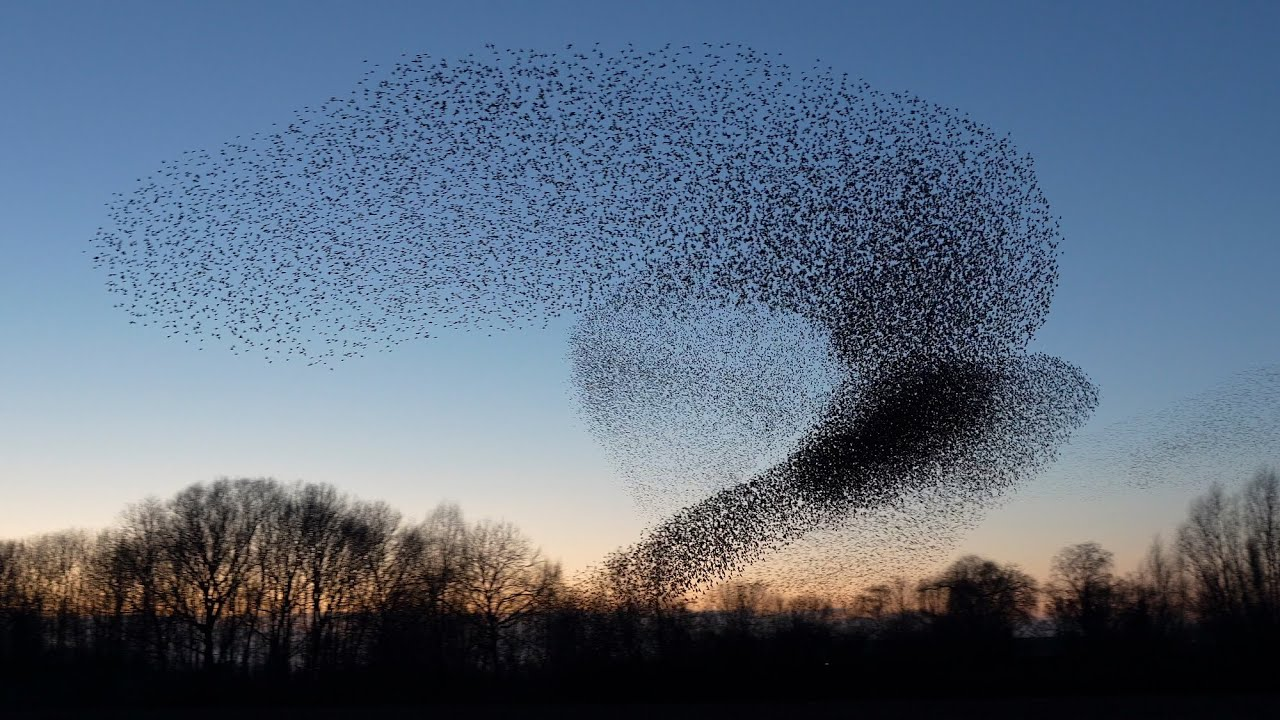
\includegraphics[width=0.35\textwidth]{illustrations/starling_flocking.jpg}
  \caption{Ein Starenschwarm als klassisches Beispiel für Schwarmdynamik~\cite{starenschwarm}.}
  \label{fig:starling_flocking}
\end{wrapfigure}

Die Eigenschaft eines Kollektivs, differenziertes Verhalten aus simplen, häufig trivialen Entscheidungen einzelner Individuen zu entwickeln, birgt eine Universalität, die bis heute noch nicht ganz verstanden ist. Die wissenschaftliche und gesellschaftliche Relevanz kollektiven Verhaltens ist weitreichend.\\

Bislang gibt es in der Wissenschaft kein universelles Modell zur Beschreibung von Schwarmverhalten. Frühere metrische Modelle, insbesondere das von \textit{Vicsek et al.} \cite{vicsek1995}, werden zunehmend von topologischen Ansätzen abgelöst, um reale Szenarien besser zu beschreiben. So hat sich gezeigt, dass topologische Modelle bei der Beschreibung von Vogelschwärmen zuverlässigere Vorhersagen ermöglichen als metrische Modelle \cite{InteractionRulingAnimal2007}. Das von \textit{Vicsek et al.} vorgestellte Modell ist seit 1995 der Grundstein der mathematischen Beschreibung von Schwärmen. Viele fortgeschrittene Modelle, wie etwa das Boids-Modell \cite{reynolds1987}, sind Weiterentwicklungen des Vicsek-Modells und es ist nicht ungewöhnlich, dass neue Modelle und Konzepte das Vicsek-Modell erwähnen oder verwenden.
\textit{Tamàs Vicsek} war auch die treibende Kraft hinter der sehr umfangreichen Review ``\textit{Collective Motion}'' \cite{CollectiveMotionVicsek2012} und beschäftigte sich fortwährend mit der Tragweite dieses Themas.\\

Trotz der frühen Entwicklung dieses Forschungsbereichs bieten die aktuell zur Verfügung stehenden Modelle zur Bildung von Schwärmen nur eingeschränkte Möglichkeiten zur Erklärung der beobachteten Phänomene, insbesondere, wenn es um die Ausbildung von Schwärmen in künstlichen Systemen geht. Diese Arbeit zielt darauf ab, diese Herausforderung anzugehen, indem eine Schnittstelle zwischen traditionellen physikalischen Modellen und modernen Methoden des Maschinellen Lernens geschaffen wird. Dabei liegt der Fokus auf zeitaufgelöste topologische Strukturen.\\

Ausgangspunkt bildet das eben genannte Vicsek-Modell. Das Modell wird ergänzt durch die Einführung eines neuartigen Metrisch-Topologischen Modells mit stochastischen Elementen, das im Zuge dieser Arbeit speziell dafür entwickelt wurde, um die Integration von Maschinellem Lernen zu erleichtern. Für die hochdynamischen Vielteilchen-Umgebungen werden Algorithmen des Multi-Agent Reinforcement Learning (MARL) verwendet, die auf dem Training neuronaler Netze basieren.\\

Mit dem Einsatz von Reinforcement Learning wird eine fundamentale Neuausrichtung in der Modellierung der Schwarmdynamik eingeführt. Hier stehen nicht länger die lokal implementierten Regeln im Mittelpunkt, sondern die übergeordneten Ziele des Schwarms. Die Agenten lernen eigenständig die für das Erreichen dieser Ziele erforderlichen Verhaltensmuster. Als Ziel können Ordnungsparameter definiert werden, welche eine mathematische Beschreibung eines Systemzustandes darstellen. Diese Ordnungsparameter sind bedeutend aussagekräftiger und einfacher zu entwickeln als eine lokale Entscheidungsregel.\\

Diese Arbeit legt zunächst das theoretische Fundament, um die angewandten Konzepte ausreichend zu verstehen und nachvollziehen zu können. Anschließend wird systematisch skizziert, wie die Implementation einer Schwarmsimulation durchgeführt wurde, da diese im Kern dieser Arbeit steht. Es wird das Vicsek-Modell und seine topologische Modifikation nachgebildet und untersucht. Dieses Modell wird durch die bereits erwähnten metrisch-topologischen Eigenschaften erweitert und damit deutlich verbessert. Zum Schluss wird die MARL-Implementation erläutert und diskutiert.

\newpage

\section{Theoretische Grundlagen}
Die Schwarmdynamik befasst sich mit zeitabhängigen topologischen Strukturen von Vielteilchensystemen. Sie kann also im Kontext der statistischen Physik betrachtet werden. Ähnlich wie in konventionellen Systemen der kondensierten Materie, in denen Phasenübergänge, kritische Exponenten und universelle Verhaltensmuster eine Rolle spielen, zeigt die Schwarmdynamik bemerkenswerte Analogien zu diesen Phänomenen. Indem Schwärme als stochastische, nichtlineare Systeme vieler interagierender Einheiten betrachtet werden, wird es möglich, Methoden der statistischen Physik anzuwenden, um emergente kollektive Verhaltensweisen zu analysieren. Diese Sichtweise ermöglicht das Einführen von Phasen, die Untersuchungen des Verhaltens an kritischen Punkten und die Definition von kritischen Exponenten sowie die Charakterisierung des Verhaltens in der Nähe von Phasenübergängen. In dieser Arbeit werden diese Aspekte jedoch nur phänomenologisch untersucht.

Eine konkrete Manifestation dieser Konzepte bietet das Vicsek-Modell, das im nächsten Abschnitt detailliert behandeln wird. 

\subsection{Vicsek-Modell}
Eines der einfachsten und grundlegendsten Modelle für die Simulation von Schwärmen ist das Vicsek-Modell \cite{vicsek1995}. In diesem zweidimensionalen Modell können die Teilchen nur in einem bestimmten Wechselwirkungsradius miteinander interagieren und haben eine konstante Geschwindigkeit $v_0$. Der Betrag der Geschwindigkeit wird durch die Wechselwirkungen nicht beeinflusst.
Den einzigen Aktionsraum, den die Teilchen zur Verfügung haben, ist die Änderung ihres eigenen Winkels
$\theta_i$. Diese Änderung entspricht dem Mittelwert der Richtung aller Teilchen, die sich in dem Wechselwirkungsradius $r$ befinden. Charakterisiert wird das System durch einige weitere Parameter, die in Tabelle \ref{table:vicsek_parameters} aufgelistet sind.

\begin{table}[h]
    \centering
    \caption{Parameter des Vicsek-Modells.}
    \label{table:vicsek_parameters}
    \begin{tabular}{|c|l|}
        \hline
        \textbf{Parameter} & \textbf{Beschreibung} \\
        \hline
        \(v_0\) & Konstante Geschwindigkeit aller Teilchen \\
        \(\theta_i\) & Winkel des \(i\)-ten Teilchens \\
        \(r\) & Wechselwirkungsradius für die Nachbarauswahl \\
        \(L\) & Länge des quadratischen Simulationsbereichs \\
        \(N\) & Anzahl der Teilchen \\
        \(\rho = \frac{N}{L^2}\) & Teilchendichte \\
        \(\eta\) & Rauschintensität (Noise) \\
        \(v_a\) & Ordnungsparameter: quantifiziert den Grad der Ausrichtung \\
        $t$ & Simulationszeit \\
        \hline
    \end{tabular}
\end{table} 

Der Parameter $\eta$ repräsentiert hierbei ein stochastisches Rauschen, das als kleine Störung $\Delta \theta_i$ dem Winkel $\theta_i(t+1)$ \eqref{eq:next_angle} eines Teilchens hinzugefügt wird. Die Intensität dieses Rauschens beeinflusst den makroskopischen Zustand des Schwarms und kann durch Variation bei sonst gleichbleibenden Parametern zu unterschiedlichen Phasen des Systems führen. In weiterführenden topologischen Modellen kann unter bestimmten Bedingungen zudem die \textit{Koexistenz} mehrerer Phasen gezeigt werden.

In der ursprünglichen Arbeit wird ein quadratischer Simulationsbereich mit Länge $L$ und periodischen Randbedingungen gewählt. Des Weiteren wurden alle Simulationen bei konstanter Geschwindigkeit $v_0 = \SI{0.03}{\meter\per\second}$ durchgeführt, was in der Gesamtheit dieser Arbeit übernommen wird.

\divider

\textbf{Charakteristische Größen}

Das Modell wird durch den Wechselwirkungsradius $r [\si{\meter}]$ und der konstanten Geschwindigkeit $v_0 [\si{\meter\per\second}]$ charakterisiert und darüber entdimensionalisiert. Ein Simulationsschritt entspricht dann der charakteristischen Zeit $\tau = \frac{r}{v_0}$. Daraus ergeben sich die dimensionslosen Größen $\Tilde{t} = \frac{t}{\tau}$ für die Zeit, $\Tilde{r}_k = \frac{r_k}{r}$ für die kartesischen Ortskoordinaten und $\Tilde{v}_k = \frac{v_k}{v_0}$ für die Geschwindigkeiten (mit $k \in {x, y}$). Hierdurch sind die Vektoren $\Tilde{\vec{x}}_i$ und $\Tilde{\vec{v}}_i$ (bezogen auf das $i$-te Teilchen) ebenfalls einheitenlos. Für einen einzelnen Simulationsschritt gilt dann $\Delta \Tilde{t} = 1$.


\subsection*{Mathematische Beschreibung des Vicsek-Modells}
In der Schwarmdynamik, insbesondere im Kontext des Vicsek-Modells, ist die Frage der Energieerhaltung oft weniger zentral als in der klassischen Mechanik. Die Modelle sind in der Regel eher phänomenologisch und zielen darauf ab, bestimmte Aspekte kollektiven Verhaltens zu reproduzieren, anstatt von fundamentalen physikalischen Prinzipien auszugehen. Statt eines Verlet-Algorithmus oder anderen symplektischen Integratoren, die den Hamiltonschen Fluss erhalten, wird hier ein einfaches Euler-Verfahren für die Aktualisierung der Teilchenpositionen verwendet:

\begin{equation}
    \Tilde{\vec{x}}_i(\Tilde{t}+1)=\Tilde{\vec{x}}_i(\Tilde{t})+\Tilde{\vec{v}}_i(\Tilde{t}) \Delta \Tilde{t}
    \label{eq:euler}
\end{equation}

Hierbei wird die Geschwindigkeit $\vec{v}_i(\Tilde{t} + 1)$ derart konstruiert, dass ihr Betrag die charakteristische Geschwindigkeit erhält und die Winkeländerung $\theta(\Tilde{t}+1)$ erfährt. Der aktualisierte Winkel eines Teilchens setzt sich dann aus dem Mittel der Winkel seiner Nachbarn und aus einem stochastischen Element zusammen:

\begin{equation}
    \theta(\Tilde{t}+1)=\langle\theta(\Tilde{t})\rangle_r+\Delta \theta \quad .
    \label{eq:next_angle}
\end{equation}

Der Ausdruck $\langle\theta(\Tilde{t})\rangle_r$ entspricht einer Mittelung über die Winkel aller Teilchen im Wechselwirkungsradius $r$; einschließlich des Teilchens selbst. Der durchschnittliche Winkel wird über

\begin{equation}
    \langle\theta(\Tilde{t})\rangle_r = \arctan \left[ \frac{\langle\sin (\theta(\Tilde{t}))\rangle_r}{\langle\cos (\theta(\Tilde{t}))\rangle_r} \right]
    \label{eq:vicsek_rule}
\end{equation}

berechnet. Die Zufallszahl $\Delta \theta$ wird uniform aus dem Intervall $[-\eta / 2, \eta / 2]$ generiert. Um die Gleichverteilung dieser Störung nicht zu verletzen, sollte $\eta$ in $[0, 2 \pi)$ liegen, da es ansonsten Winkelbereiche gibt, die stärker gewichtet werden.\\

Als zentraler Kennwert wird der \textbf{Ordnungsparameter} $v_a$ eingeführt:

\begin{equation}
    v_a=\frac{1}{N v_0}\left|\sum_{i=1}^N \vec{v}_i\right| \quad .
    \label{eq:ordnungsparameter_vicsek}
\end{equation}

Dieser normierte, skalare Ausdruck quantifiziert den Grad der Ausrichtung oder Kohäsion innerhalb des Schwarms.

Ein System, in dem alle Teilchen in dieselbe Richtung zeigen, hat $v_a = 1$, während ein vollständig \textit{ungeordnetes} System $v_a \approx 0$ aufweist; es gilt also $v_a \in [0,1]$.

Dieser Parameter enthält keine Information über die Dichte, Kohäsion oder topologische Cluster-Bildung eines Schwarms. Es zeigt sich jedoch, dass sowohl die einfache Mittelungs-Regel des Vicsek-Modells als auch der Ordnungsparameter $v_a$ ausreichen, um Schwärme zu bilden und quantitativ zu beschreiben. Ferner kann analytisch gezeigt werden, dass die Vicsek-Regel ebendiesen Ordnungsparameter $v_a$ minimiert (siehe Abschnitt \ref{sec:Vicsek_Modell_Analytisch}).

\divider

Das Vicsek-Modell hat drei freie Parameter: Die Teilchenzahl $N$, die Rauschintensität $\eta$ und die Länge des Dimensionsbereiches $L$. Bewertet wird das Modell nach dem Ordnungsparameter. Daraus ergeben sich viele mögliche Kombinationen, die untersucht werden können. In der ursprünglichen Arbeit \cite{vicsek1995} und in vielen darauf aufbauenden Arbeiten \cite{PhaseTransitions2013}, \cite{Aldana_2007} werden jedoch nur die Rauschintensität $\eta$ und die Dichte $\rho$ gegen den Ordnungsparameter aufgetragen und untersucht.

Der Fokus auf die Dichte \( \rho \) ist insofern sinnvoll, als sie direkten Aufschluss über die mittlere Anzahl der Wechselwirkungspartner gibt. Formell gilt
 
\begin{equation}
    n_r = \rho \pi r^2 = N \frac{\pi r^2}{L^2} \quad .
    \label{eq:Wechselwirkungsradius}
\end{equation}


Hierbei ist \( n_r \) dimensionslos und gibt an, wie viele benachbarte Teilchen sich im Mittel im Wechselwirkungsradius \( r \) des betrachteten Teilchens aufhalten. Diese dimensionslose Größe erlaubt eine effizientere numerische Analyse, fördert die Vergleichbarkeit mit anderen Arbeiten und ist physikalisch relevanter als die einzelne Variation von \( N \) und \( L \).

Da das System entdimensionalisiert ist, gilt sogar direkt $\Tilde{n}_r = \pi \rho$. Aus der Dichte ist diese Größe also um einen Faktor von $\pi$ direkt ablesbar. Dies erweitert die Interpretierbarkeit vieler Plots.\\

Es sei allerdings erwähnt, dass dies nur einer Näherung für equilibrierte Systeme entspricht. Dort können die Teilchen als gleichverteilt und die Dichte als annähernd homogen betrachtet werden, sodass die einzelnen Beiträge einer ortsbasierten Dichte $\rho (r)$ durch ihre statistische Unabhängigkeit faktorisiert werden können. Daher gilt dieser Ausdruck nur in 0. Ordnung. Für eine rigorose Auseinandersetzung mit der Wechselwirkungspartner-Anzahl werden fortgeschrittenere Ansätze benötigt. An dieser Stelle wird ein Dichte-basierter Ordnungsparameter motiviert, der in Abschnitt \ref{sec:Dichte_Parameter} eingeführt wird.\\

\textbf{Visuelle Repräsentation des Vicsek-Modells}

Angelehnt an die originale Arbeit werden in Abbildung \ref{fig:vicsek_snapshots} einige Schnappschüsse einer Simulation gezeigt. Zusammengehörende Parametersätze sind farblich hervorgehoben.

\begin{figure}[h!]
    \centering
    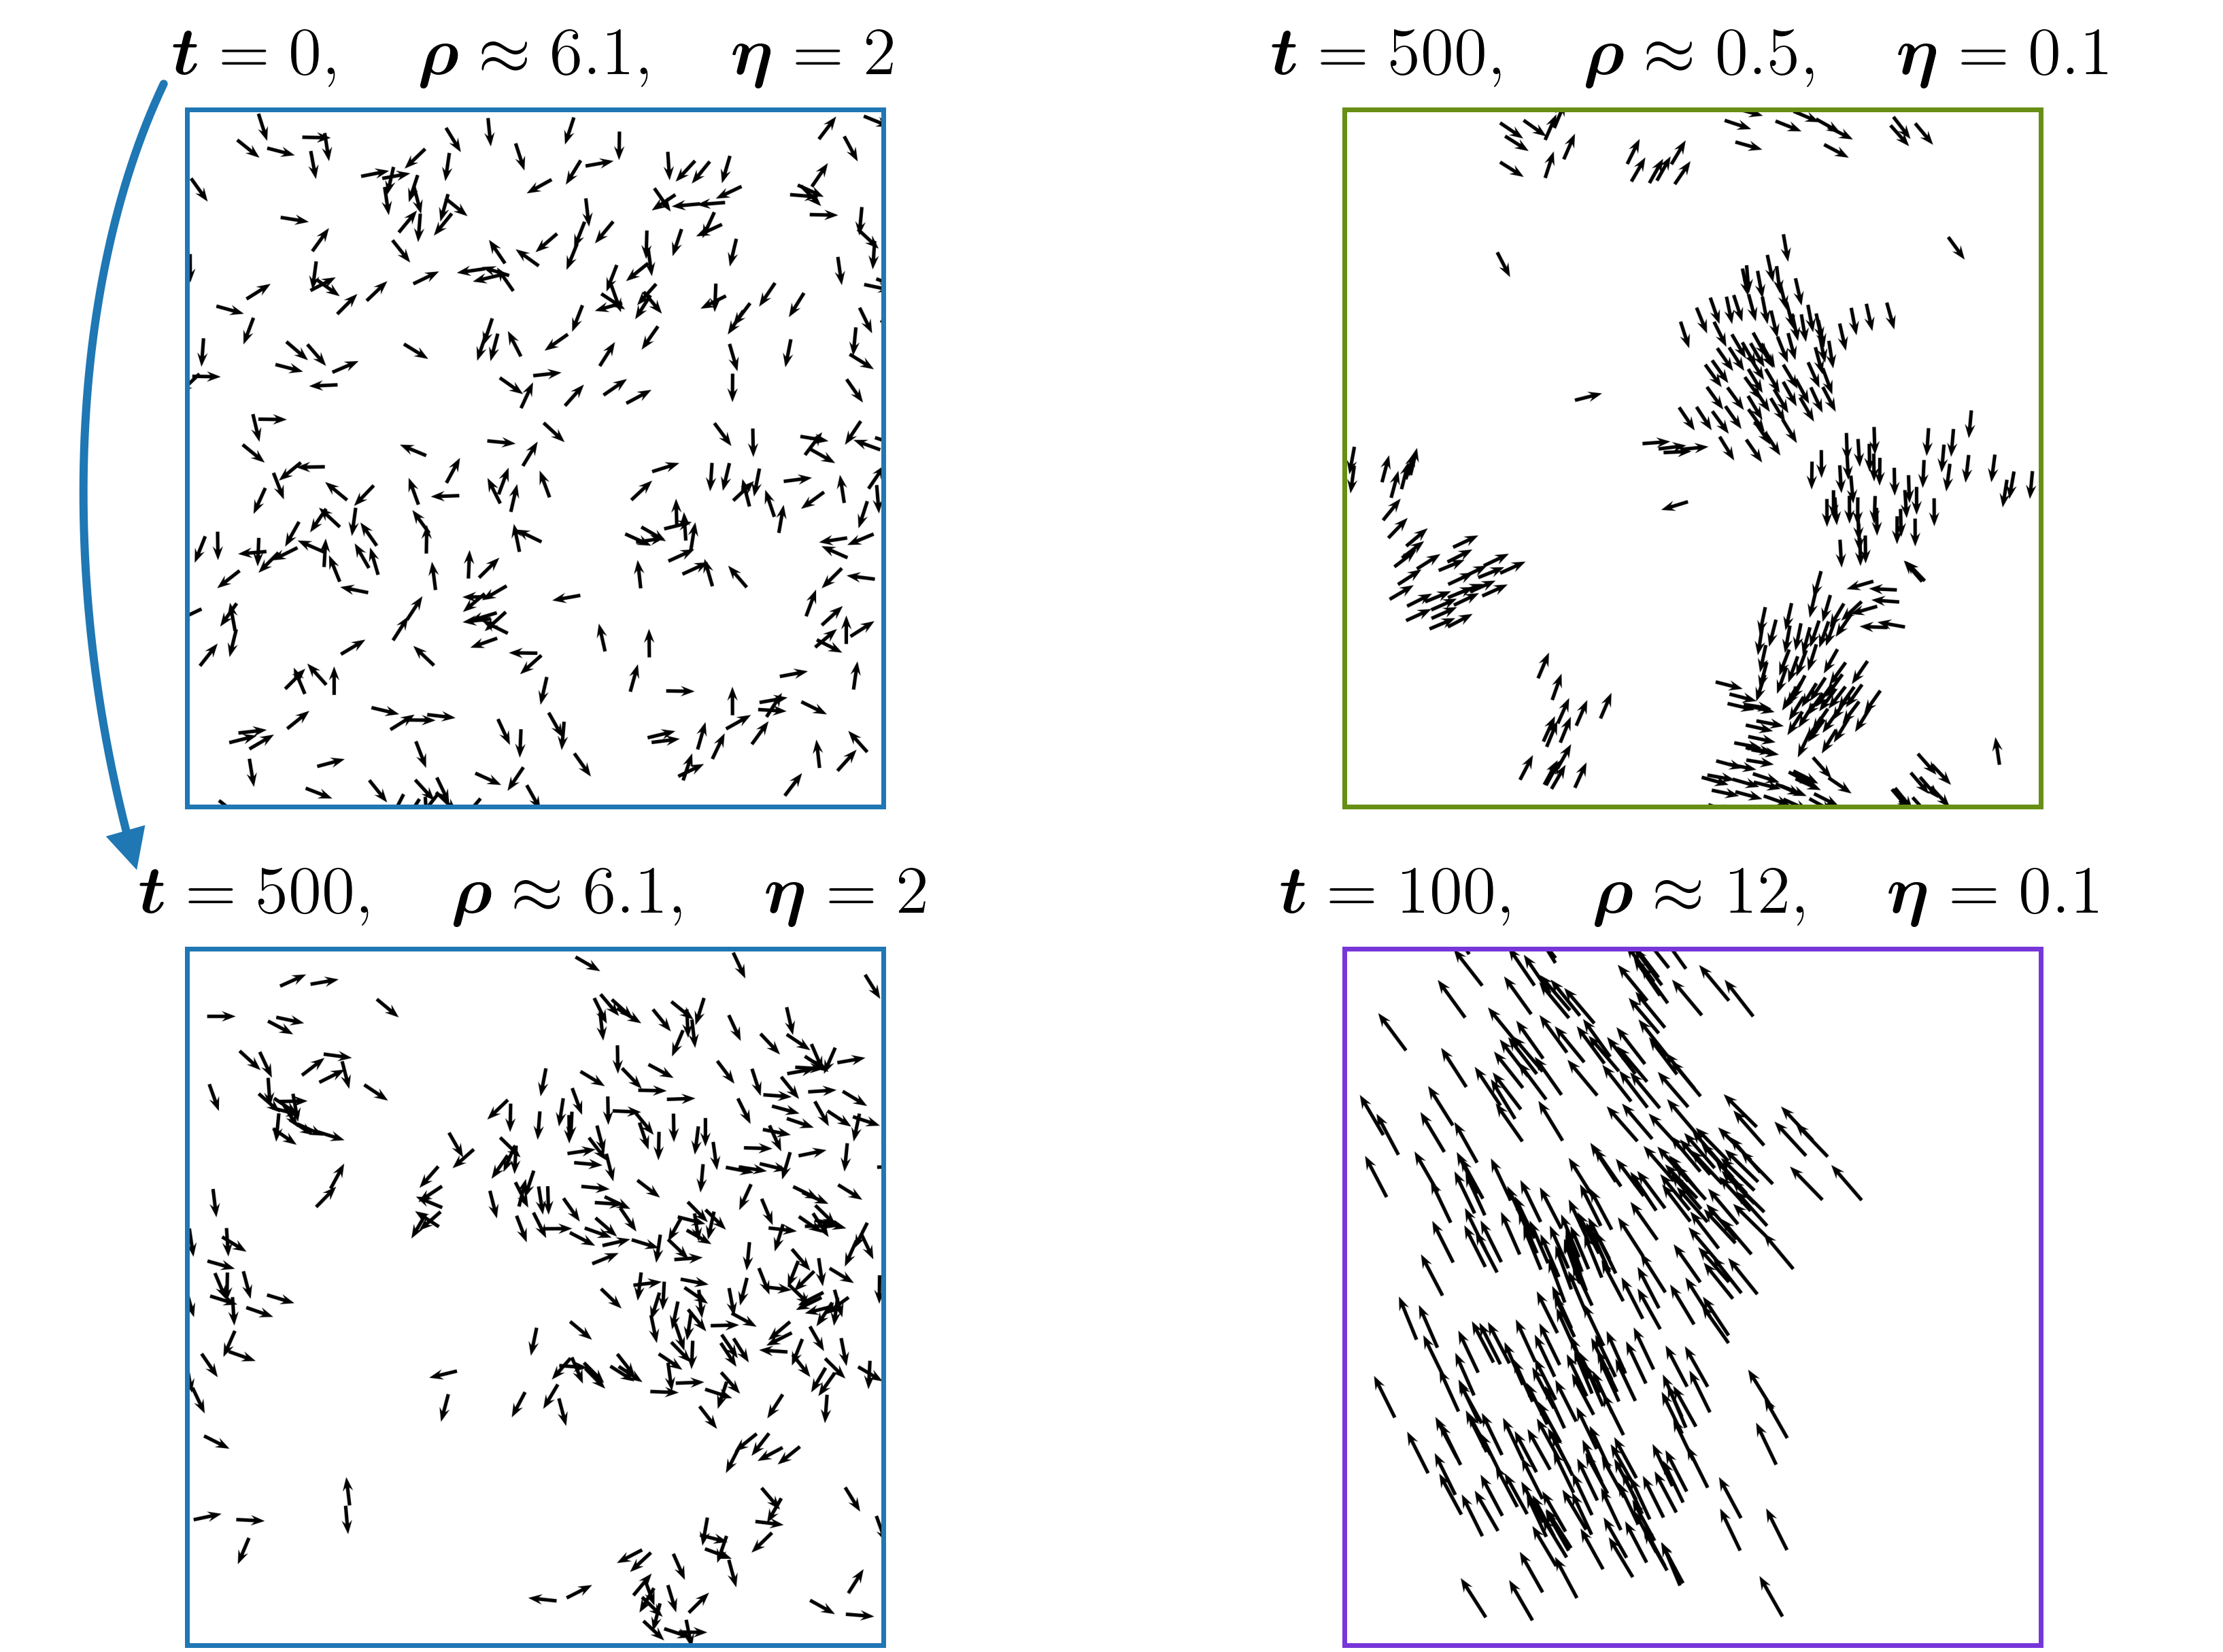
\includegraphics[width=.9\textwidth]{illustrations/Vicsek_Schnappschuss_clipped.png}
    \caption{Vier Szenarien des Vicsek-Modells mit \(N=300\) Teilchen. Die beiden \textcolor{matplot_C0}{blauen Plots} zeigen zwei Zeitpunkte \(t=0\) und \(t=500\) bei \(L=7\). Der \textcolor{DTUGreen}{grüne Plot} stellt \(t=500\) bei \(L=25\) und niedriger Dichte \(\rho \approx 0.5\) dar. Der Plot im \textcolor{TUCLight}{lilanen Rahmen} zeigt \(t=100\) bei \(L=5\) und hoher Dichte \(\rho \approx 12\). Die Schnappschüsse stammen aus der eigenen Simulation und wurden mit Matplotlib \cite{Matplotlib2007} visualisiert.}
    \label{fig:vicsek_snapshots}
\end{figure}

\newpage

\subsection{Metrische und Topologische Modelle}
Die meisten grundlegenden Modelle zur Schwarmdynamik können in metrische und topologische Modelle unterteilt werden. Metrische Modelle bestimmen die Nachbarn eines Teilchens auf Basis eines Abstandes, während topologische Modelle eine \textit{feste Anzahl} von \textit{nächsten} Nachbarn wählen; unabhängig von der Distanz.

In Abbildung \ref{fig:Metrisch_vs_Topologisch} sind diese beiden Auswahlregeln gegenübergestellt.

\begin{figure}[h!]
    \centering
    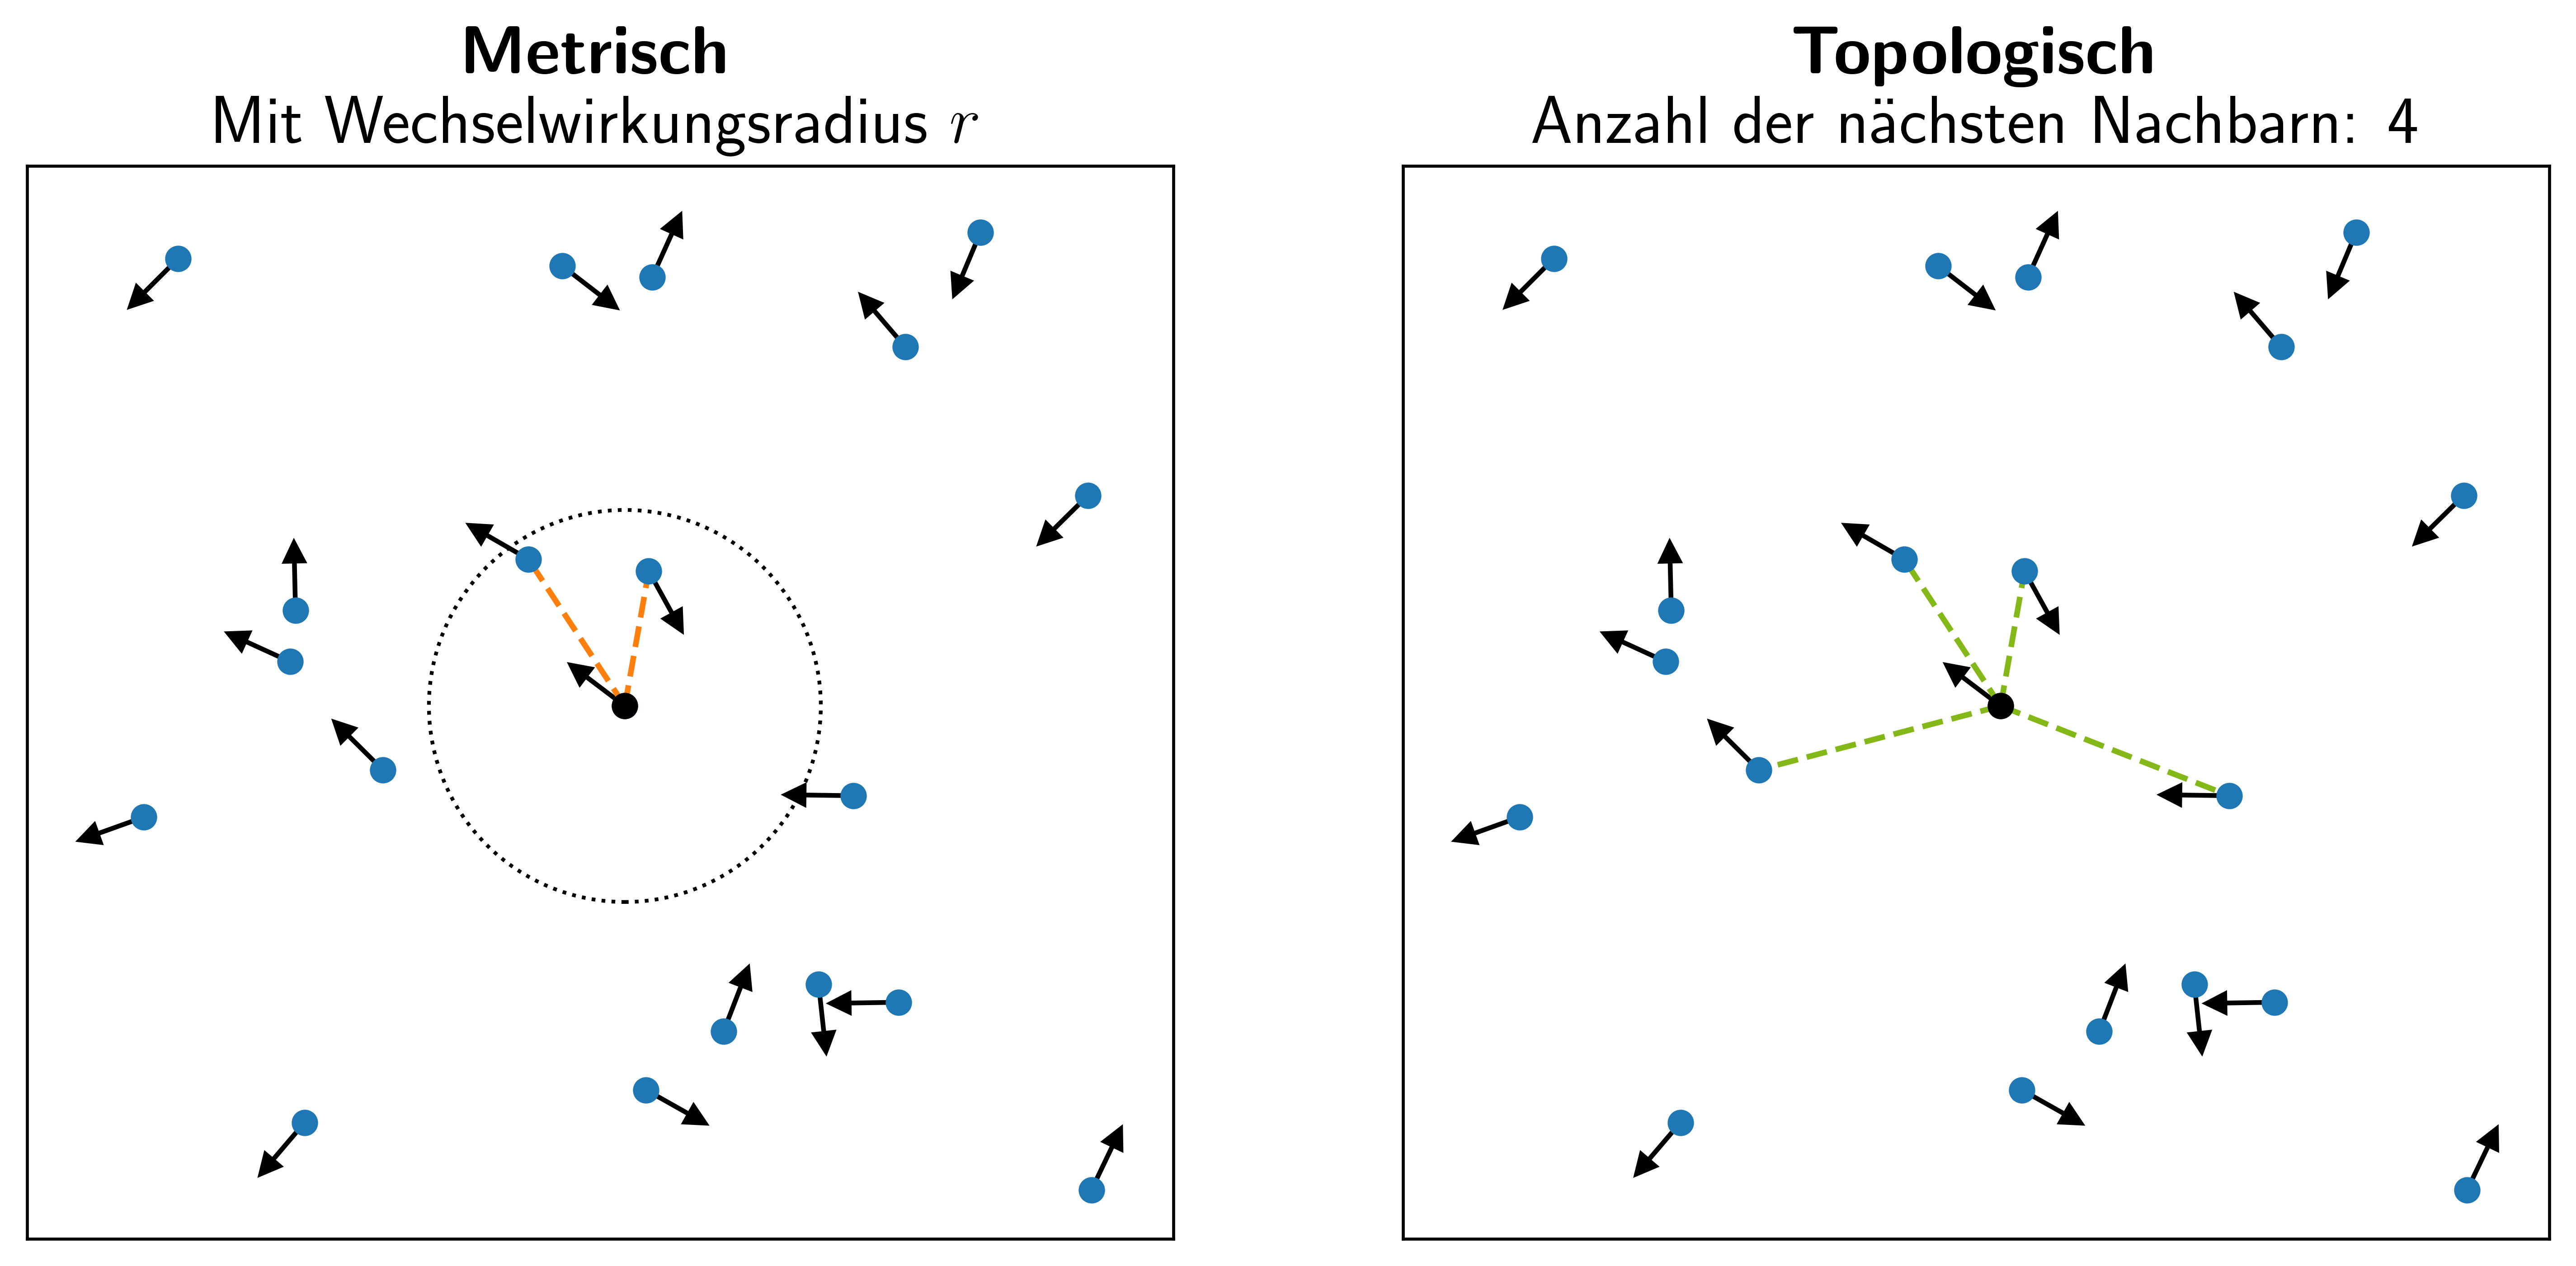
\includegraphics[width=.9\textwidth]{illustrations/metric_vs_topologic.png}
    \caption{Vergleich zwischen metrischer und topologischer Nachbarschaftsauswahl in einem Schwarm von 20 Teilchen. Beispielhaftes Ermitteln der Nachbarn für ein Teilchen (zentriert). Die gestrichelten Verbindungslinien stellen die ermittelten Nachbarn dar. \newline\textbf{Links:} In der metrischen Auswahl werden Nachbarn in einem festen Wechselwirkungsradius $r$ (gestrichelter Kreis) bestimmt.
    \newline \textbf{Rechts:} In der topologischen Auswahl werden \textit{immer} $k$ Nachbarn gefunden (falls $N > k$), unabhängig von ihrer räumlichen Entfernung.
    \newline Hier beispielhaft: $k = 4$.
    \newline Die Teilchenverteilung und -Ausrichtung sind in beiden Plots identisch.}
    \label{fig:Metrisch_vs_Topologisch}
\end{figure}

Mit dem Vicsek-Modell wurde bereits ein metrisches Modell vorgestellt. Weitere metrische Modelle sind bspw. das Boids-Modell \cite{reynolds1987} oder das Cucker-Smale-Modell \cite{cuckerSmale2007}. Beide Modelle können jedoch als Weiterentwicklung des Vicsek-Modells verstanden werden.\\

Für diese Arbeit sind vor allem topologischen Modelle interessant, da diese eine feste Anzahl an Nachbarn vorgeben. Dies vereinfacht eine Implementierung der meisten Algorithmen des Maschinellen Lernens, da neuronale Netze eine feste Länge des Eingabevektors voraussetzen (Ausnahme sind die fortgeschrittenen Recurrent Neural Networks (RNNs) \cite{ElmanRNN} und Transformers \cite{Transformers2017}). In diesem Kontext ist die alleinige Modifikation der Nachbarschaftsregel von metrisch zu topologisch, bei sonst unveränderten Simulationsparametern, besonders relevant. Der Wechselwirkungsradius $r$ verliert dann seine Bedeutung, kann aber als Vorbereitung auf ein weiterführendes metrisch-topologisches Modell behalten werden. Dies erleichtert einen direkten Vergleich.

In einer vorangegangenen Studie wurde die topologische Modifikation des Vicsek-Modells bereits untersucht \cite{PhaseTransitions2013}. Dort wurden sowohl Gemeinsamkeiten als auch Unterschiede der beiden Modelle beobachtet.

Auf die Details und einen direkten Vergleich der Modelle wird in der Nachbildung der Modelle in Abschnitt~\ref{sec:Nachbildung} eingegangen.

\subsection{Grundlagen Maschinelles Lernen}
In der Einleitung wird die Verwendung Maschinellen Lernens bereits motiviert. Die Herausforderung besteht nun darin, einen Algorithmus und ein Framework zu wählen, die für das Problem geeignet sind. In Anbetracht der Vielfalt der Ansätze, die alle ihre eigenen Vor- und Nachteile mitbringen, und angesichts der rapiden Entwicklung in diesem Forschungsbereich, wird zunächst eine Klassifizierung des Problems vorgenommen und die zurzeit verfügbaren Methoden werden kurz skizziert und bewertet.\\

\textbf{Klassifizierung des Problems}

In konventionellen Schwarm-Simulationen wird über jedes Teilchen iteriert und anhand der Beobachtung des Teilchens über eine feste Regel eine Aktion generiert, die bspw. in den einfachen Modellen zu einer Winkeländerung des Teilchens führen. Da die Qualität der Schwarm-Bildung über einen einzigen, skalaren Parameter bewertet wird, liegt kein Klassifizierungs- oder Regressions-Problem im klassischen Sinne vor.

Vielmehr soll ein Teilchen ein Verhalten bzw. eine \textit{Strategie} entwickeln, die diesen einfachen Parameter maximiert; und im entsprechenden Sinne Aktionen bestraft, die zur Verringerung dieses Parameters führen.\\

Diese Begriffe und Konzepte sind eng verwandt mit dem \textbf{Reinforcement Learning}; ein Bereich des Maschinellen Lernens, der weder dem überwachten noch unüberwachten Lernen zuzuordnen ist. \\

\textbf{Reinforcement Learning}

Das Reinforcement Learning (RL) stellt eine Reihe von Methoden dar, bei der ein Agent selbstständig lernt, in einer Umgebung unter verschiedenen Beobachtungen eine vorgegebene Belohnung zu maximieren. In diskreten und einfacheren RL-Algorithmen wird oft mit einer Tabellenrepräsentation des Zustands- und Aktionsraums gearbeitet, welche auf Grundlage neuer Beobachtungen und Belohnungen aktualisiert werden. Diese Aktualisierung stellt dann das Training dar. Fortgeschrittene Methoden benötigen komplexere Strukturen als Tabellen; insbesondere für das Training. Das in Abbildung \ref{fig:Basic_RL_concept} skizzierte Konzept bleibt allen Algorithmen jedoch gleich.

\begin{figure}[h!]
    \centering
    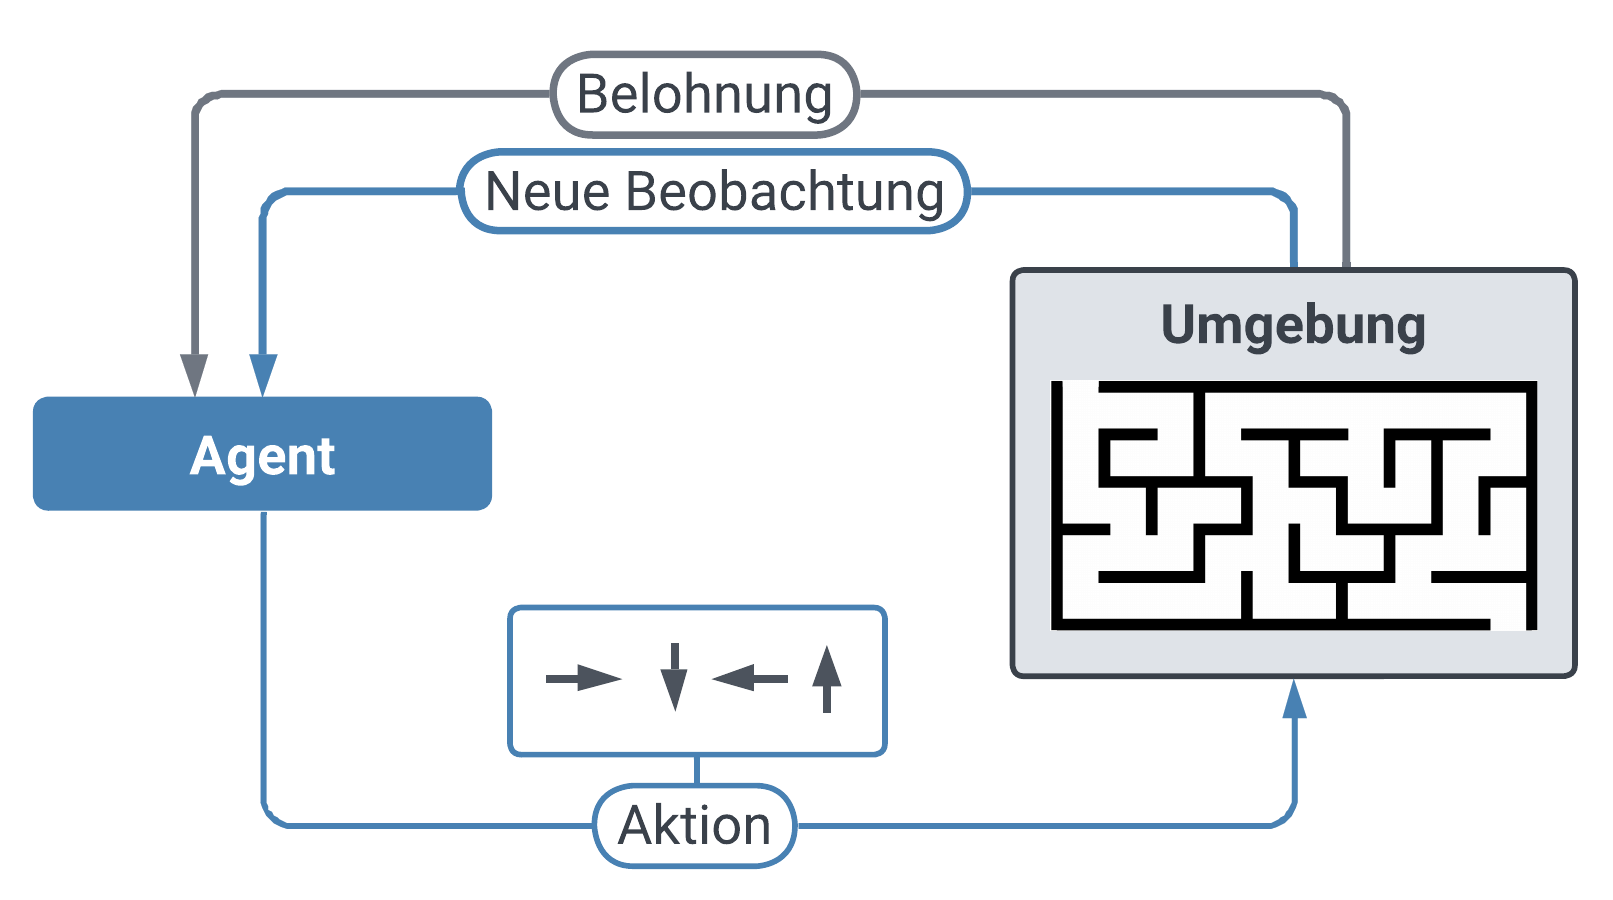
\includegraphics[width=.7\textwidth]{illustrations/Basic_RL_concept.png}
    \caption{Grundlegendes Konzept des Reinforcement Learning: Ein Agent trifft in einer gegebenen Umgebung eine Aktion, woraufhin er eine Belohnung sowie eine neue Beobachtung der Umgebung erhält. Diese Interaktion ermöglicht es dem Agenten, seine Entscheidungsstrategie iterativ zu verbessern, um kumulative Belohnungen zu maximieren.}
    \label{fig:Basic_RL_concept}
\end{figure}

Im Reinforcement Learning werden einige Begriffe eingeführt, die in der Literatur einheitlich verwendet werden. Dies vereinfacht die Übersetzung eines vorliegenden Problems in eine Form, die alle Algorithmen verstehen. Fortgeschrittene Methoden führen weitere Konzepte und Begriffe ein, die aber klar abgegrenzt werden können. Eine Übersicht der grundlegenden Begriffe ist in Tabelle \ref{tab:RL_basic_terms} zu finden.

Literatur zu diesem Teil: Bonaccorso, \textit{Mastering Machine Learning Algorithms} \cite{bonaccorso2018mastering}.

\begin{table}[h!]
    \centering
    \caption{Grundbegriffe des Reinforcement Learnings.}
    \label{tab:RL_basic_terms}
    \begin{tabular}{|p{2.4cm}|p{11cm}|} % Hier p{width} für die Breite der Spalten setzen.
        \hline
        \textcolor{DTUGreen}{\textbf{Begriff}} & \textcolor{DTUGreen}{\textbf{Beschreibung}} \\
        \hline
        \hline
        \textbf{Agent} & Autonomer Entscheidungsträger, der auf Grundlage einer Beobachtung Aktionen in einer Umgebung ausführt, um eine Belohnung zu erhalten. \\
        \hline
        \textbf{Umgebung} \newline \textit{(environment)} & Der Kontext oder Raum, in dem der Agent operiert und in dem Zustände, Aktionen und Belohnungen definiert sind. \\
        \hline
        \textbf{Zustand} \newline \textit{(state) \newline \(s \in \mathcal{S}\)} & Spezifische Konfiguration (Beobachtung) der Umgebung, die alle relevanten Informationen enthält, die der Agent zum Treffen einer Entscheidung benötigt. \\
        \hline
        \textbf{Aktion} \newline  \textit{(action) \newline \(a \in \mathcal{A}(s)\)} & Eine Operation oder ein Vorgang, den der Agent in einem bestimmten Zustand (\(s\)) ausführt, um seinen Zustand in der Umgebung zu ändern. \\
        \hline
        \textbf{Belohnung} \newline \textit{(reward) \newline \(r: \mathcal{S} \times \mathcal{A} \rightarrow \mathbb{R}\)} & Ein numerischer Wert, der dem Agenten als Feedback für seine Aktion in einem bestimmten Zustand zurückgegeben wird. Ziel ist es, die kumulierte Belohnung zu maximieren. \\
        \hline
        \textbf{Strategie} \newline \textit{(policy) \newline \( \pi: \mathcal{S} \rightarrow \mathcal{A} \)} & Ein Regelwerk oder Algorithmus, den der Agent verwendet, um in einem bestimmten Zustand eine Aktion auszuwählen. \\
        \hline
        \textbf{Value-Funktion $V$} & Eine Funktion, die den erwarteten kumulativen zukünftigen Belohnungswert für einen gegebenen Zustand (\(s\)) schätzt. Sie dient als Grundlage für die Entscheidungsfindung des Agenten und wird in vielen RL-Methoden aktualisiert. \newline Typische Darstellung: $V^\pi(s) = \mathbb{E}[R_t | s_t = s, \pi]$ \\
        \hline
        \textbf{Episode} & Sequenz von (Zeit-)Schritten, die der Agent durchläuft, um Aktionen auszuführen und Belohnungen zu erhalten. Kann endlos sein; manche Algorithmen benötigen jedoch ein explizites Ende (bspw. ein Spiel, das gewonnen oder verloren wird). In dieser Arbeit kann das Erreichen eines Gleichgewichtszustands als implizites Ende fungieren. \\
        \hline
    \end{tabular}
\end{table}

\subsection{MARL und PPO}

Das Multi-Agent Reinforcement Learning (MARL) ist ein sehr junges und sich schnell entwickelndes Forschungsfeld, das viele bisher ungesehene algorithmische Herausforderungen und Anwendungsfälle bietet \cite{MARLReview2021, CityFlow2019}. Vorreiter in der Entwicklung und Untersuchung neuer MARL Algorithmen ist OpenAI. Im vorangegangenen Abschnitt wurden die Grundlagen des Reinforcement Learnings erläutert. Der folgende Abschnitt vertieft das Verständnis dieser Konzepte durch die Einführung von MARL und Proximal Policy Optimization (PPO). Während MARL eine Erweiterung des Reinforcement Learnings auf mehrere Agenten darstellt, ist PPO ein konkreter Algorithmus zur Optimierung einer Strategie. Beide Konzepte werden in dieser Arbeit verwendet.\\

In diesem Theorieteil werden bereits methodologische Elemente integriert, da sie in diesem Kontext am sinnvollsten erscheinen. Somit geht es im Folgenden nicht nur um allgemeine Konzepte, sondern auch um deren spezifische Anwendung im Kontext der in dieser Arbeit entwickelten Simulation.

\subsection*{Multi-Agent (MA) Systeme}
Im klassischen Reinforcement Learning wird nur ein einzelner Agent betrachtet, der eine Strategie in einer Umgebung lernt und optimiert. Bei Vielteilchensystemen, wie etwa der vorliegenden Schwarmsimulation, ändert sich die Herangehensweise grundlegend. Es ergeben sich vollkommen neue Fragestellungen und Herausforderungen. Eine Umgebung und ein Programm, die für einen einzelnen Agenten geschrieben wurden, können nicht ohne Weiteres auf ein Multi-Agent System erweitert werden. In diesem Theorieteil werden nur die konzeptionellen Fragen und einige grundlegende Aspekte beleuchtet. Die technischen Herausforderungen und die konkrete Methodologie werden im entsprechenden Abschnitt \ref{sec:Neuronale_Schwarmdynamik} erläutert.\\

\textbf{MARL als Erweiterung des Reinforcement Learnings}

Bei der Umstellung auf mehrere Agenten ergeben sich einige Veränderungen im algorithmischen Kern.

\begin{itemize}
    \item \textbf{Datengranularität}: Während im klassischen RL Zustände, Aktionen und Belohnungen einzelner Agenten betrachtet werden, müssen diese Elemente im MARL für eine ganze Gruppe von Agenten gemeinsam erfasst werden. Hierbei werden die Daten in der Regel \textit{gebatched}, d.h., sie werden für mehrere Agenten gleichzeitig gesammelt und verarbeitet. Dadurch muss die \textit{Umgebung} fundamental neu implementiert werden und das Handling von Zustands- und Aktions-Vektoren, insbesondere angesichts der Verwendung neuronaler Netze, wird wesentlich empfindlicher.
    \item Handling der \textbf{Value-Funktion}: Diese bewertet nun den Gesamtnutzen mehrerer Agenten und muss oft unter Berücksichtigung der Aktionen und Zustände aller beteiligten Agenten berechnet werden.
    \item Kompliziertere \textbf{Strategieentwicklung}: In MARL wird nicht nur die Komplexität der möglichen Strategien erhöht, sondern auch die Notwendigkeit, diese Strategien effektiv an mehrere Agenten zu verteilen. Das kann bedeuten, dass eine geteilte Strategie an alle Agenten \textit{gebroadcastet} wird, wie es in dieser Arbeit der Fall ist. Dadurch erhöht sich die algorithmische Komplexität des Trainings.
\end{itemize}

Es gibt weitere Aspekte, die eingeführt und implementiert werden müssen. Dazu zählen bspw. eine mögliche Kommunikation zwischen den Agenten, das Handling von Episoden oder die Erhaltung der Gleichzeitigkeit. Diese Aspekte sind für diese Arbeit von geringerer Bedeutung und werden häufig durch die Standard-Einstellungen der verwendeten Bibliotheken beantwortet. Sie seien dennoch der Vollständigkeit wegen erwähnt.

Weiterführende Literatur zu diesem Thema: Albrecht, Christianos, Schäfer \cite{marl2023}.

Abbildung \ref{fig:MARL_Konzept} zeigt den konzeptionellen Aufbau eines MARL Projektes.\\ 

\begin{figure}[h!]
    \centering
    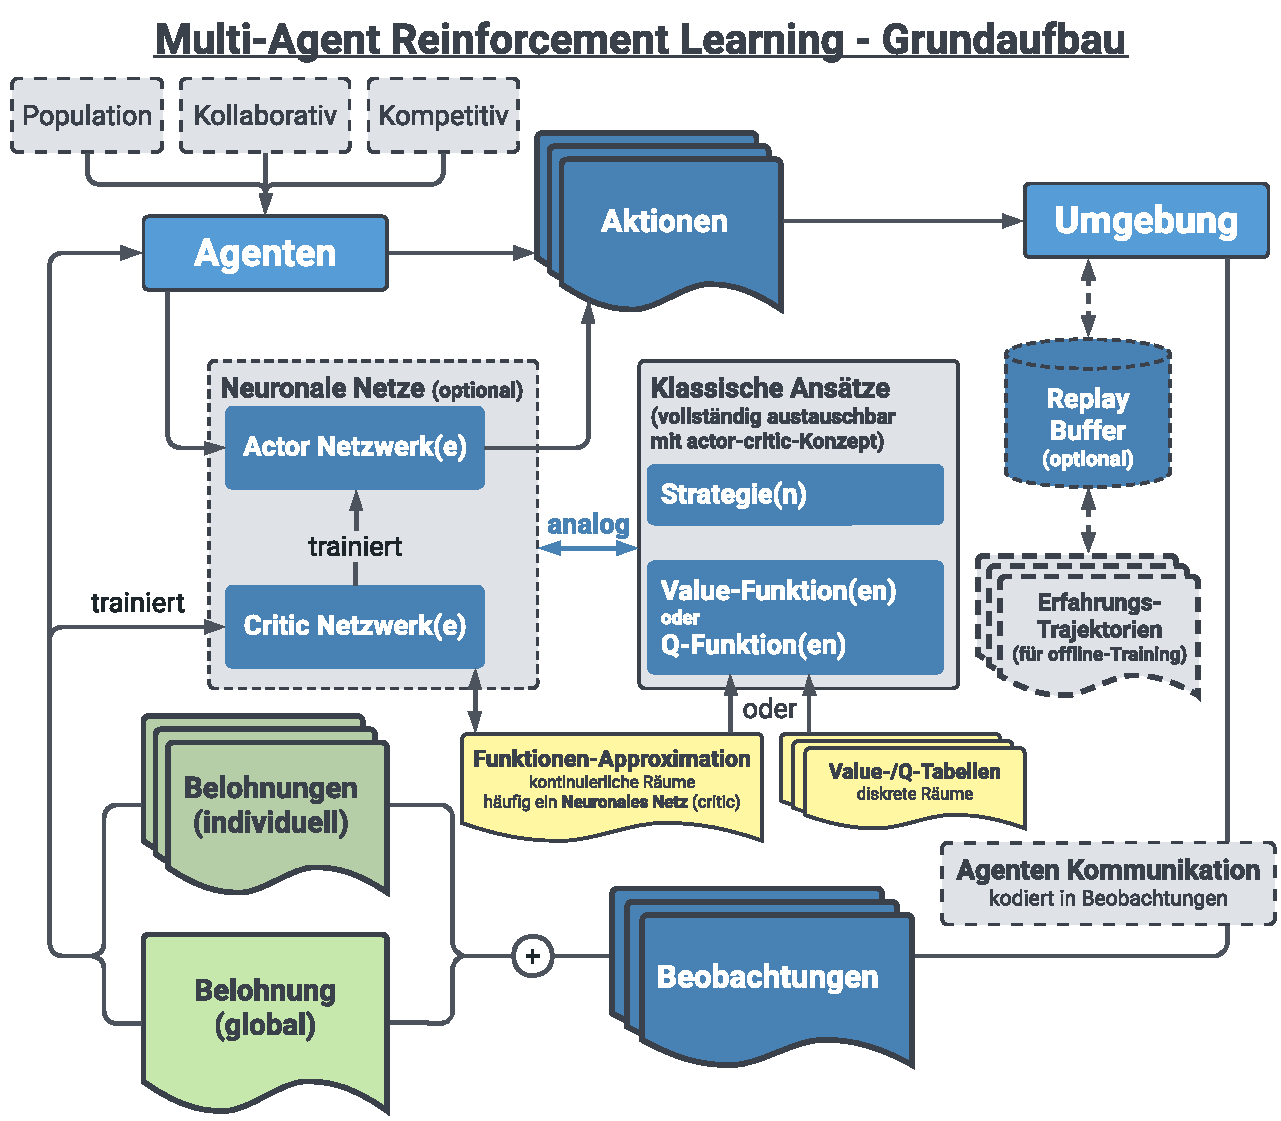
\includegraphics[width=.9\textwidth]{illustrations/MARL_Grundaufbau.pdf}
    \caption{Grundlegendes Konzept des Multi-Agent Reinforcement Learnings.}
    \label{fig:MARL_Konzept}
\end{figure}

\textbf{Fragestellungen}

Bei der Erweiterung auf ein MA System ergeben sich neue Möglichkeiten und damit auch neue Fragen, die individuell für ein vorliegendes Problem beantwortet werden müssen. Für diese Arbeit relevante Fragen sind bspw.: Gibt es eine zentrale Steuerung oder sind alle Agenten autonom? Gibt es verschiedene Populationen von Agenten (heterogene Parameter-Verteilung)? Gibt es mehrere Strategien, also unterschiedliche Ziele? Was sehen die Agenten; teilen sie Informationen? Wie werden Belohnungen in einem Multi-Agenten-System verteilt oder zugewiesen (lokale vs. globale Belohnungen)? \\

In dieser Arbeit wird konzeptionell alles so einfach und direkt wie möglich gehalten. Daher können all diese Fragen sofort adressiert werden:

\begin{task}[MARL-Umsetzung in dieser Arbeit]
    Jedes Teilchen soll autonom handeln, aber dieselbe Strategie teilen. Alle Agenten optimieren also gemeinsam dieselbe Strategie (\textit{shared policy}). Es gibt nur eine Population und die Agenten haben nur lokale Informationen. Die Belohnung jedoch entspricht der globalen Änderung des Ordnungsparameters. Die Alternative dazu wäre, dass die Agenten nur den Ordnungsparameter ihrer Gruppe sehen und optimieren. Dann entspricht die Belohnung aber nicht mehr der Maximierung des globalen Ordnungsparameters, wie es das Vicsek-Modell versucht.
\end{task}

\textbf{Verfügbare Frameworks für (MA)RL}

Verschiedene Frameworks bieten bereits implementierte Algorithmen und Strukturen, die die Entwicklungszeit erheblich reduzieren können. Sie implementieren die in diesem Abschnitt beschriebenen algorithmischen Grundlagen und bieten sowohl eine breite Palette an voreingestellten Konfigurationen als auch umfangreiche Optionen zur individuellen Anpassung. Zu den bekanntesten zählen OpenAI's \texttt{Gym} (in neuen Versionen \texttt{Gymnasium}) für Reinforcement Learning \cite{OpenAiGym}, Ray's \texttt{RLlib} für skalierbare RL- und MARL-Implementierungen \cite{RLlib} (\textbf{\textit{wird in dieser Arbeit verwendet}}), und TensorFlow Agents (\texttt{TF-Agents}) \cite{TFAgents}, eine zuverlässige Bibliothek für komplexe RL-Probleme (kein Multi-Agent).\\

Nachdem mit MARL eine eher konzeptionelle Erweiterung des Reinforcement Learnings vorgestellt wurde, stellt sich nun die Frage nach einer konkreten Trainings- und Optimierungsstrategie. Einige gängige Methoden werden im nächsten Abschnitt skizziert.

\subsection*{Proximal Policy Optimization (PPO)}

Proximal Policy Optimization (PPO) ist einer der führenden Algorithmen im Bereich des Reinforcement Learnings. Obwohl zahlreiche Algorithmen für die Strategieoptimierung existieren, hat sich PPO als besonders effektiv und stabil erwiesen \cite{schulman2017ppo}. Die Entscheidung für einen bestimmten Algorithmus hängt von verschiedenen Faktoren ab, insbesondere aber von der Beschaffenheit der Umgebung (kontinuierlicher vs. diskreter Aktions- und Zustandsraum).\\

\textbf{Übersicht über Algorithmen im Reinforcement Learning}

Für ein besseres Verständnis der Auswahlmöglichkeiten und der Position von PPO im Spektrum der RL-Algorithmen dienen die Abbildungen \ref{fig:RL_Algorithms} und \ref{fig:Algorithms_Venn}. Weit verbreitete kontinuierliche Algorithmen sind PPO, SAC (Soft Actor-Critic) \cite{SAC} und DDPG (Deep Deterministic Policy Gradients) \cite{DDPG}, während für den diskreten Raum Algorithmen wie Q-Learning \cite{QLearning1992} und DQN (Deep Q-Networks) \cite{DQN2013} populär sind.

All die aufgelisteten Algorithmen können auf Multi-Agent Systeme erweitert werden.

\begin{figure}[h!]
    \centering
    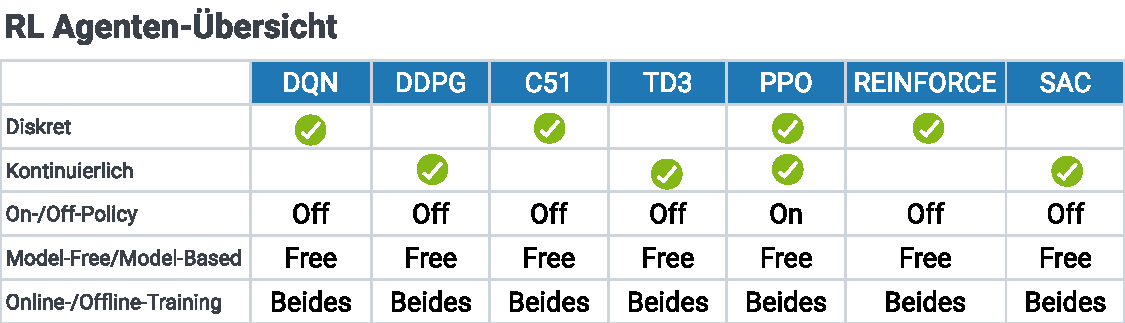
\includegraphics[width=.9\textwidth]{illustrations/RL_Algorithms.pdf}
    \caption{Übersicht der zurzeit meist verwendetsten Reinforcement Learning Algorithmen.}
    \label{fig:RL_Algorithms}
\end{figure}

\divider

\textbf{Terminologie und Klassifizierung}

Für das Verständnis der Algorithmen werden 3 bzw. 6 weitere Begriffe erklärt. Diese können tendenziell der Tabelle \ref{tab:RL_basic_terms} zugeordnet werden, sind aber im Kontext konkreter Algorithmen besser zu verstehen.

\begin{itemize}
    \item \textit{On-Policy vs. Off-Policy}: On-Policy-Algorithmen wie PPO aktualisieren die Strategie basierend auf den Daten der aktuellen Strategie. Off-Policy-Algorithmen wie DQN können Daten aus vorherigen Strategien verwenden.
    \item \textit{Model-Free vs. Model-Based}: Model-Based-Algorithmen lernen und simulieren die Dynamik der Umgebung zur Optimierung zukünftiger Entscheidungen. Im Gegensatz dazu benötigen Model-Free-Algorithmen wie PPO und DQN kein solches Umgebungsmodell, sondern lernen direkt durch Interaktion.
    \item \textit{Online vs. Offline Training}: Beim Online-Training werden Daten in Echtzeit gesammelt und verarbeitet. Beim Offline-Training wird ein Datensatz gesammelt und dann zur Optimierung verwendet.
    \item \textit{Exploration vs. Exploitation}: Exploration-Exploitation-Strategien regeln die Balance zwischen der Erkundung neuer Aktionen und der Ausführung bekannter, belohnungsoptimaler Aktionen. Algorithmen wie PPO können mithilfe von Methoden wie dem Epsilon-Greedy-Ansatz oder der Boltzmann-Exploration modifiziert werden, um eine geeignete Trade-off-Strategie zu ermöglichen.
\end{itemize}

\divider

\begin{figure}[h!]
    \centering
    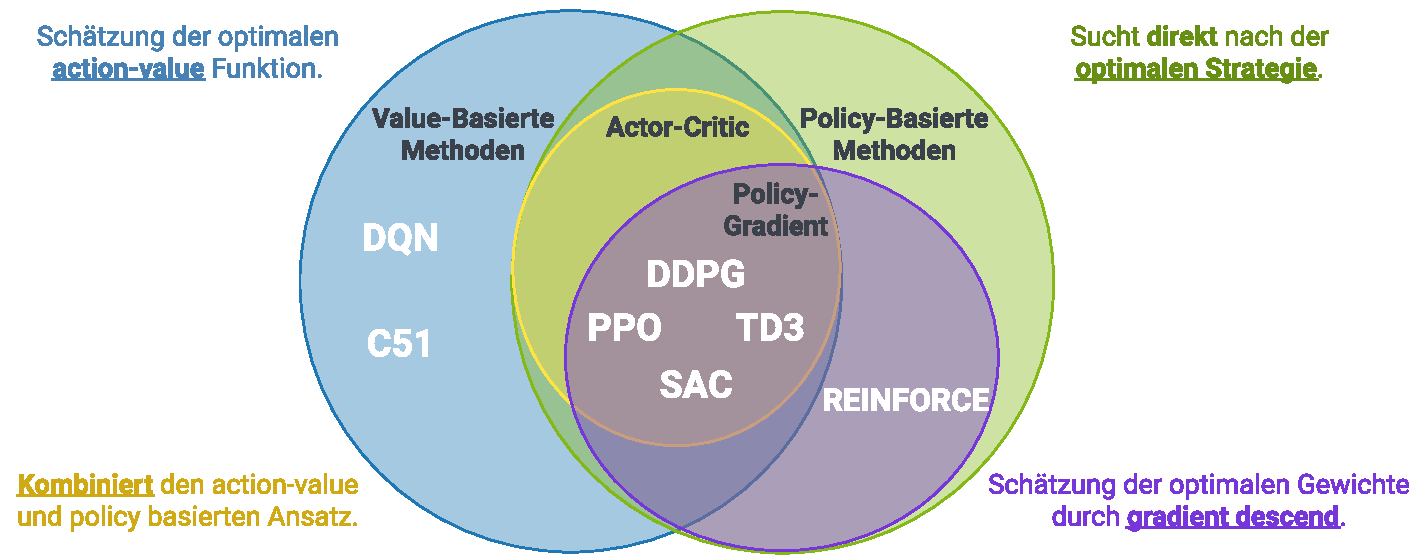
\includegraphics[width=.9\textwidth]{illustrations/Algorithms_Venn.pdf}
    \caption{Klassifizierung gängiger Reinforcement-Learning-Algorithmen nach ihrer Herangehensweise: Value-Based, Policy-Based und Policy Gradient Methoden, inklusive der speziellen Actor-Critic-Techniken, die Elemente aus verschiedenen Kategorien kombinieren und häufig neuronale Netze verwenden.}
    \label{fig:Algorithms_Venn}
\end{figure}

\begin{task}[Warum PPO?]
    PPO überzeugt durch seine Robustheit und Effizienz. Als moderner Algorithmus baut er auf bewährten Konzepten auf und hat sich in vielen Bereichen bewiesen. Zudem kann er sowohl mit diskreten, als auch mit kontinuierlichen Aktions- und Zustandsräumen arbeiten. Daher wird dieser Algorithmus häufig als Standard angesehen, insbesondere für MARL-Aufgaben. Durch seine Beliebtheit ist PPO mit vielen Beispielen belegt und gut dokumentiert, was durch die starke Entwicklung in diesem Bereich durchaus relevant ist. Im Kern von PPO steht das Training eines neuronalen Netzes, was diesen Algorithmus für die Aufgabe dieser Arbeit qualifiziert.
\end{task}

\newpage

\textbf{Mathematischer Kern von PPO}

PPO optimiert eine Wahrscheinlichkeitsverhältnisfunktion:

$$\pi_{\theta}(a_t|s_t) / \pi_{\theta_{\text{alt}}}(a_t|s_t)$$

In diesem Ausdruck bezeichnet \( \pi_{\theta}(a_t|s_t) \) die Wahrscheinlichkeit der Aktion \(a_t\) im Zustand \(s_t\) gemäß der aktuellen Politik mit Parametern \(\theta\). \( \pi_{\theta_{\text{alt}}}(a_t|s_t) \) ist die Wahrscheinlichkeit derselben Aktion im selben Zustand, jedoch gemäß der vorherigen Politik.

Die optimierte Funktion wird geclippt, um die Aktualisierung der Politik zu stabilisieren:

\[
\text{min} \left( r_t(\theta) \hat{A}_t, \text{clip}(r_t(\theta), 1 - \epsilon, 1 + \epsilon) \hat{A}_t \right)
\]

Hierbei ist \( \hat{A}_t \) der geschätzte Vorteil der Aktion \( a_t \), definiert als:

\[
\hat{A}_t = Q(s_t, a_t) - V(s_t)
\]

\( Q(s_t, a_t) \) ist der erwartete zukünftige Ertrag der Aktion \( a_t \) im Zustand \( s_t \), und \( V(s_t) \) ist der Wert des Zustands \( s_t \) gemäß der aktuellen Politik.

Der Vorteil \( \hat{A}_t \) ist ein zentrales Element von Actor-Critic-Ansätzen. Er zeigt an, wie viel besser oder schlechter eine Aktion im Vergleich zu anderen möglichen Aktionen im gleichen Zustand ist. Dadurch wird eine effizientere Optimierung der Politik ermöglicht.

\newpage
\section{Nachbildung bestehender Modelle}
\label{sec:Nachbildung}
Bevor Maschinelles Lernen auf eine Schwarmsimulation angewendet werden kann, muss eine Simulation basierend auf einem Modell implementiert und validiert werden. Dieses Kapitel behandelt die Implementierung der Simulation und untersucht sowohl das Vicsek-Modell als auch andere Modell-Familien. Zur Bewertung der Implementierungsgenauigkeit erfolgt ein Vergleich der Simulationsergebnisse mit Ergebnissen aus vorhandenen Studien. Gleichzeitig werden die hier verwendeten statistischen Methoden auf ihre Robustheit überprüft.

\subsection{Methodologie der Simulation}
Die Konzeption der Simulation gliedert sich in drei aufeinanderfolgende Phasen: Die Auswahl der Software und Strukturierung der Implementierung; die Anwendung spezifischer Programmiertechniken zur Lösung besonderer Aufgaben; und letztlich die zuvor erwähnte Validierung der Ergebnisse durch Vergleich und statistischen Methoden.\\

\textbf{Wahl der Software: \texttt{C++} und \texttt{Python}}

Für diese Arbeit werden die Programmiersprachen \texttt{C++} \cite{cpp14} und \texttt{Python}\footnote{Programmiersprache im allgemeinen Verständnis, Skriptsprache im spezifischeren Kontext.} \cite{python310} verwendet. Diese Wahl liegt in den einzelnen Stärken und der Synergie beider Sprachen begründet.

\texttt{C++} ist als moderner Standard und vor allem wegen seiner Effizienz besonders geeignet. Eine Vielteilchensimulation kann selbst bei einfachen Wechselwirkungen schnell einen beachtlichen Rechenaufwand fordern. Eine Simulation mit $N \geq \num{10000}$ Teilchen, wie Vicsek \textit{et al.} sie untersucht haben, kann dann nur mit ausreichend effizienten Methoden praktisch untersucht werden.

\texttt{Python} ist insofern eine natürliche Ergänzung zu \texttt{C++}, als dass es nicht nur mit seinen eigenen Stärken überzeugt, sondern auch eine effektive Schnittstelle für \texttt{C++} bietet.

Auswahlkriterien zusammengefasst:

\begin{enumerate}
    \item \textbf{Stärken von \texttt{Python}}: Schnelles Prototyping, einfaches Visualisieren (\texttt{Matplotlib}), schnelles Debugging, hohe Funktionalität. Dadurch auch: Visuelles Debugging einfach möglich.
    \item \texttt{pybind11}\cite{pybind11}: Einbinden von eigenem \texttt{C++11} Code/Funktionen in \texttt{Python}.
    \item \textbf{Maschinelles Lernen}: \texttt{Python} ist die bevorzugte Sprache für Maschinelles Lernen, da viele einschlägige Bibliotheken, einschließlich der in dieser Arbeit verwendeten \texttt{TensorFlow}- und \texttt{RLlib}-Bibliothek, speziell und oft exklusiv für \texttt{Python} entwickelt wurden.
\end{enumerate}

Häufig ist es von Interesse, das System zur Überprüfung zu visualisieren. Um vor allem große Simulationen performant visualisieren zu können, kann die Software \texttt{Ovito} \cite{OVITO2010} verwendet werden. Diese Software wird in der Festkörperphysik verwendet und dient hauptsächlich der Visualisierung von atomaren und molekularen Strukturen, sowie der Darstellung ihrer dynamischen Eigenschaften über die Zeit. Sie eignet sich für diesen Fall aber auch für die einfache Darstellung von zeitaufgelösten Teilchenpositionen und besonders für sehr große Teilchenzahlen (bis etwa $N = \num{100000}$) in Echtzeit, indem alle Teilchenpositionen für jeden Zeitschritt in eine \texttt{.xyz}-Datei geschrieben werden. Die Dateien können je nach Länge der Simulation und Teilchenanzahl entsprechend groß werden, sind aber meistens noch im \texttt{MB}- bis \texttt{GB}-Bereich.\\

\textbf{Umsetzung der Simulation}

Die in dieser Arbeit entwickelte Simulation kann auf einige wenige Schwerpunkte reduziert werden. Wird von Beginn an eine objektorientierte Methodik angewendet, erleichtert dies die Strukturierung der Implementierung maßgeblich. Ein schematischer Projektaufbau, der die komplementäre Verwendung von \texttt{Python} und \texttt{C++} zeigt, befindet sich im Anhang (siehe Abbildung \ref{fig:SchematischerProjektaufbau}). \\

Die relevantesten Algorithmen sind in folgender Liste zusammengefasst:

\begin{task}[Die wichtigsten Aufgaben der Simulation]
\begin{multicols}{2}
    \begin{itemize}[left=0em, itemsep=0em, topsep=0em, parsep=0em]
        \item {\fontsize{11}{14}\selectfont \textbf{Zellenaufteilung und Teilchenzuweisung}}

        \;\;\textbf{\textit{Ziel}:} Reduktion des Rechenaufwands.
        
        \;\;\textbf{\textit{Komplexität}:} Hoch, da fehleranfällig. Es müssen Randeffekte berücksichtigt werden.\\
        
        \item {\fontsize{11}{14}\selectfont \textbf{Nachbarschaftslisten und -Bestimmung}}

        \;\;\textbf{\textit{Ziel}:} Hier: Bereitstellung der Nachbarn für die Modell-Regeln. Können auch verwendet werden, um den Rechenaufwand zu reduzieren.
        
        \;\;\textbf{\textit{Komplexität}:} Mittel/Hoch, entsprechend den beiden genannten Zielen. Die Wahl von performanten Methoden (Sortierung, Zufallsgenerator, Distanzbestimmung) hat hier einen großen Einfluss. Durch diese Aufgabe sind topologische Modelle wesentlich rechenintensiver als metrische Modelle.
        
        \item {\fontsize{11}{14}\selectfont \textbf{Periodische Randbedingungen}}

        \;\;\textbf{\textit{Ziel}:} Simulation eines unendlich ausgedehnten Systems.
        
        \;\;\textbf{\textit{Komplexität}:} Gering, aber fehleranfällig, da diese Bedingungen auf mehreren Ebenen berücksichtigt werden müssen (Distanzbestimmung).\\
        
        \item {\fontsize{11}{14}\selectfont \textbf{Gleichzeitigkeit}}

        \;\;\textbf{\textit{Ziel}:} Sicherstellung, dass alle Teilchen gleichzeitig aktualisiert werden.
        
        \;\;\textbf{\textit{Komplexität}:} Leicht bis Mittel. Die Komplexität liegt in der Natur von \texttt{C++} und dem Verwenden von Parallelisierungen.\\
        \;\\
    \end{itemize}
\end{multicols}
\end{task}


Von all diesen Aufgaben steht das Bestimmen der Nachbarn im algorithmischen Kern der Simulation. Diese Berechnung ist am kostenintensivsten und fehleranfälligsten; nicht zuletzt, weil dies die einzige Aufgabe ist, die sich zu parallelisieren lohnt. Um einen quadratischen Rechenaufwand $\mathcal{O}(n^2)$ zu vermeiden, wird der Simulationsbereich in quadratische \textbf{Zellen} aufgeteilt, die in ihrer Kantenlänge dem Wechselwirkungs-Durchmesser $2r$ entsprechen. Die Teilchen werden dann den entsprechenden Zellen zugeordnet. Dies ermöglicht die Untersuchung einer kleinen Nachbarschaft an Zellen, statt über jedes einzelne Teilchen iterieren zu müssen.\\

Für eine Aufteilung der Simulation in Zellen oder gar dem geschickten Verwalten von Adjazenzlisten gibt es auch fortgeschrittene und effektivere Methoden, wie etwa \texttt{Verlet-Listen} \cite{VerletListe} oder \texttt{Quadtrees} \cite{Quadtree}, die eine dynamische Anpassung der Zellen ermöglichen und den Rechenaufwand weiter minimieren. Diese Methoden wurden jedoch aus Komplexitäts- und Implementierungsgründen in dieser Arbeit nicht verfolgt.\\

Weitere Herausforderungen und typische Probleme der Implementierung waren - neben den 4 gelisteten Aufgaben - die Fehleranfälligkeit von Randfällen, die Sensibilität von \texttt{C++} Parallelisierungen, die notwendige Kompromissbereitschaft bei Zufallsgeneratoren und das Optimieren rechenintensiver Operationen wie etwa das Sortieren oder das Mischen von Vektoren.

Zur Validierung der Implementation wurden die Simulationen mit zahlreichen Details und Informationen visualisiert. Abbildung \ref{fig:VisuellesDebugging} zeigt eine Simulation mit einem üblichen Randfall. Diese visuelle Stütze war für die Entwicklung der Simulation unverzichtbar.


\subsection{Vicsek-Modell und topologisches Modell}
Das Vicsek-Modell und das topologische Modell dienen als Grundlage für die Analyse der Schwarmdynamik in dieser Arbeit. Um die Qualität der Simulation zu überprüfen, werden die Messergebnisse mit bereits vorhandenen Forschungsergebnissen abgeglichen. Außerdem werden einfache statistische Methoden angewendet, um die Messstabilität weiter zu verbessern.

\subsection*{Statistische Methoden zur Optimierung der Messgenauigkeit}
Die für die gesamte Auswertung relevante Größe ist der Ordnungsparameter $v_a$ \eqref{eq:ordnungsparameter_vicsek}. Das Ziel ist die Equilibrierung einer Simulation eines spezifischen Parametersatzes. Für jeden Zeitschritt in der Simulation kann der Ordnungsparameter berechnet werden. Der na\"ive Ansatz, am Ende einer langen Simulation den finalen Wert für $v_a$ abzugreifen, wird kein zuverlässiges Ergebnis produzieren. Die Fluktuationen von $v_a$ können durch das Rauschen $\eta$ so stark sein, dass auch eine Mittelung über einige letzte Werte von $v_a$ nur in seltenen Fällen aussagekräftig ist.

Stattdessen werden einfache statistische Methoden angewendet, um nicht nur den Ordnungsparameter $v_a$ zuverlässig quantifizieren zu können, sondern auch um unnötig lange Simulationszeiten zu vermeiden.\\

%\textbf{Gesetz der großen Zahlen \& Zentraler Grenzwertsatz}

Das Rauschen $\eta$ bewirkt, dass der Ordnungsparameter $v_a$ auch im equilibrierten Zustand eines Systems eine zufallsverteilte Größe ist. In solchen Fällen garantiert das \textbf{Gesetz der großen Zahlen}, dass der Durchschnitt der Messreihe bei großen Stichproben gegen den Erwartungswert konvergiert. Wenn die Zufallszahlen zudem \textbf{unabhängig} voneinander sind, ist auch der \textbf{Zentrale Grenzwertsatz} gültig. Dadurch sinkt der Fehler der Messreihe proportional zu $\tfrac{1}{\sqrt{T}}$, und die Verteilung der Messdaten um den Erwartungswert kann als normalverteilt betrachtet werden. $T$ entspricht hier der Anzahl der Zeitschritte und damit der Anzahl der Messwerte.\\

\textbf{Autokorrelation}

Unabhängig von den Parametern einer Simulation werden direkt aufeinanderfolgende Messungen miteinander korreliert sein. Um diese Korrelation aufzuheben, kann die Korrelationszeit $\tau_c$ bestimmt und verwendet werden. Messungen, die nur alle $\tau_c$ Simulationsschritte durchgeführt werden, sind damit nicht mehr oder nur wenig korreliert. Das Aufheben der Korrelation ist wünschenswert, da es die Proportionalität der Fehlerabschätzung von $\tfrac{1}{\sqrt{T}}$ gewährleistet, indem die Messungen statistisch unabhängig voneinander gemacht werden.

Das Bestimmen der Autokorrelationszeit ist jedoch aufwendig, da sie für jede einzelne Parameterkonfiguration bestimmt werden muss. In diesem Sinne müsste auch ihre Wiederverwendbarkeit getestet werden. Obwohl die Autokorrelationszeit durchaus relevant und hilfreich ist, werden für das dynamische Beenden einer Simulation andere Methoden verwendet.\\

\textbf{Konvergenzkriterien und Stabilität}

Um die zuvor motivierten Theoreme anwenden zu können, ohne die Autokorrelationszeit zur Gewährleistung der statistischen Unabhängigkeit bestimmen zu müssen, werden aufeinanderfolgende Messungen in \textbf{Sweeps} durchgeführt. Im Optimalfall entspricht die Länge bzw. Größe eines Sweeps der Autokorrelationszeit. Da diese nicht bekannt ist, wird die Länge eines Sweeps auf die Teilchenzahl $N$ gesetzt. Diese na\"ive Strategie hat sich bereits im Ising-Modell als effektiv erwiesen \cite{Ising1925}. Zwar wird damit keine Unabhängigkeit garantiert; der nachteilige Effekt der Korrelation aber sicherlich abgefedert.

Als \textbf{Abbruchkriterium} wird ein \textbf{laufender Durchschnitt} verwendet. Nach einer \textbf{Burn-In Phase} von $\num{10}$ Sweeps beginnt die kumulative Summation des Ordnungsparameters. Fällt die \textit{absolute} Änderung des laufenden Durchschnitts unter eine Schranke von $\num{e-4}$ in $\num{10}$ aufeinanderfolgenden Messungen, wird das System als equilibriert angesehen und die Simulation beendet. Das Verwenden von mehreren Messungen verhindert, dass zwei konsekutive laufende Durchschnitte zufällig nah beieinander liegen. Die Burn-In Phase reduziert den Einfluss verschiedener Anfangsbedingungen. Als obere Schranke für die Simulationslänge dient eine empirisch bestimmte Grenze von $\num{750000}$ Zeitschritten, was im individuellen Fall $T = \tfrac{\num{750000}}{N}$ Messungen bzw. Sweeps entspricht.

Diese Herangehensweise hat sich als effizient und robust erwiesen und bietet einen pragmatischen Kompromiss zwischen methodischer Einfachheit und statistischer Zuverlässigkeit.

\subsection*{Vicsek-Modell}
\label{sec:Vicsek_Modell_Analytisch}

Die Simulationsergebnisse für das Vicsek-Modell sind in je zwei vergleichenden Abbildungen gegenübergestellt. Abbildung \ref{fig:Topologisch_1a} zeigt die klassische Untersuchung eines Schwarms bei Variation des Rauschens $\eta$. Dieser Plot gibt Aufschluss darüber, wie stabil ein Schwarm bei entsprechendem Rauschen ist. Es ist erkennbar, dass Systeme mit größerem Simulationsbereich mehr Unordnung aufweisen. Da alle Simulationen bei gleicher Dichte $\rho = 4$ durchgeführt wurden, kann daraus abgeleitet werden, dass es eine \textbf{effektive Wechselwirkungsreichweite} gibt. Die Überlegung dazu ist intuitiv: Es gebe ein Teilchen A, das ein anderes Teilchen B am Rand seines Wechselwirkungsradius $r$ sieht. Teilchen B sehe nun ein weiteres Teilchen C, das jedoch entgegengesetzt zu A positioniert ist. Damit wechselwirkt Teilchen A indirekt mit Teilchen C über Teilchen B (siehe Abbildung \ref{fig:EffektiverWWRadius}). Für die Propagation von A zu C ist jedoch ein Simulationsschritt notwendig. Bei maximalem Abstand gilt die Regel, dass eine Wechselwirkung $\const{n}$-ter Ordnung $\const{n}$ Simulationsschritte benötigt, um zu propagieren. In den Simulationen wird diese Propagation durch das Rauschen $\eta$ gestört. Bei zu starkem Rauschen gehen die Informationen in dem stochastischen Störfaktor verloren. Daher ist es plausibel, dass für gleichbleibende Dichte große Systeme instabiler sind; insbesondere bei hohem Rauschen.\\

Der Vergleich der ersten Ergebnisse zeigt eine gute Übereinstimmung mit den originalen Daten. Die Messkurven stimmen vor allem qualitativ überein. Bei genauerer Betrachtung liegen dennoch Abweichungen vor. Diese werden in dem Schluss-Teil \ref{sec:Diskussion} diskutiert.

\begin{figure}[h!]
    \centering
    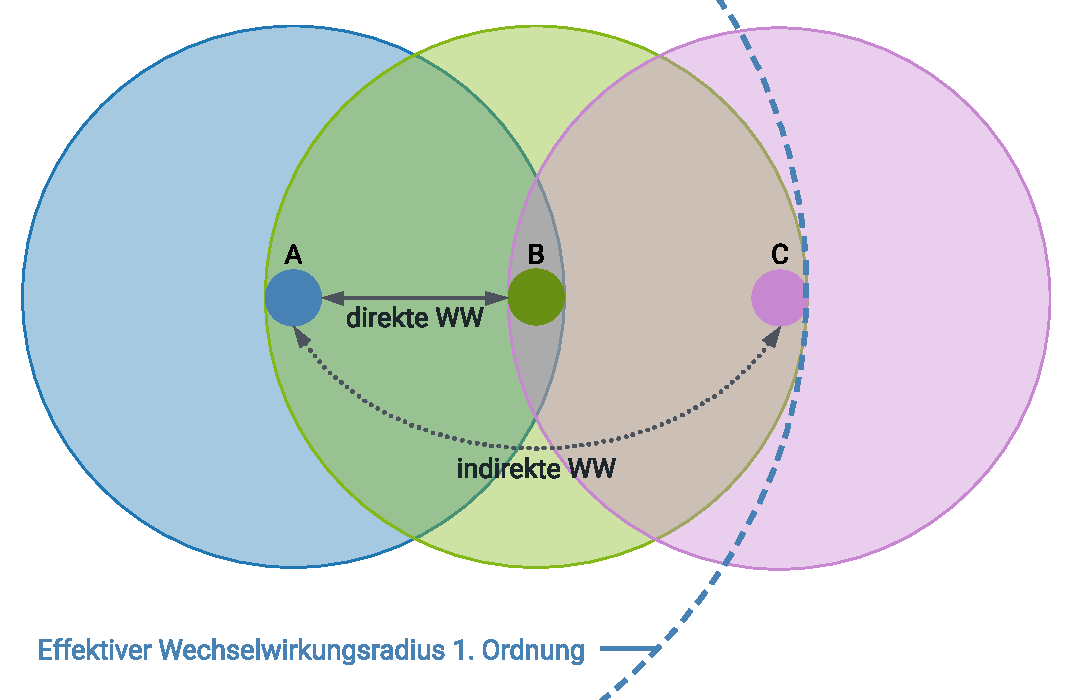
\includegraphics[width=.6\textwidth]{illustrations/EffektiverWWRadius.pdf}
    \caption{Effektiver Wechselwirkungsradius 1. Ordnung bei maximalem Abstand. Teilchen A und Teilchen C wechselwirken indirekt über Teilchen B.}
    \label{fig:EffektiverWWRadius}
\end{figure}

In dem zweiten Vergleich (Abbildung \ref{fig:Vicsek_1b}) wird nun die Dichte bei gleichbleibendem Rauschen variiert. Die durchgezogene Kurve in dem originalen Plot entspricht den kritischen \textit{Temperaturen} des Systems. Analog zu thermodynamischen Systemen übernimmt hier das Rauschen $\eta$ die Rolle einer Temperatur. Die beiden Abbildungen stimmen qualitativ bis auf den niedrigeren Wertebereich von $\rho$ überein.

\begin{figure}[h!]
    \centering
    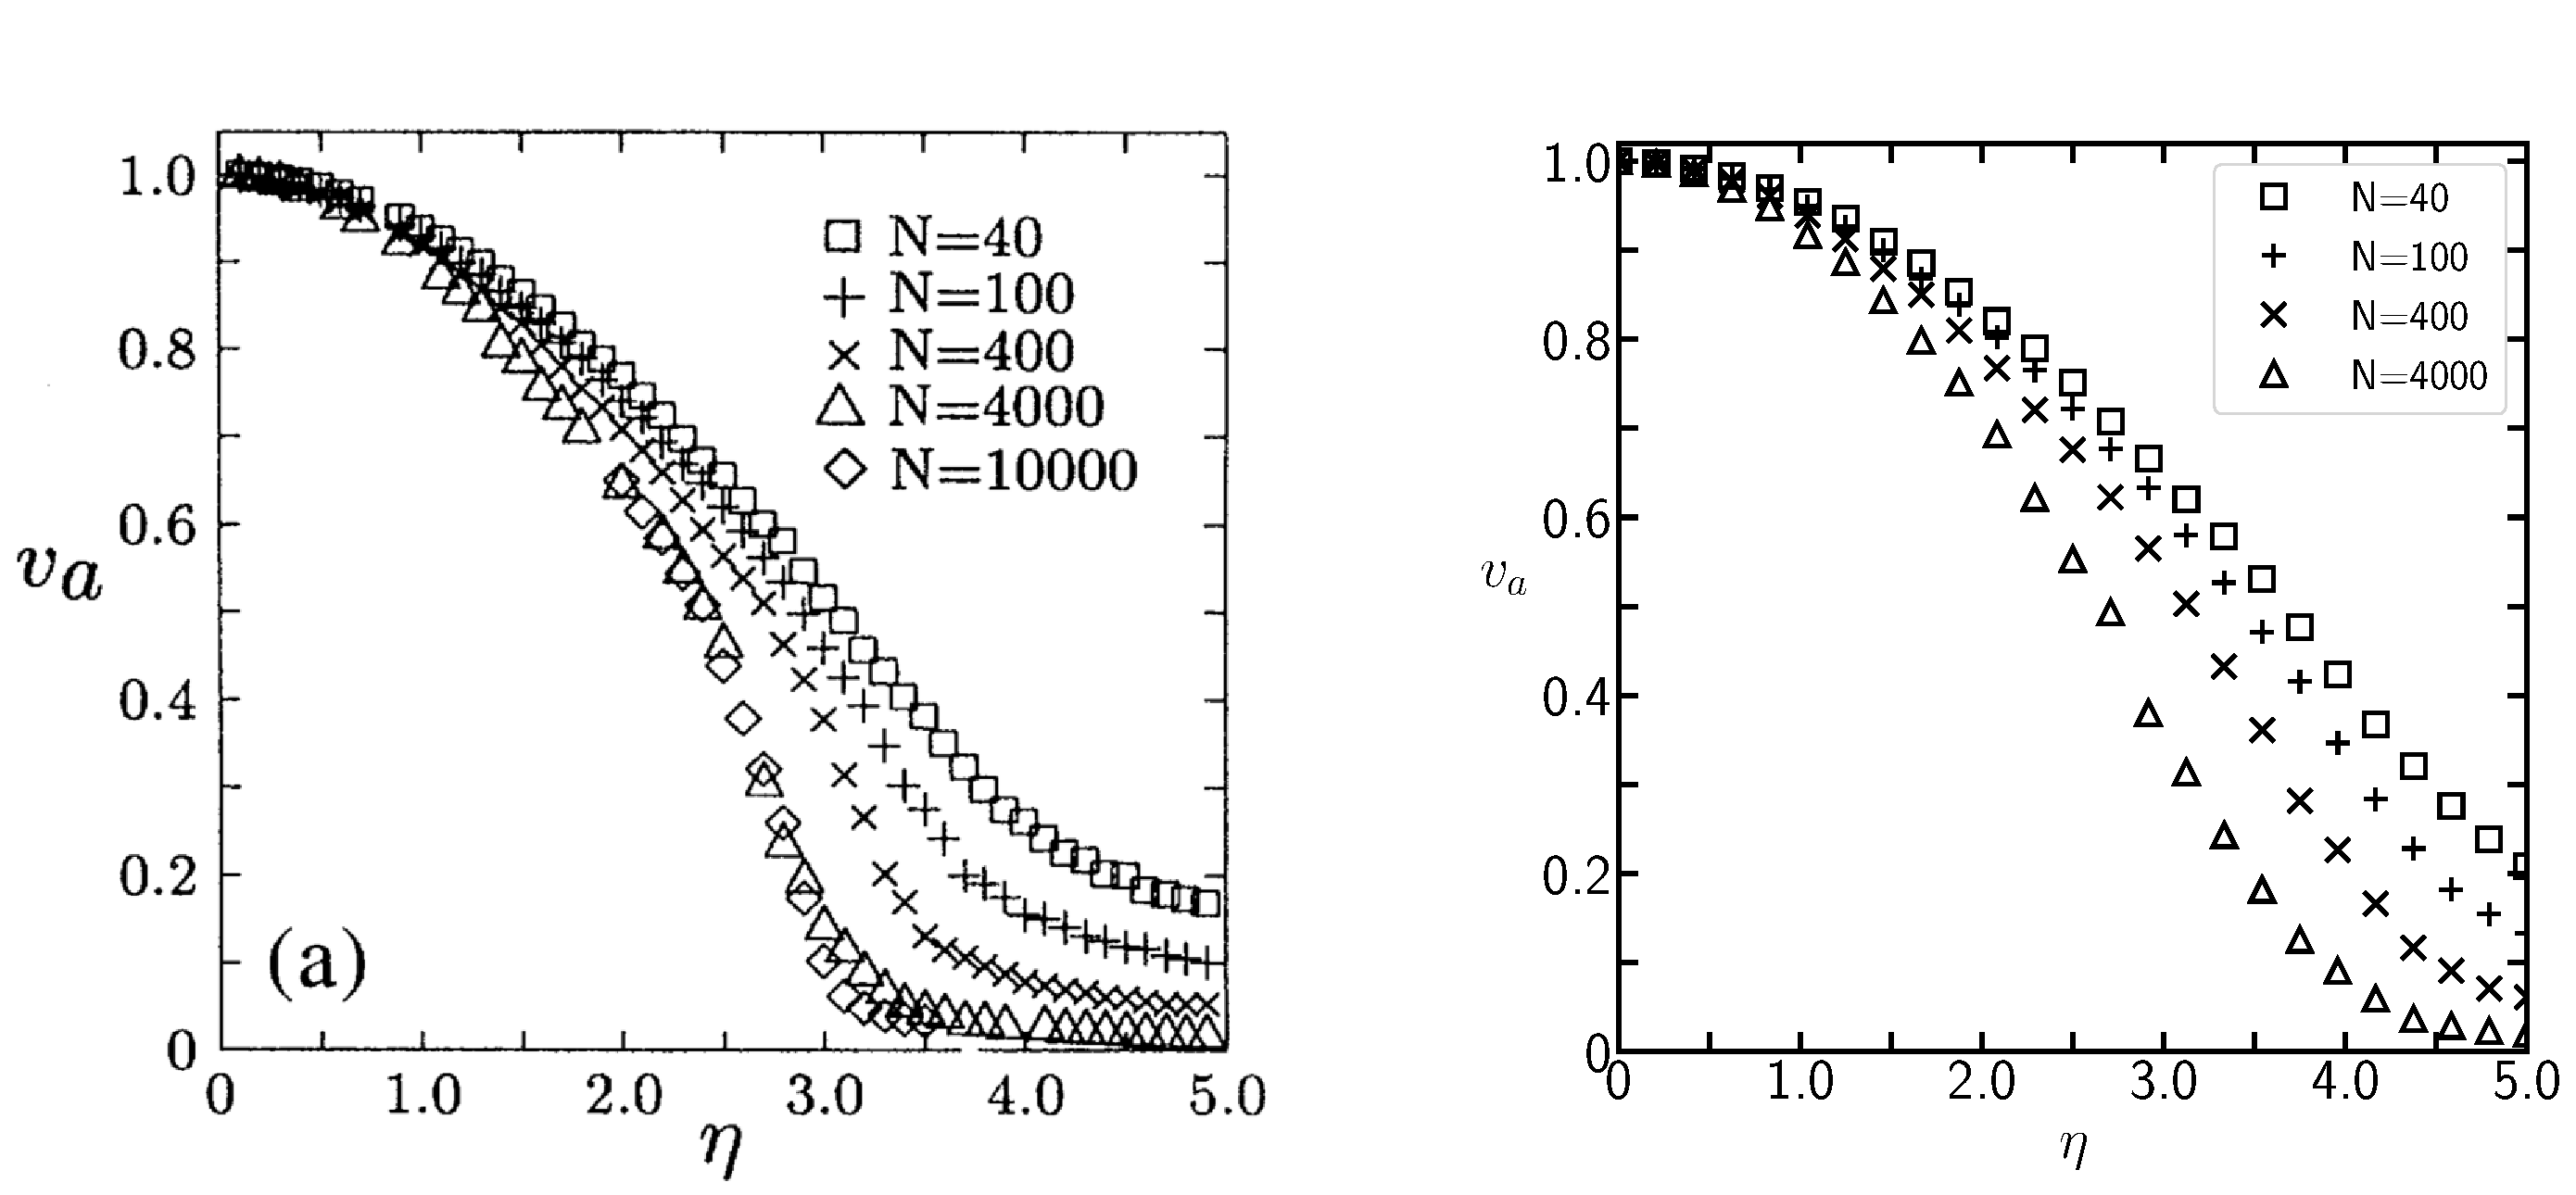
\includegraphics[width=.9\textwidth]{plots/Vicsek_1a_rRadius_final.pdf}
    \caption{\textbf{Links}: Messergebnisse aus der originalen Arbeit (Fig. 2a) \cite{vicsek1995}. \textbf{Rechts}: Messergebnisse der vorliegenden Implementierung. In beiden Abbildungen wurde $\rho = 4$ verwendet.}
    \label{fig:Vicsek_1a}
\end{figure}

\begin{figure}[h!]
    \centering
    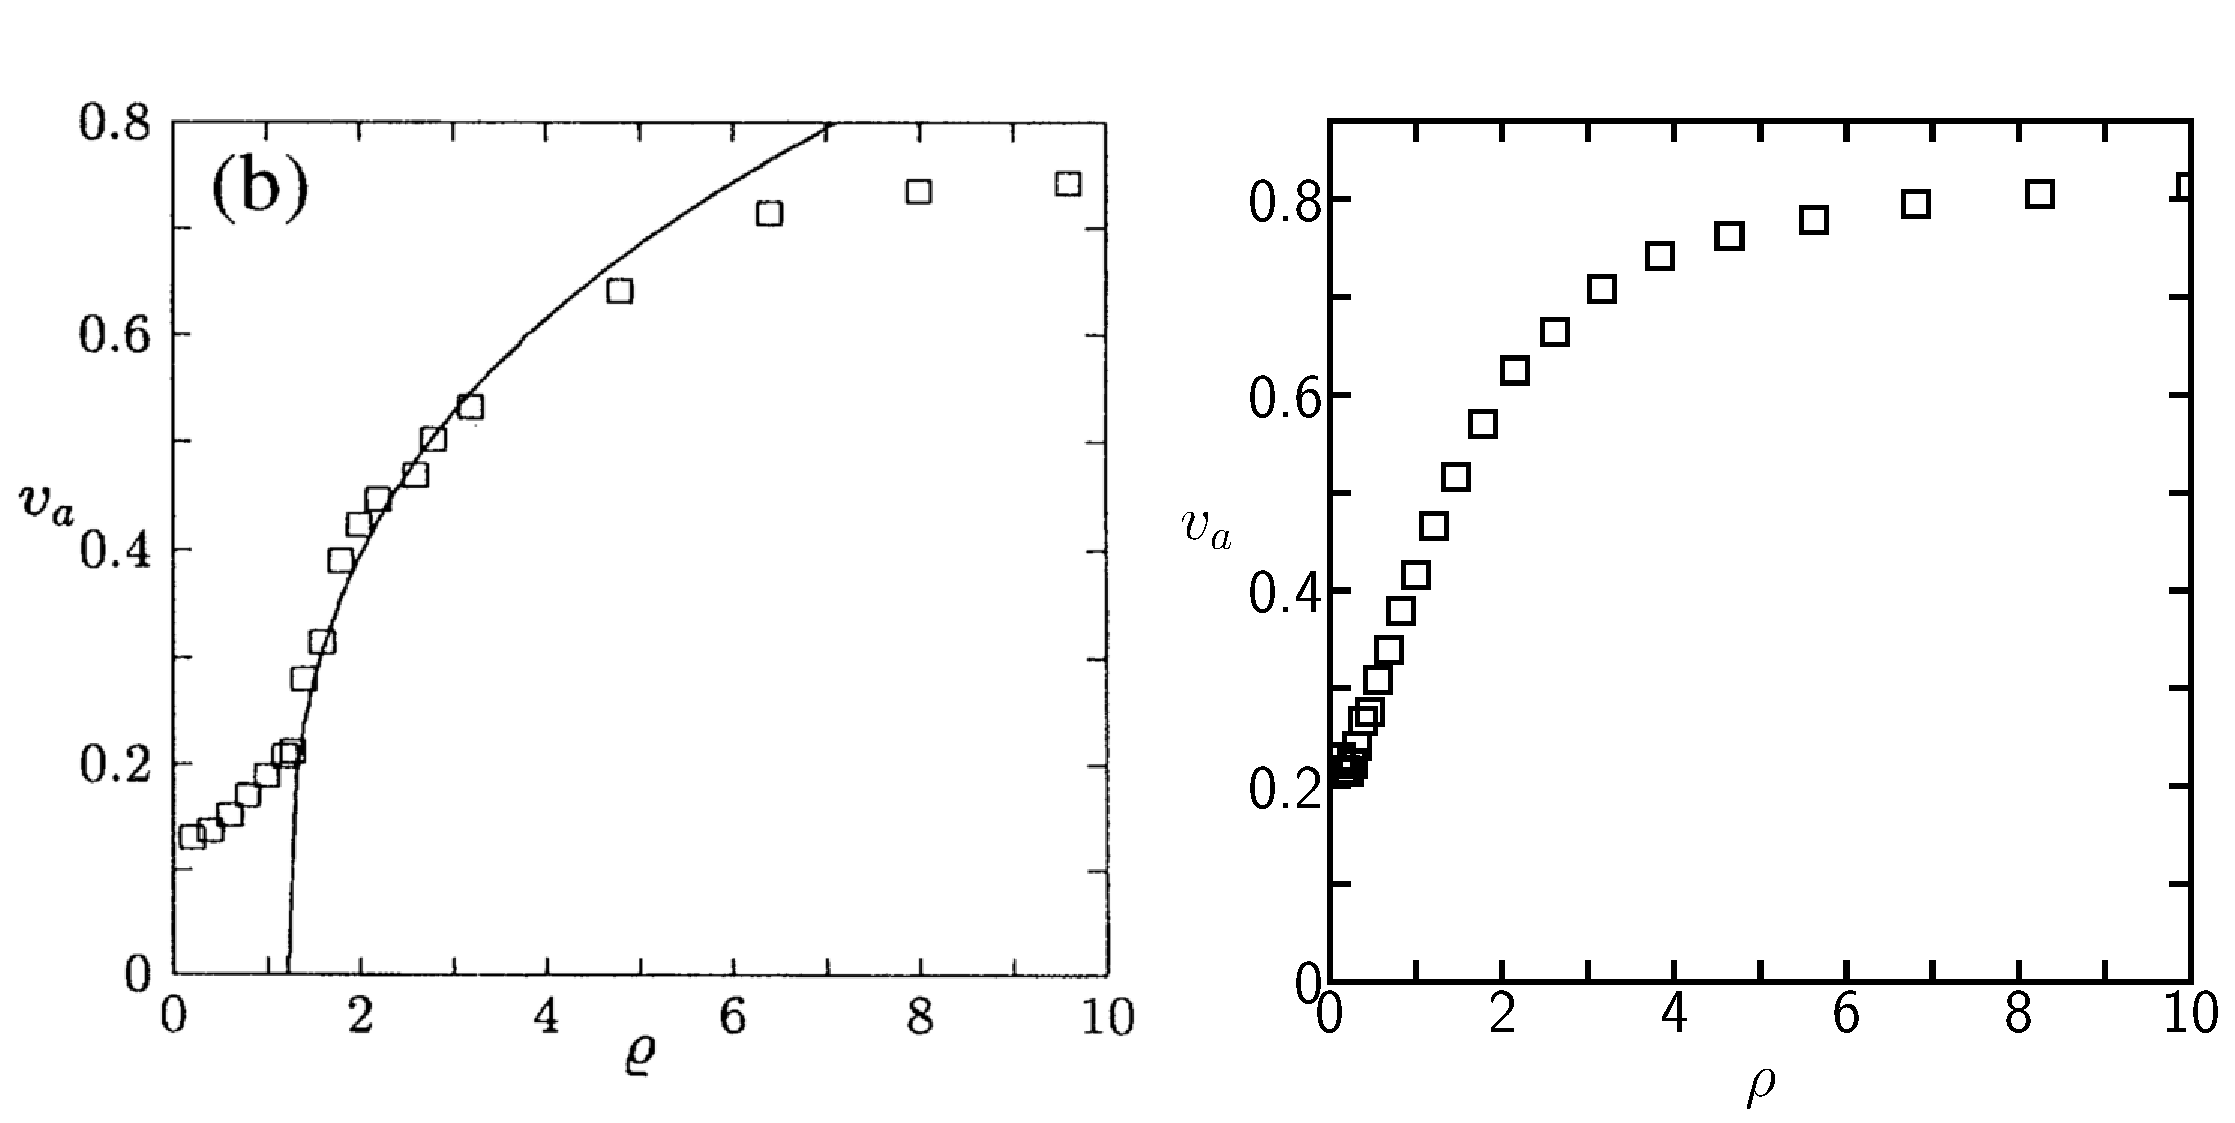
\includegraphics[width=.9\textwidth]{plots/Vicsek_1b_rRadius_final.pdf}
    \caption{\textbf{Links}: Messergebnisse aus der originalen Arbeit (Fig. 2b) \cite{vicsek1995} bei \textit{unbekanntem} Rauschen $\eta$. \textbf{Rechts}: Messergebnisse der vorliegenden Implementierung für $\eta = 2.0$. In beiden Abbildungen ist $L = 20$ konstant.}
    \label{fig:Vicsek_1b}
\end{figure}

\textbf{Analytische Untersuchungen}

Es kann gezeigt werden, dass die Ausrichtungsregel \eqref{eq:vicsek_rule} des Vicsek-Modells den Ordnungsparameter $v_a$ \eqref{eq:ordnungsparameter_vicsek_polar} minimiert. Hierfür wird der Ordnungsparameter in Polardarstellung gebracht und nach dem Winkel $\varphi_k$ abgeleitet. Die Überlieferung in die Polardarstellung produziert eine Wurzel:

\begin{equation}
    \begin{aligned}
        v_a &= \frac{1}{N v_0}\left|\sum_{i=0}^N \Tilde{\vec{v}}_i\right| = \frac{1}{N v_0}\left|\sum_{i=0}^N v_0\left(\begin{array}{c}
        \cos \varphi_i \\
        \sin \varphi_i
        \end{array}\right)\right| \\
        &= \frac{1}{Nv_0} \sqrt{v_0^2\left[\left(\sum_i^N \cos \varphi_i\right)^2+\left(\sum_i^N \sin \varphi_i\right)^2\right]}
    \end{aligned}
    \label{eq:ordnungsparameter_vicsek_polar}
\end{equation}

Um den Gebrauch der Kettenregel beim Ableiten der Wurzel zu vermeiden, wird $v_a$ quadriert. Dadurch ändern sich die Nullstellen der ersten Ableitung nicht, denn es gilt

$$\frac{\const{d}}{\const{d}x} \left(f(x)\right)^2=2 f(x) f^{\prime}(x) \quad .$$

Im Allgemeinen können weitere Nullstellen für $\frac{\const{d}}{\const{d}x} \left(f(x)\right)^2$ hinzukommen, und zwar für jedes $x_i$ mit $f(x_i) = 0$ und $f^{\prime}(x_i) \neq 0$. Der Ordnungsparameter $v_a$ ist zwar auf $v_a \in [0,1]$ beschränkt, jedoch kann $v_a = 0$ praktisch ausgeschlossen werden. In Vielteilchen-Systemen wird $v_a = 0$ effektiv nie erreicht, da der Phasenraum für diesen Fall verschwindend gering ist.

Mit der Nutzung von $\sum_i^{N}\cos \varphi_i = N \langle\cos \varphi\rangle$ (analog für den Sinus) kann nun die Vicsek-Regel hergeleitet werden:

\begin{equation}
    \left. \begin{array}{ll}
    \begin{aligned}
    0 &\stackrel{!}{=} \frac{\partial}{\partial \varphi_k} v_a^2 \\
    & = \frac{\partial}{\partial \varphi_k} \left(\frac{1}{N^2 v_0^2} v_0^2\left[\left(\cos \varphi_1 + \cdots + \cos \varphi_N\right)^2 + \left( \sin \varphi_1 + \cdots + \sin \varphi_N\right)^2\right]\right) \\
    & =\frac{1}{N^2} \left[-2 \sin \varphi_k \sum_i^{N}\left(\cos \varphi_i\right)+2\cos \varphi_k \sum_i^{N}\left(\sin \varphi_i\right)\right] \\
    & =-2 \sin \varphi_k \cdot N\langle\cos \varphi\rangle+2 \cos \varphi_k \cdot N\langle\sin \varphi\rangle \\
    \\
    & \Leftrightarrow \sin \varphi_k\langle\cos \varphi\rangle=\cos \varphi_k\langle\sin \varphi\rangle \\
    & \Leftrightarrow \frac{\sin \varphi_k}{\cos \varphi_k}=\tan \varphi_k=\frac{\langle\sin \varphi\rangle}{\langle\cos \varphi\rangle} \\
    & \highlight{\Leftrightarrow \varphi_k =\arctan \left(\frac{\langle\sin \varphi\rangle}{\langle\cos \varphi\rangle}\right)}
    \end{aligned}
    &
    \begin{array}{l}
    \\ \\ \\ \\ \\ \\ \\ \\ \\ \\
    \text{wobei} \\
    \langle\cos \varphi\rangle \neq 0
    \end{array}
    \end{array} \right.
    \label{eq:vicsek_regel_analytisch}
\end{equation}

In der originalen Arbeit wird eine analytische Untersuchung des Ordnungsparameters nicht erwähnt. Daher ist nicht bekannt, ob die Vicsek-Regel analytischen Methoden entspringt oder intuitiv gewählt wurde.

\subsection*{Topologisches Modell}
Das topologische Modell behandelt die Umstellung der Nachbarschafts-Auswahlregel auf eine Methode mit beliebiger Reichweite. Wie bereits in der Theorie motiviert, werden außer dieser Regel keine Änderungen an der Simulation vorgenommen. Durch die feste Anzahl der topologischen Nachbarn $k$ erhält der Parameterraum eine weitere Dimension. Die Ergebnisse werden dem Vicsek-Modell bzw. Abbildung \ref{fig:Vicsek_1a} qualitativ nachgestellt, sodass sich für jeden möglichen Wert von $k$ ein Plot ergibt.

Die in der Theorie erwähnte Forschungsarbeit zu diesem Modell beobachtet eine starke Variation der Messergebnisse für $k \leq 3$ \cite{PhaseTransitions2013}. Ab Werten von etwa $k \geq 7$ sind die Unterschiede nur noch minimal. Daher werden auch hier nur die ersten $\num{6}$ Werte für $k$ untersucht.\\

Die Umstellung auf $k$ Nachbarn ermöglicht theoretisch eine unendliche Reichweite der Wechselwirkung. Die hier betrachteten Simulationen behandeln jedoch Dichten, die diese Reichweite effektiv einschränken. Eine weitere praktische Einschränkung ergeben die periodischen Randbedingungen, durch die sich Teilchen nicht weiter weg als $\tfrac{L}{2}$ voneinander distanzieren können. Des Weiteren ist die Wahrnehmung der Teilchen für kleine $k$ so weit eingeschränkt, dass lokal hohe Dichten, also Schwarmpakete, nicht kohärent sind, weil jeweils nur der nächste Nachbar relevant ist (oder ein paar wenige). Zwar kann wieder über eine effektive Wechselwirkungsreichweite diskutiert werden (die hier nun eine dynamischere Länge hat und für kleine Dichten drastisch an Reichweite gewinnen kann), aber diese ist durch die Anwesenheit vieler Teilchen gestört. Ein Schwarmpaket hoher Dichte hat also eine kurze Wechselwirkungsreichweite, während Informationen durch aufgelockerte Pakete besser propagieren können.\\

In Abbildung \ref{fig:Snapshot_k_n} demonstrieren einige Schnappschüsse diese lokale Befangenheit. In den topologischen Modellen bilden sich charakteristische Pakete von Teilchen mit einer Größe proportional zu $k$ aus. Das System erinnert in diesem Zustand an eine Mischung zweier Phasen, einer gasförmigen und einer flüssigen Phase. Dieses Verhalten löst sich mit der Erhöhung von $k$ auf und das System geht zunehmend in einen Zustand über, der einer flüssigen Phase gleicht. Wird das System jedoch wieder vergrößert, kehrt diese Paket-Bildung zurück. Sichtbar wird dieser Effekt in Abbildung \ref{fig:Topologisch_1a_Referenz} für $k=6$ (bzw. $\const{n} = 6$). Dort kann qualitativ ein Knick bei etwa $\eta = 1$ beobachtet werden, was auf eine Koexistenz zweier Phasen deutet. Für eine geringere Anzahl an Nachbarn ist diese Unstetigkeit der ersten Ableitung auch bei kleineren Systemgrößen (bzw. kleineren Teilchenzahlen $N$) erkennbar, was wieder für eine Paket-Bildung spricht.\\

In dem nächsten Abschnitt wird ein Ansatz vorgestellt, der diesen heterogenen Effekt aufheben soll, ohne die topologische Natur des Modells zu ändern.

\begin{figure}[h]
  \centering
  \subfigure[$k=1$, $\eta=0.4$]{
    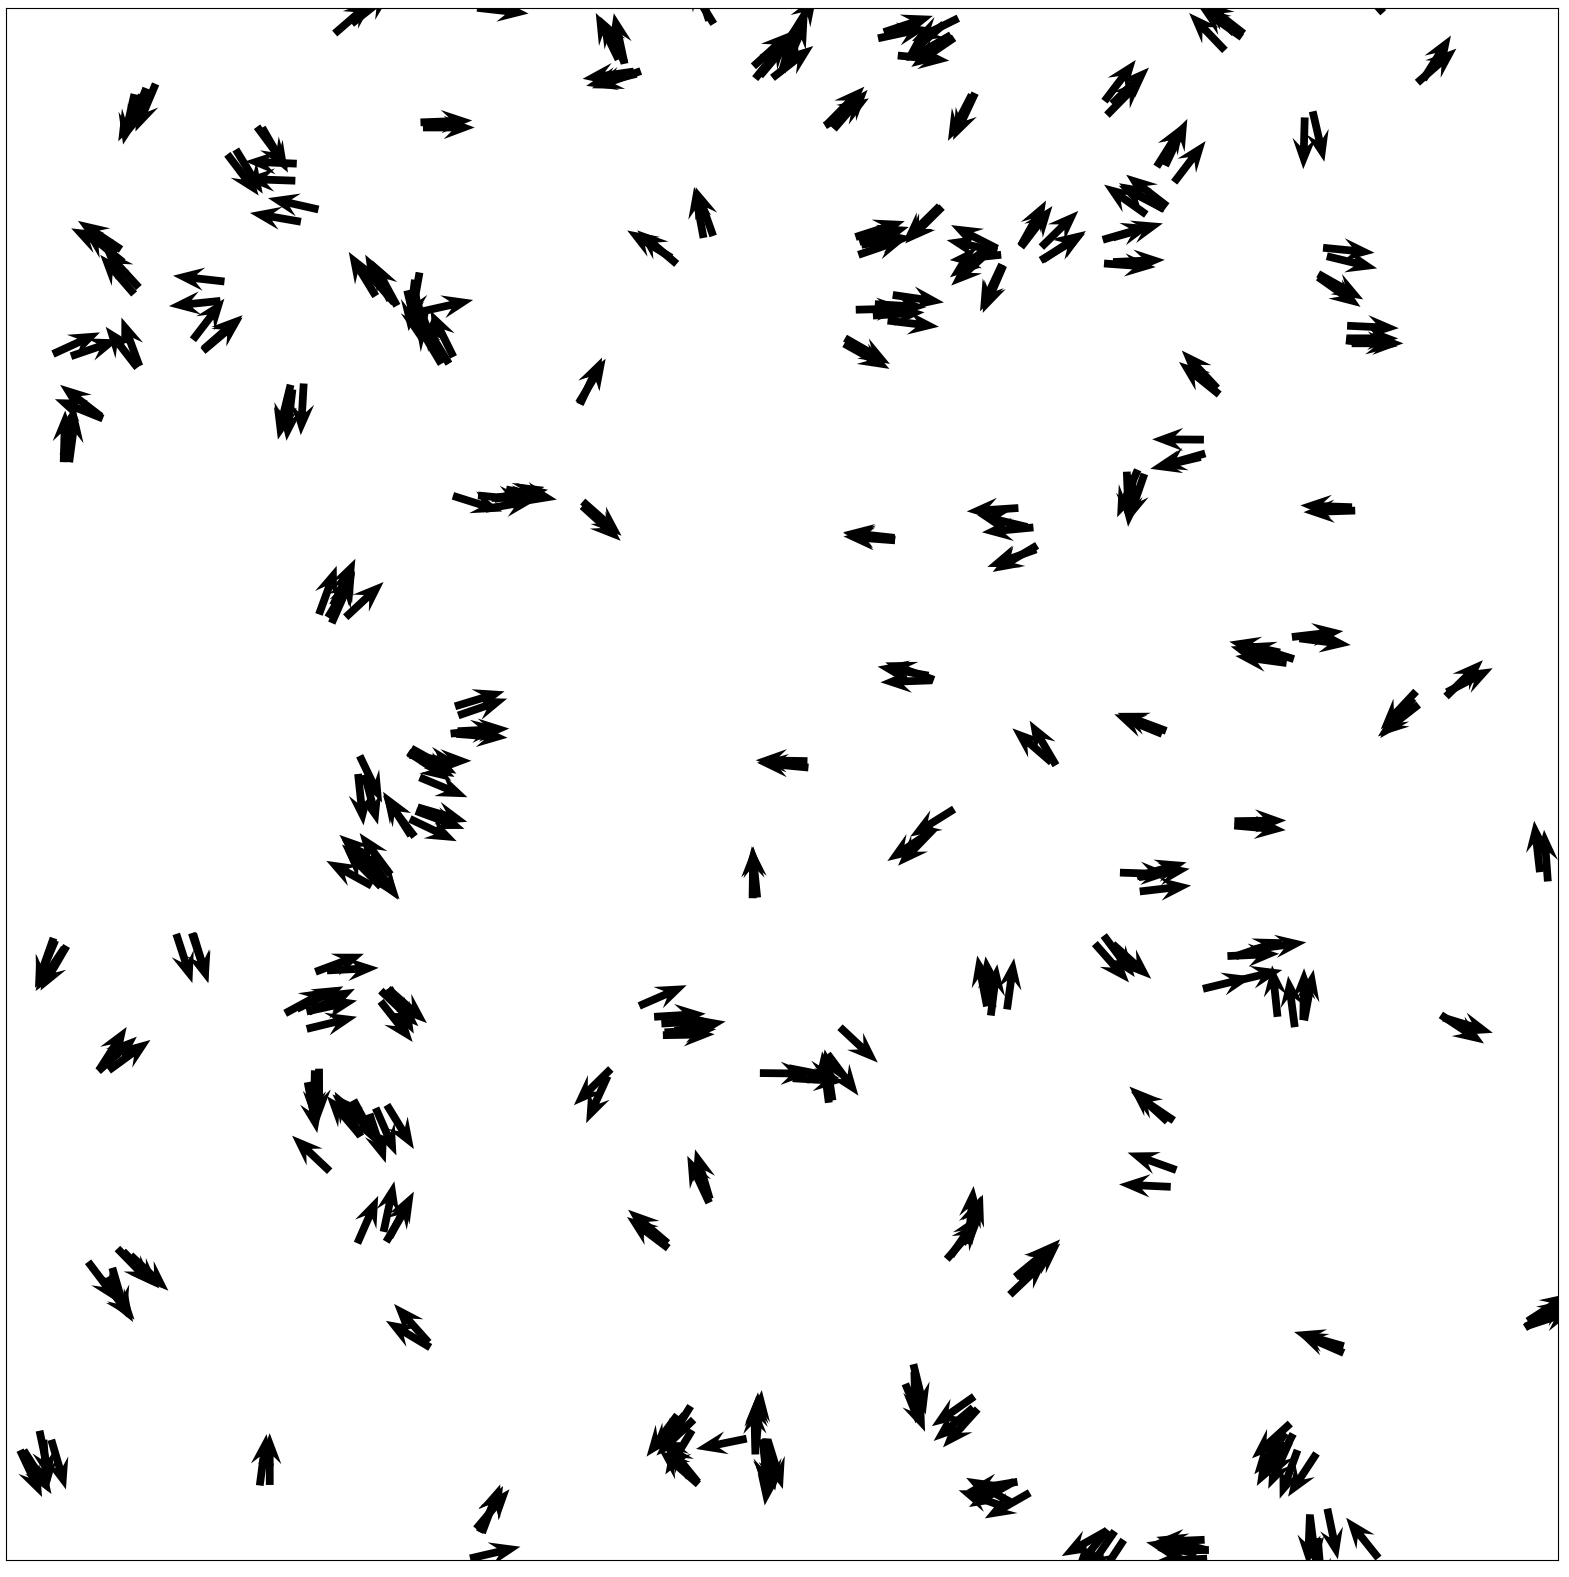
\includegraphics[width=0.3\textwidth]{plots/Snapshot_k1_n0.4.png}
    \label{fig:Snapshot_k1_n0.4}
  }
  \subfigure[$k=2$, $\eta=0.6$]{
    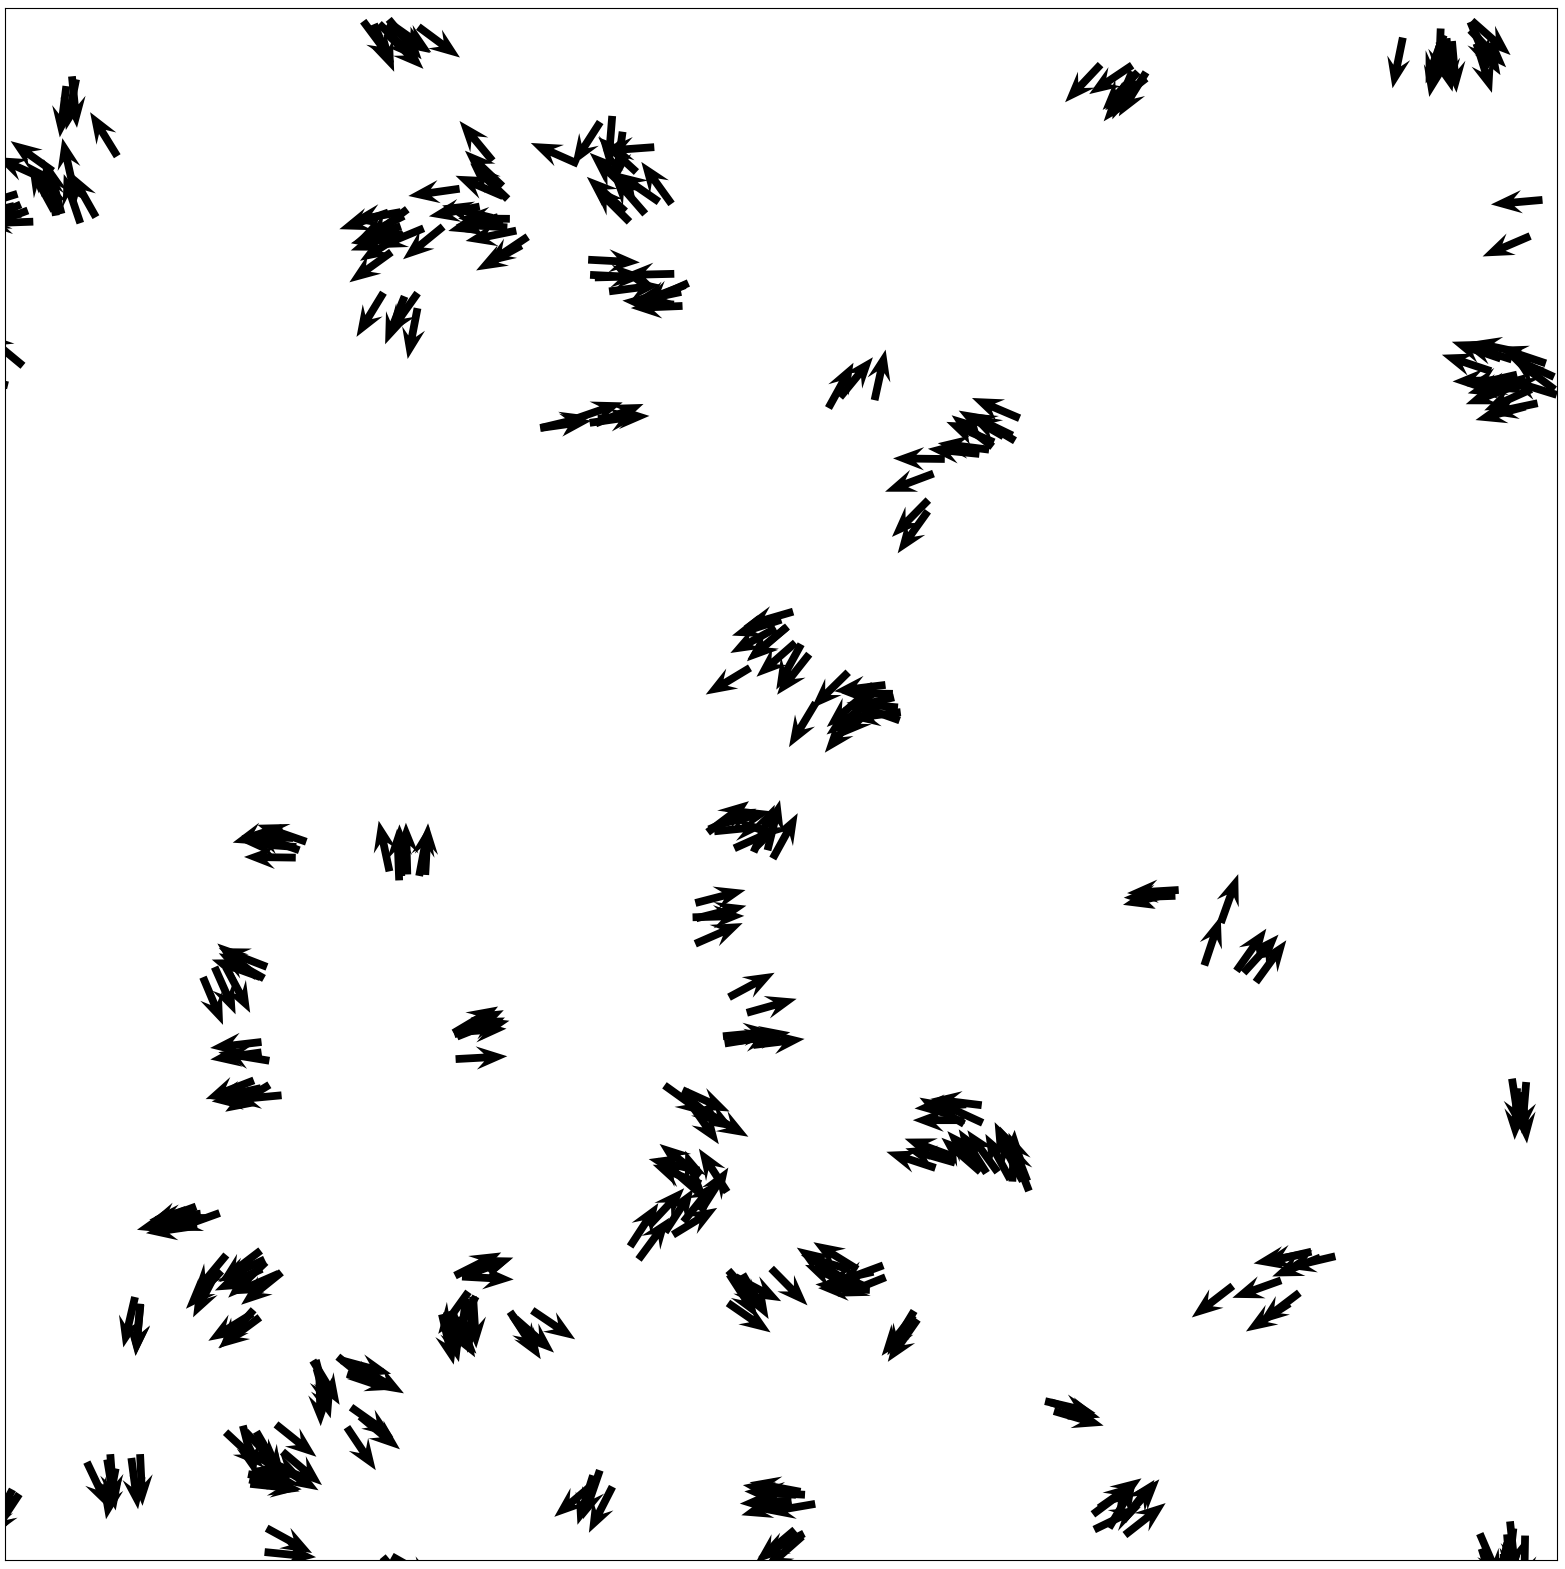
\includegraphics[width=0.3\textwidth]{plots/Snapshot_k2_n0.6.png}
    \label{fig:Snapshot_k2_n0.6}
  }
  \subfigure[$k=4$, $\eta=1.0$]{
    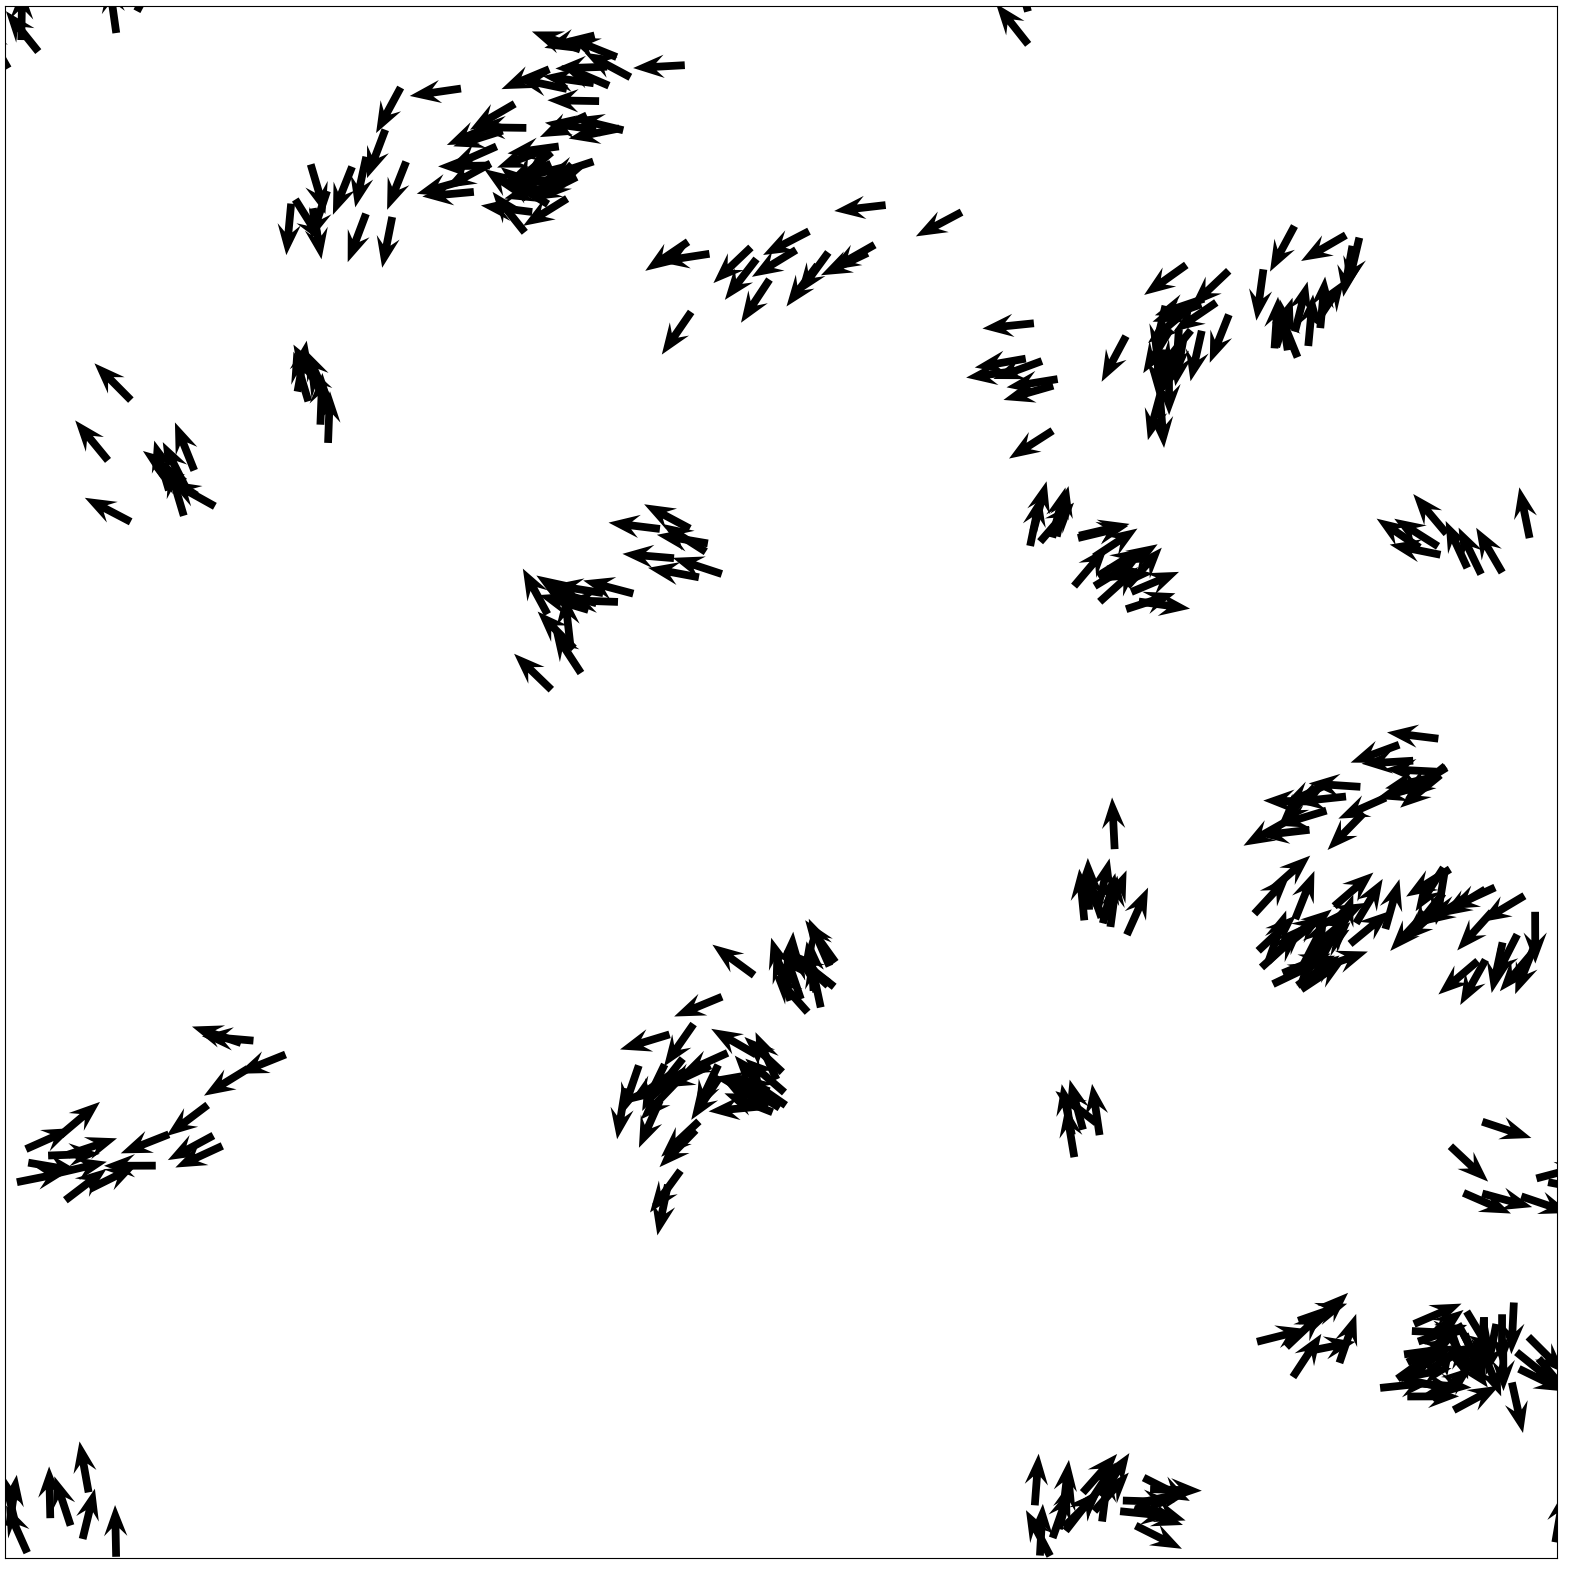
\includegraphics[width=0.3\textwidth]{plots/Snapshot_k4_n1.0.png}
    \label{fig:Snapshot_k4_n1.0}
  }
  \caption{Für geringes $k$ bilden sich kleine \textit{Schwarmpakete} aus, die nur sich selbst wahrnehmen können, sofern sie eine gewisse Distanz zu anderen Teilchen besitzen. Eine höhere Anzahl an topologischen Nachbarn vergrößert diese Pakete und weicht dieses Verhalten somit ein wenig auf. Wird das Rauschen $\eta$ jedoch erhöht, brechen diese Pakete auf und es ergibt sich ein Zustand, der an die Koexistenz von flüssiger und gasförmiger Phase erinnert. Diese Koexistenz ist erkennbar an den Stetigkeitssprüngen der ersten Ableitung der Messkurven in Abbildungen \ref{fig:Topologisch_1a_Referenz} und \ref{fig:Topologisch_1a}. Alle Simulationen wurden für $N=400$ und $\rho=4$ durchgeführt; Simulationsschritte ($\Tilde{t} < \num{150}$).}
  \label{fig:Snapshot_k_n}
\end{figure}

\newpage

\begin{figure}[h!]
    \centering
    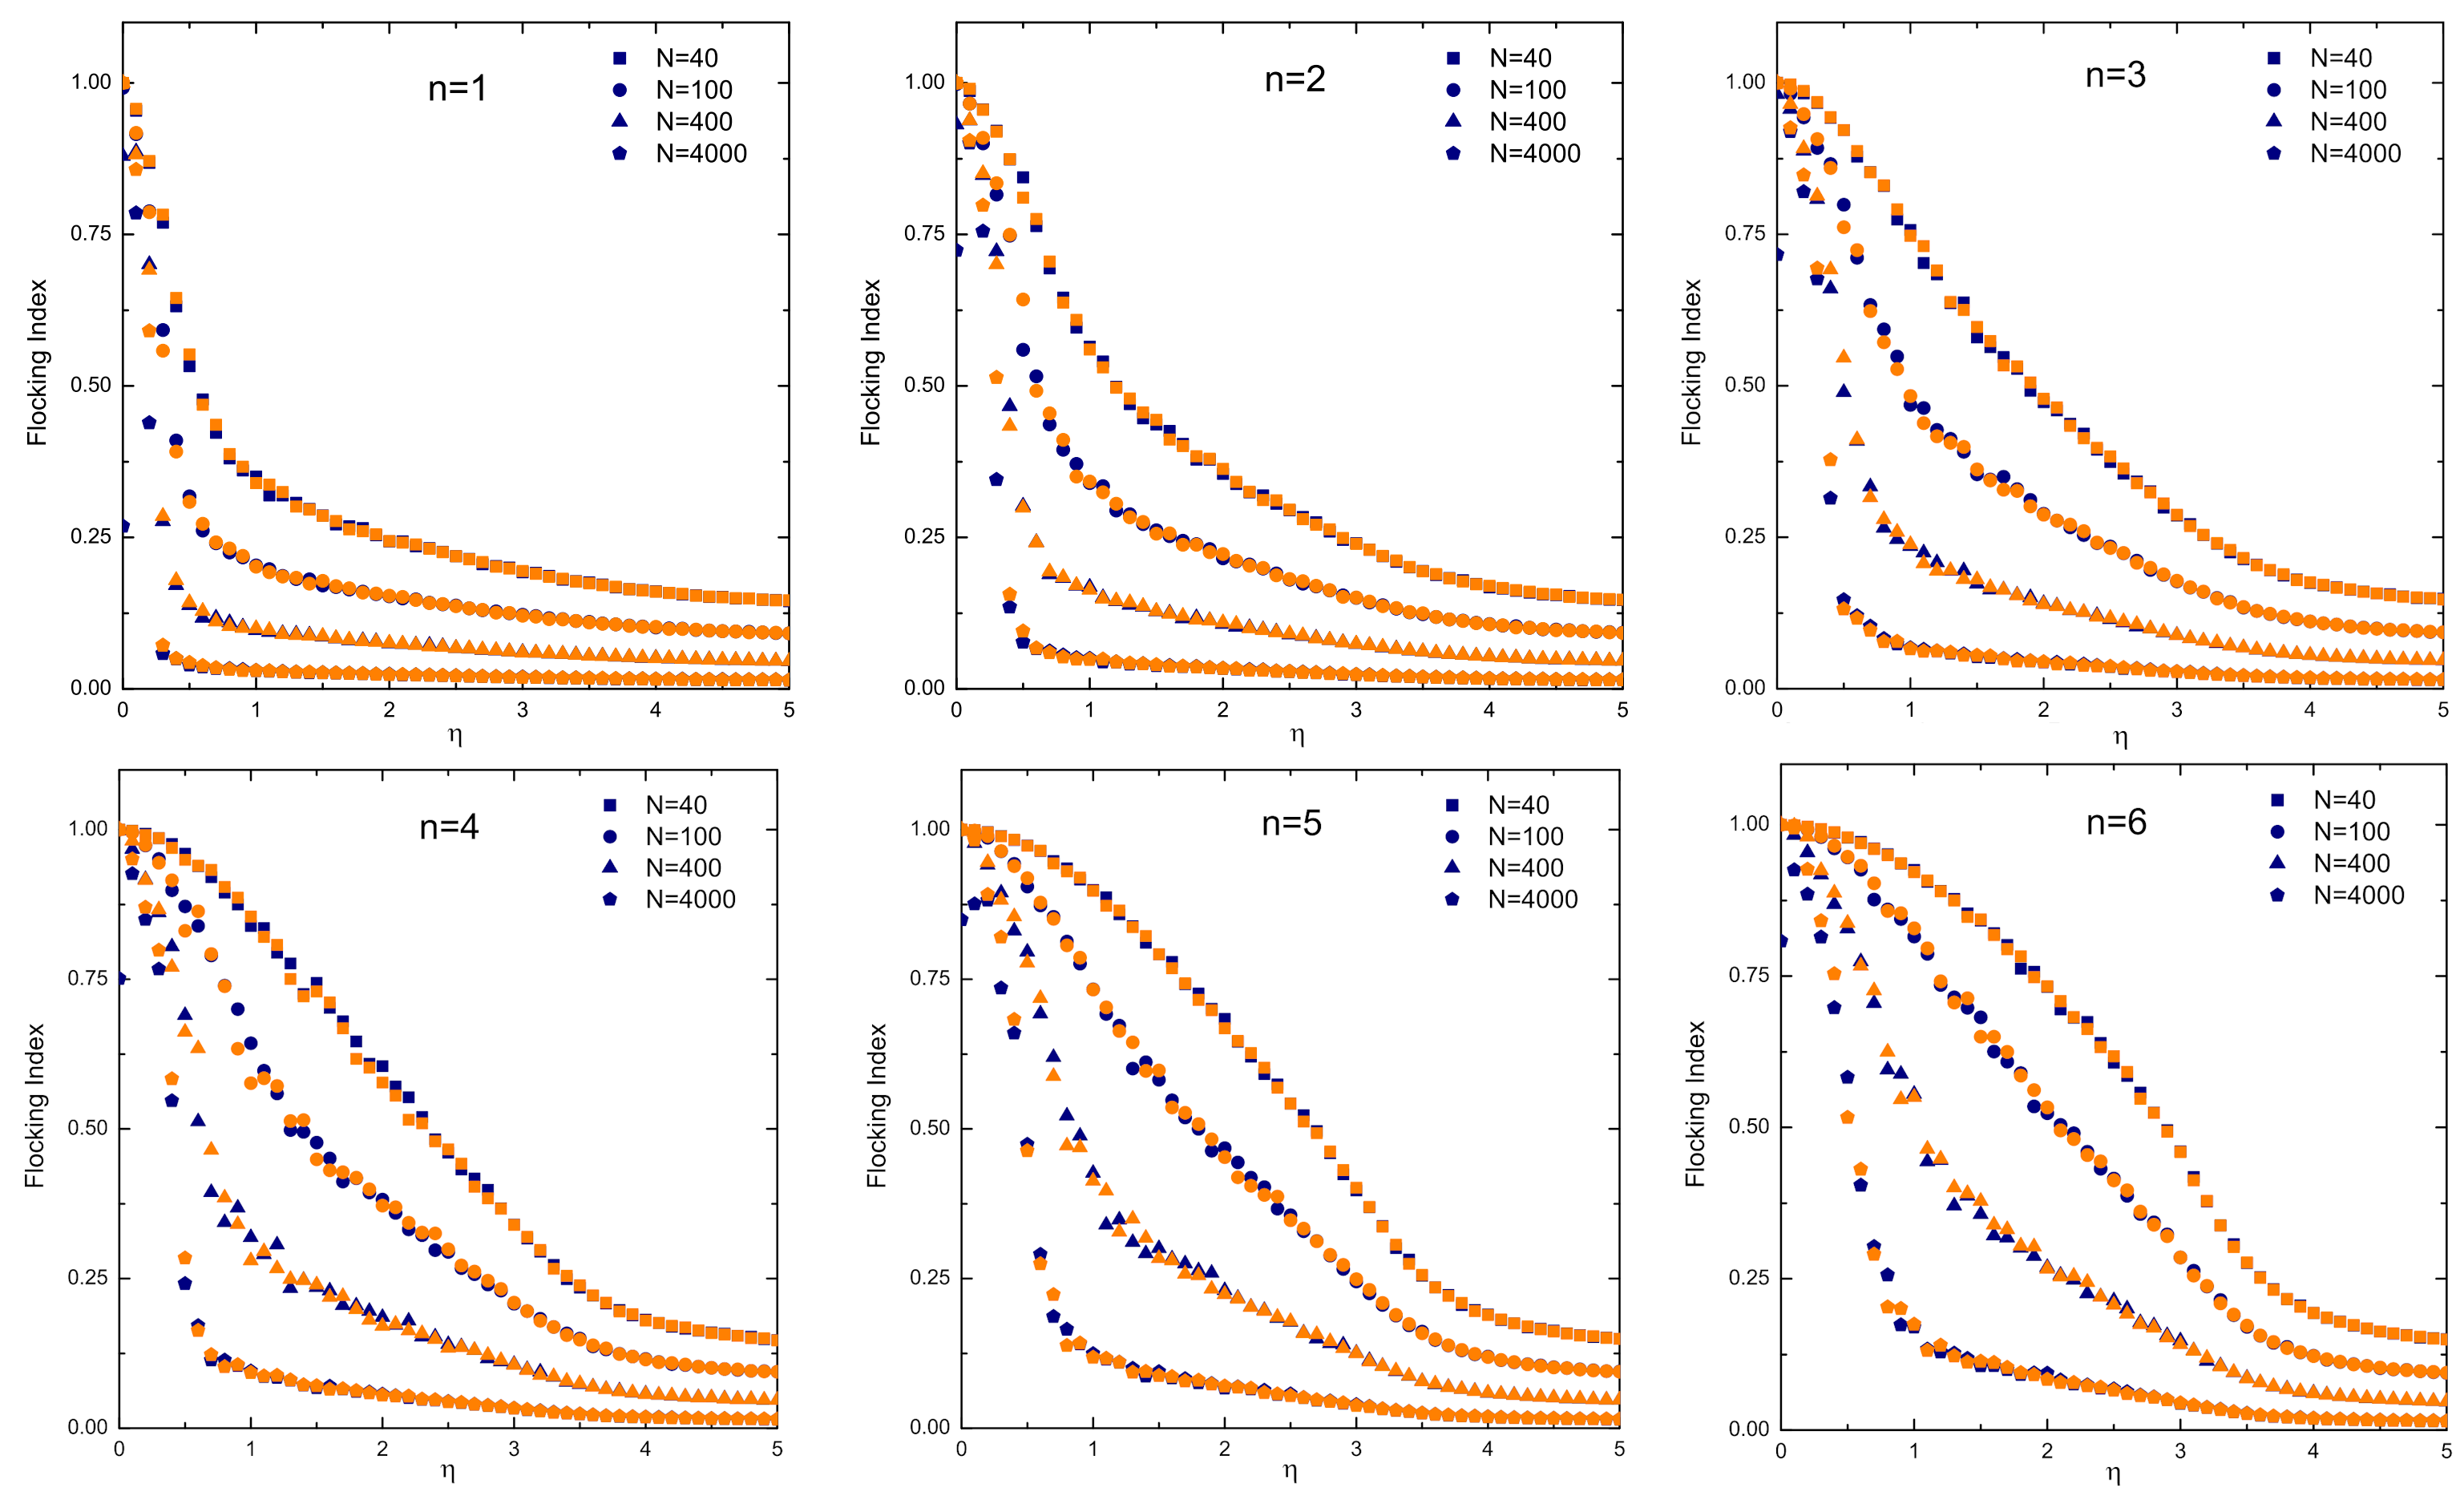
\includegraphics[width=.8\textwidth]{plots/Vicsek_1a_kNachbarn_Referenz.png}
    \caption{Simulationsergebnisse einer vorangegangenden Forschungsarbeit für das topologische Modell (hier n-Nachbarn, konstante Dichte $\rho = 4$). Die Ergebnisse dienen dem Vergleich mit Abbildung \ref{fig:Topologisch_1a} und stammen aus \cite{PhaseTransitions2013}.}
    \label{fig:Topologisch_1a_Referenz}
\end{figure}

\begin{figure}[h!]
    \centering
    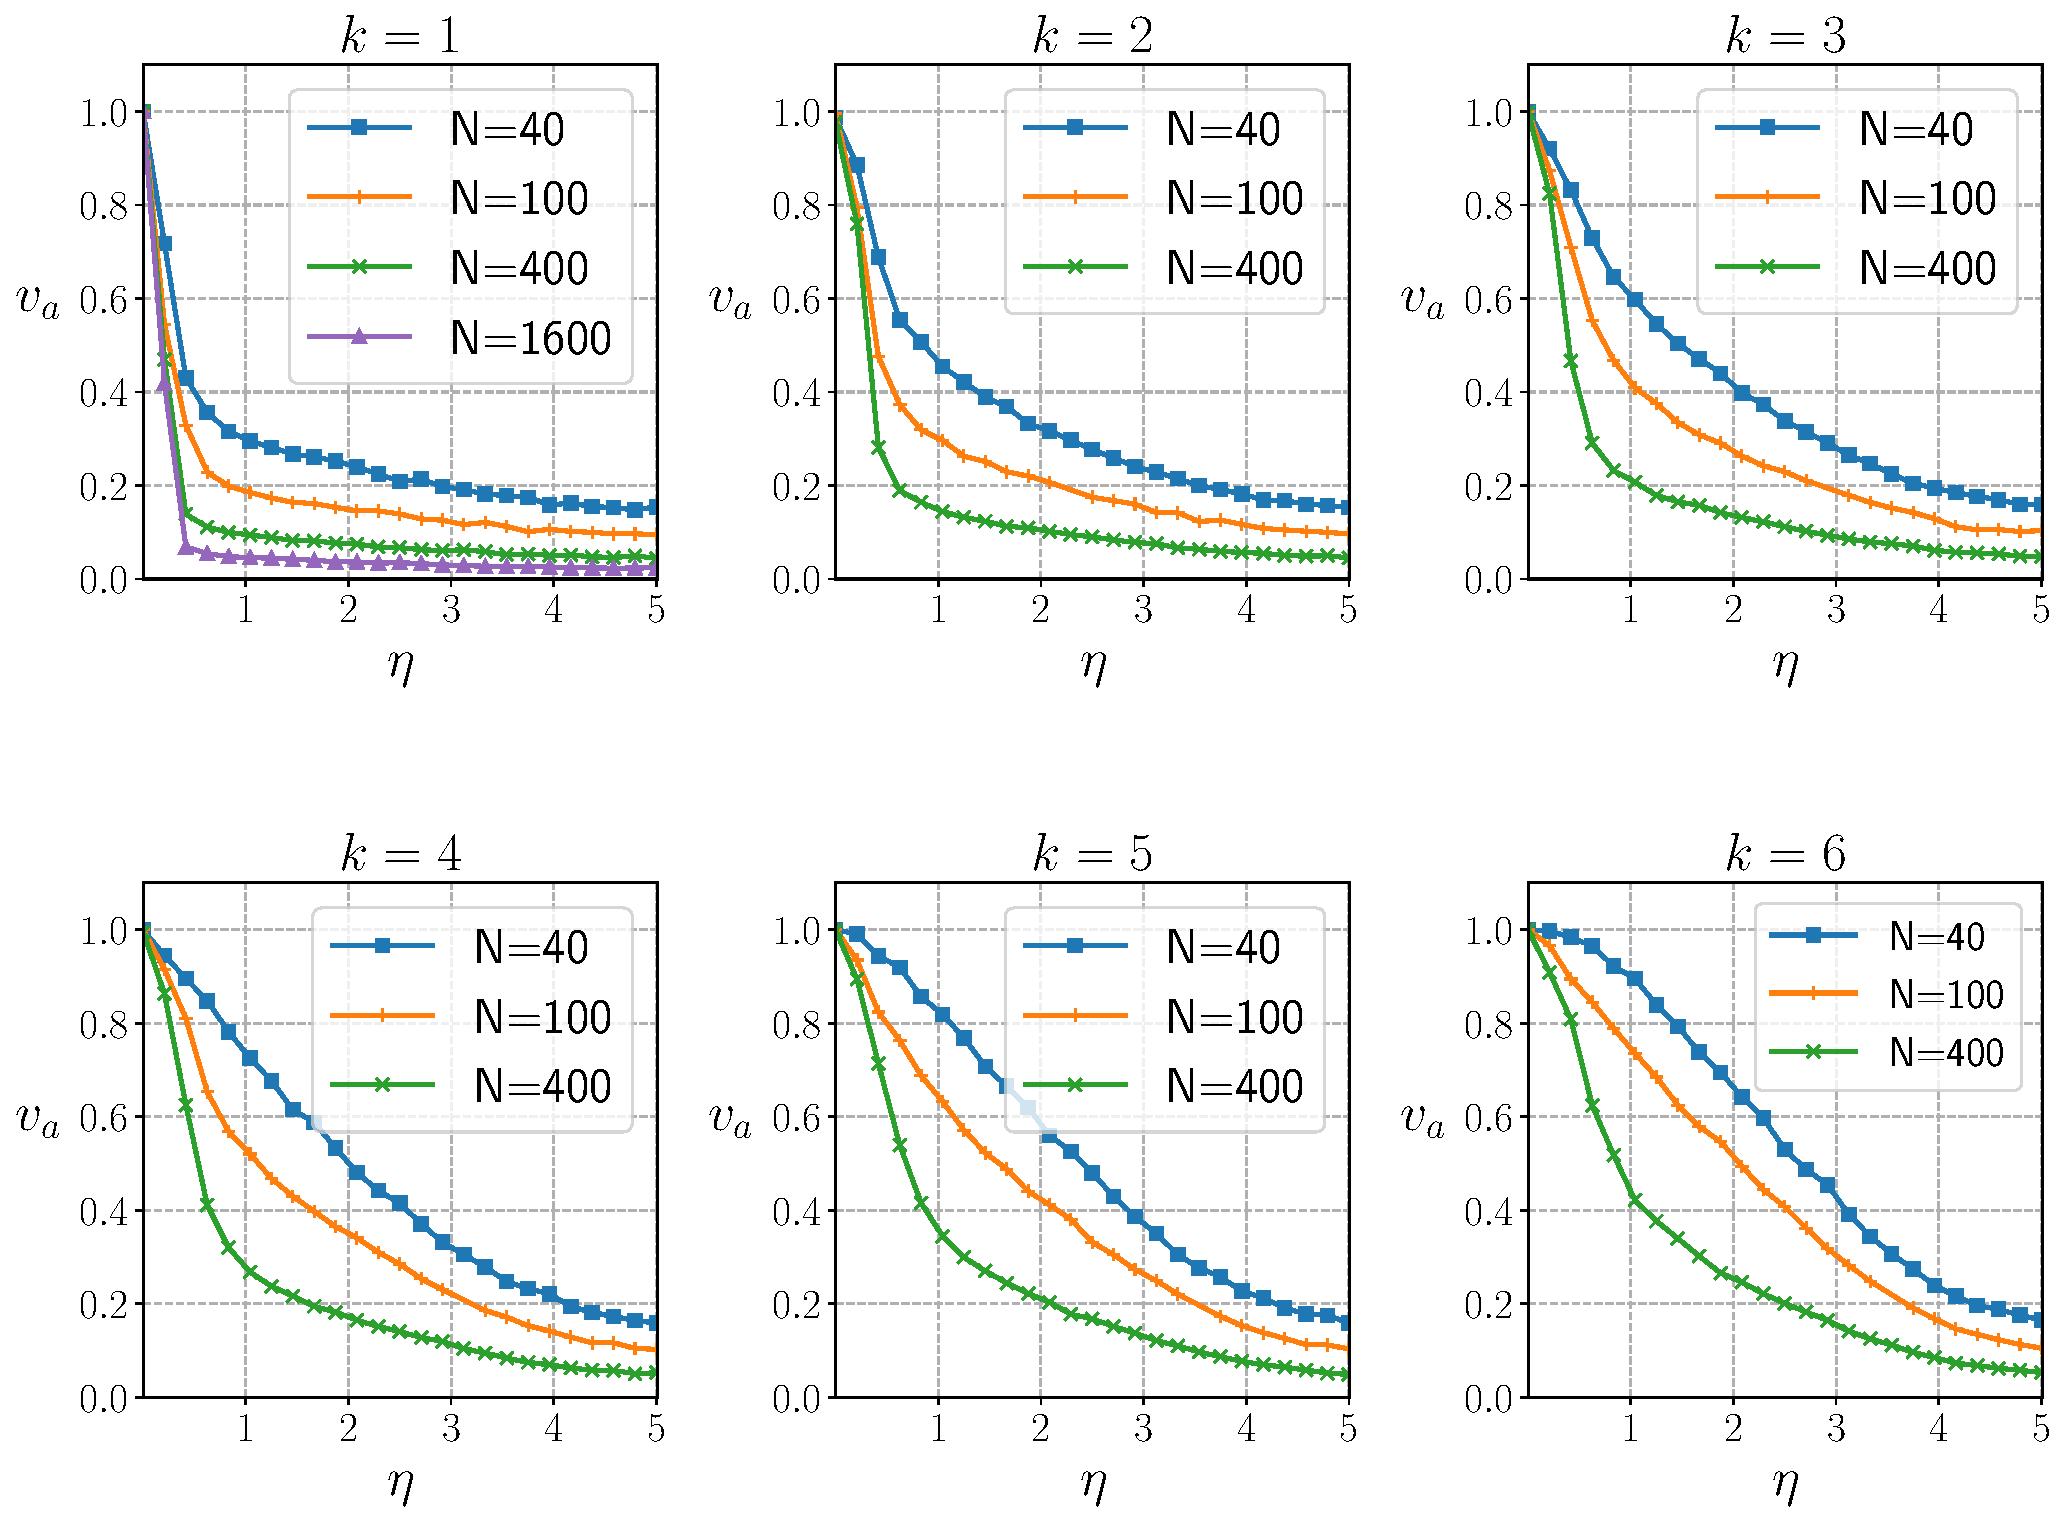
\includegraphics[width=.8\textwidth]{plots/Vicsek_1a_kNeighbors_final.pdf}
    \caption{Topologisches Modell mit konstanter Dichte $\rho = 4$. Die Daten stimmen gut mit den Ergebnissen aus \cite{PhaseTransitions2013} überein. Bei kleineren Teilchenzahlen von $N=\num{40}$ sind geringe Abweichungen erkennbar, während die restlichen Messungen weitgehend übereinstimmen.}
    \label{fig:Topologisch_1a}
\end{figure}

\newpage

\section{Metrisch-Topologischer Ansatz}

Die Hauptmotivation zur Verwendung eines topologischen Modells in dieser Arbeit ist die Fixierung der Nachbarteilchen-Anzahl. Im letzten Abschnitt wurde beobachtet, dass diese Modelle jedoch zu irregulären Schwarmpaket-Bildungen neigen, was das System instabil macht. Für einen qualitativen Vergleich der Modelle sind in Abbildung \ref{fig:Snapshot_r_n} drei Schnappschüsse des Vicsek-Modells dargestellt - mit gleichen Rausch-Einstellungen wie die zuvor gezeigten Schnappschüsse \ref{fig:Snapshot_k_n}.

\begin{figure}[ht]
  \centering
  \subfigure[$\eta=0.4$]{
    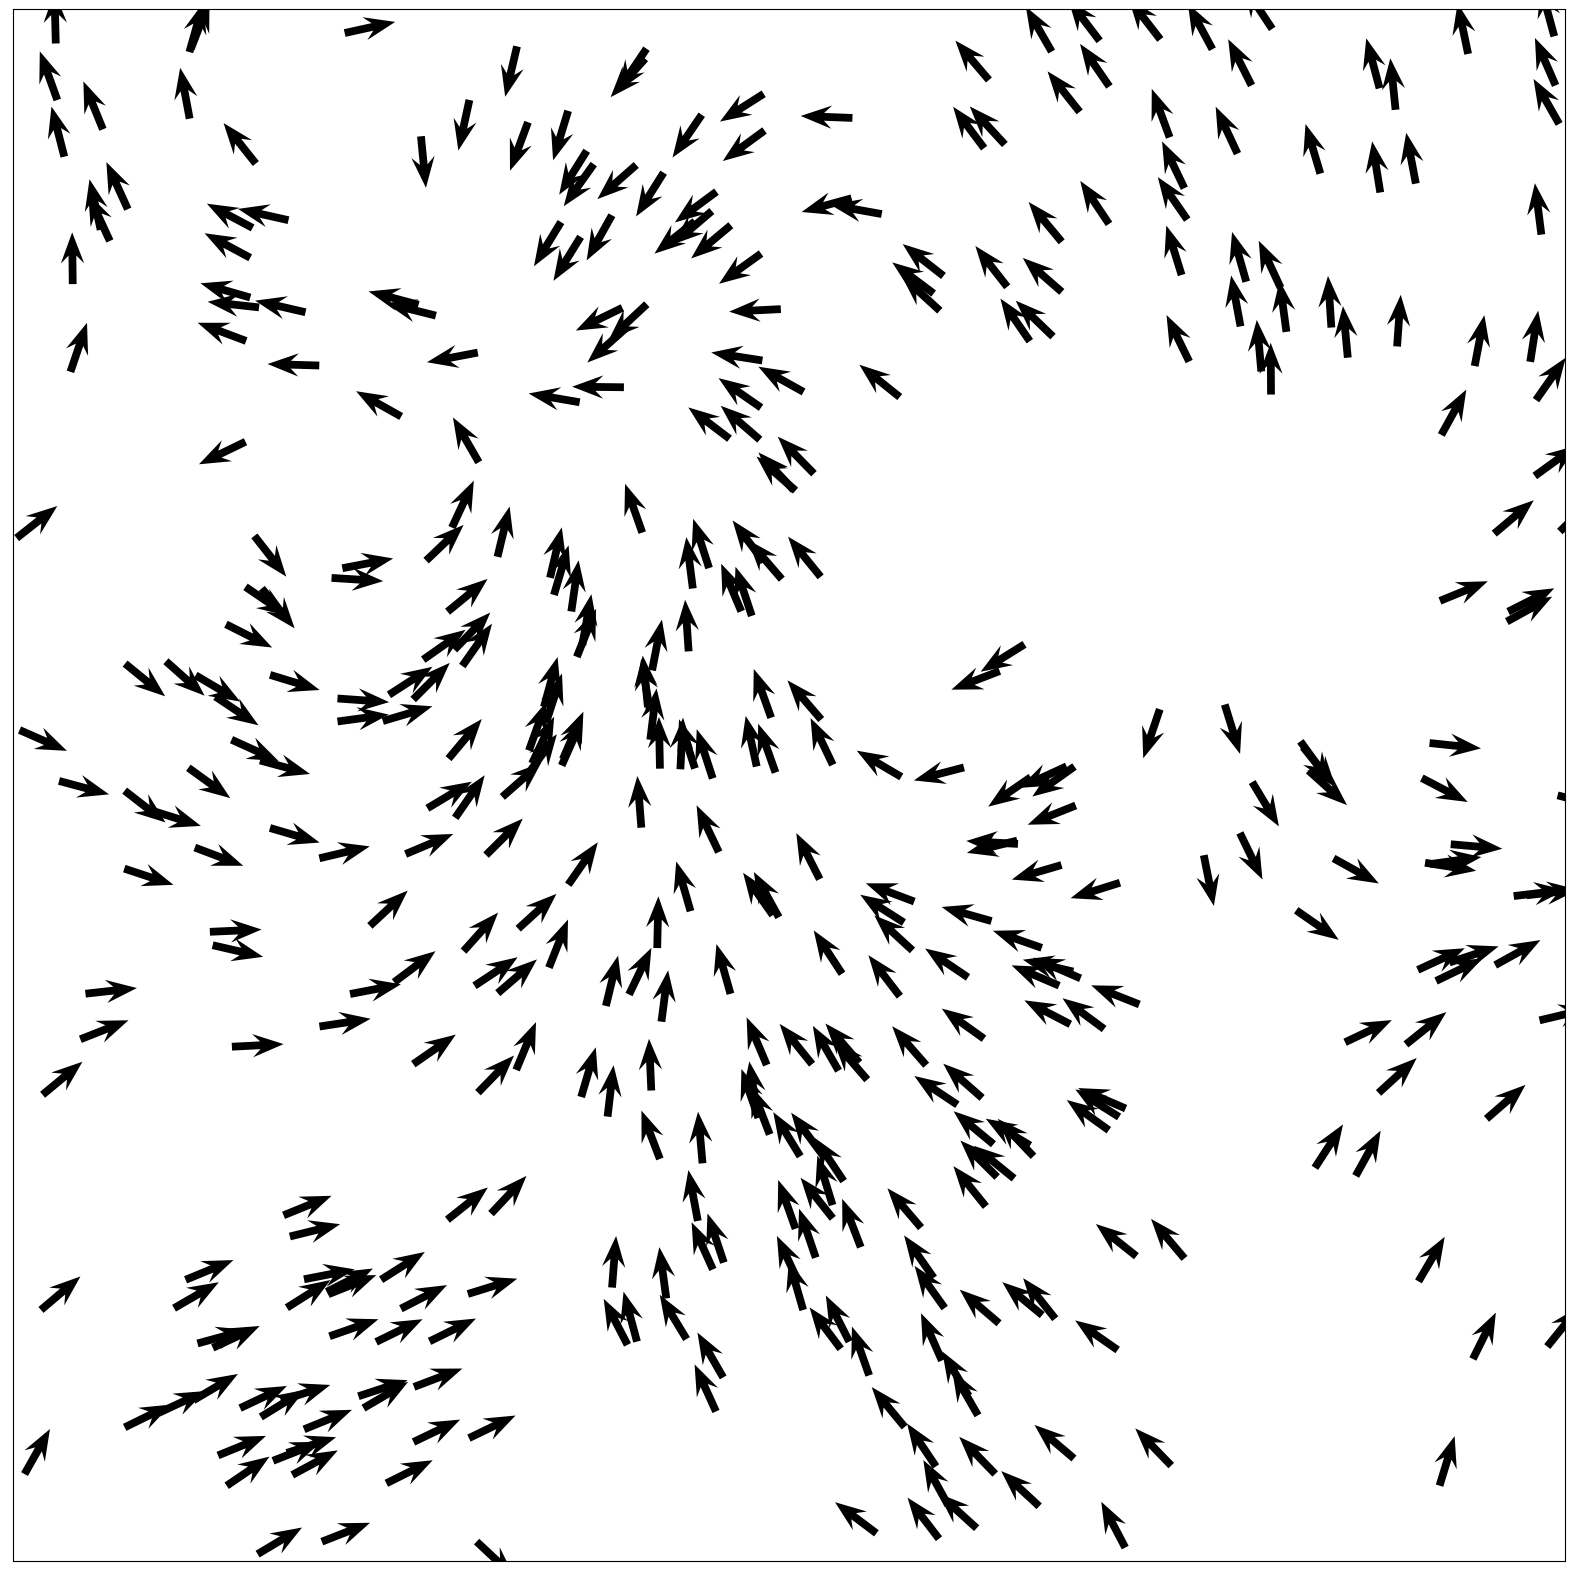
\includegraphics[width=0.3\textwidth]{plots/Snapshot_r1_n0.4.png}
    \label{fig:Snapshot_r1_n0.4}
  }
  \subfigure[$\eta=0.6$]{
    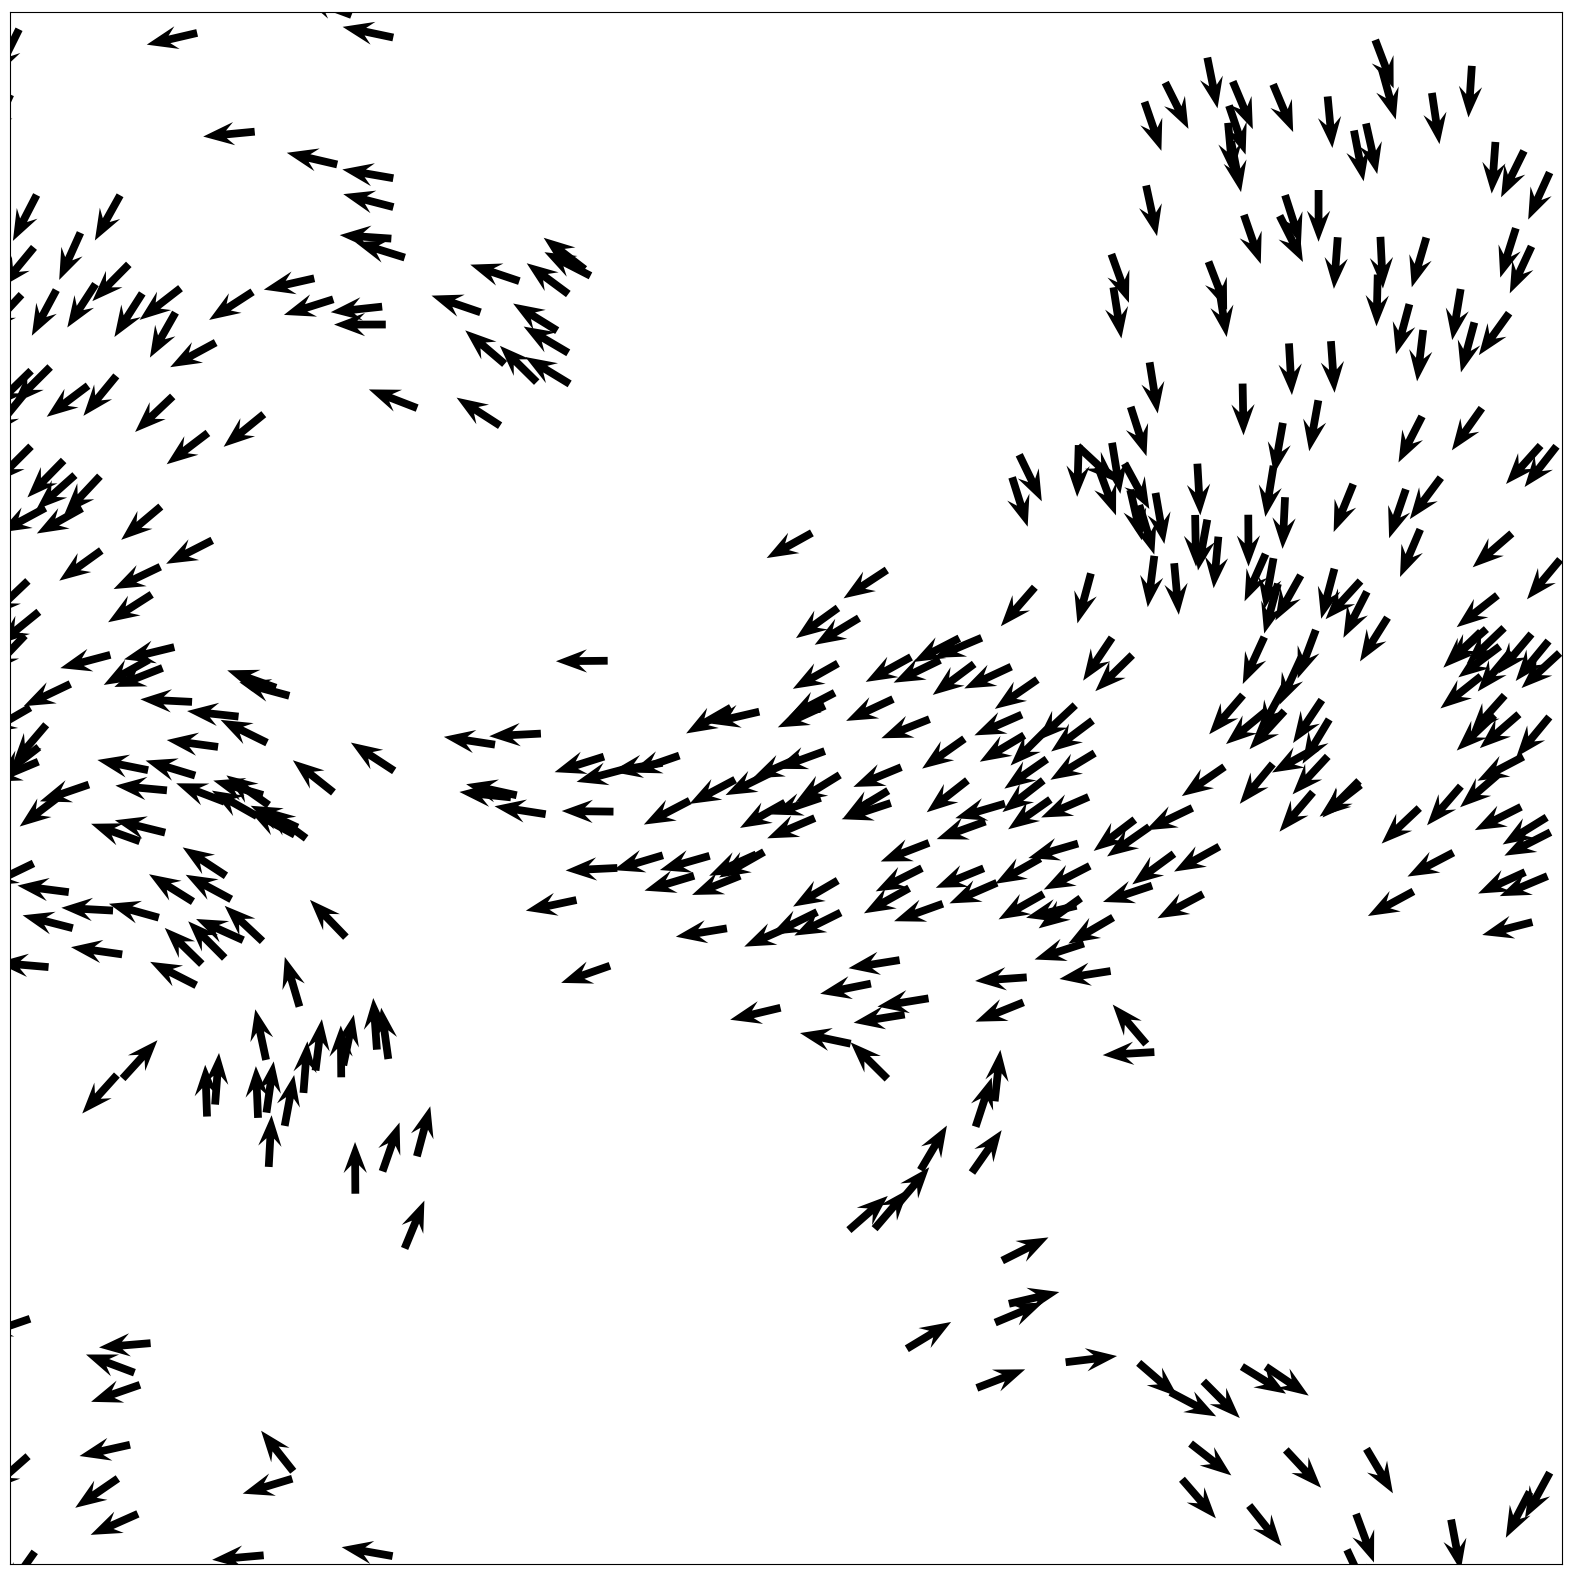
\includegraphics[width=0.3\textwidth]{plots/Snapshot_r1_n0.6.png}
    \label{fig:Snapshot_r1_n0.6}
  }
  \subfigure[$\eta=1.0$]{
    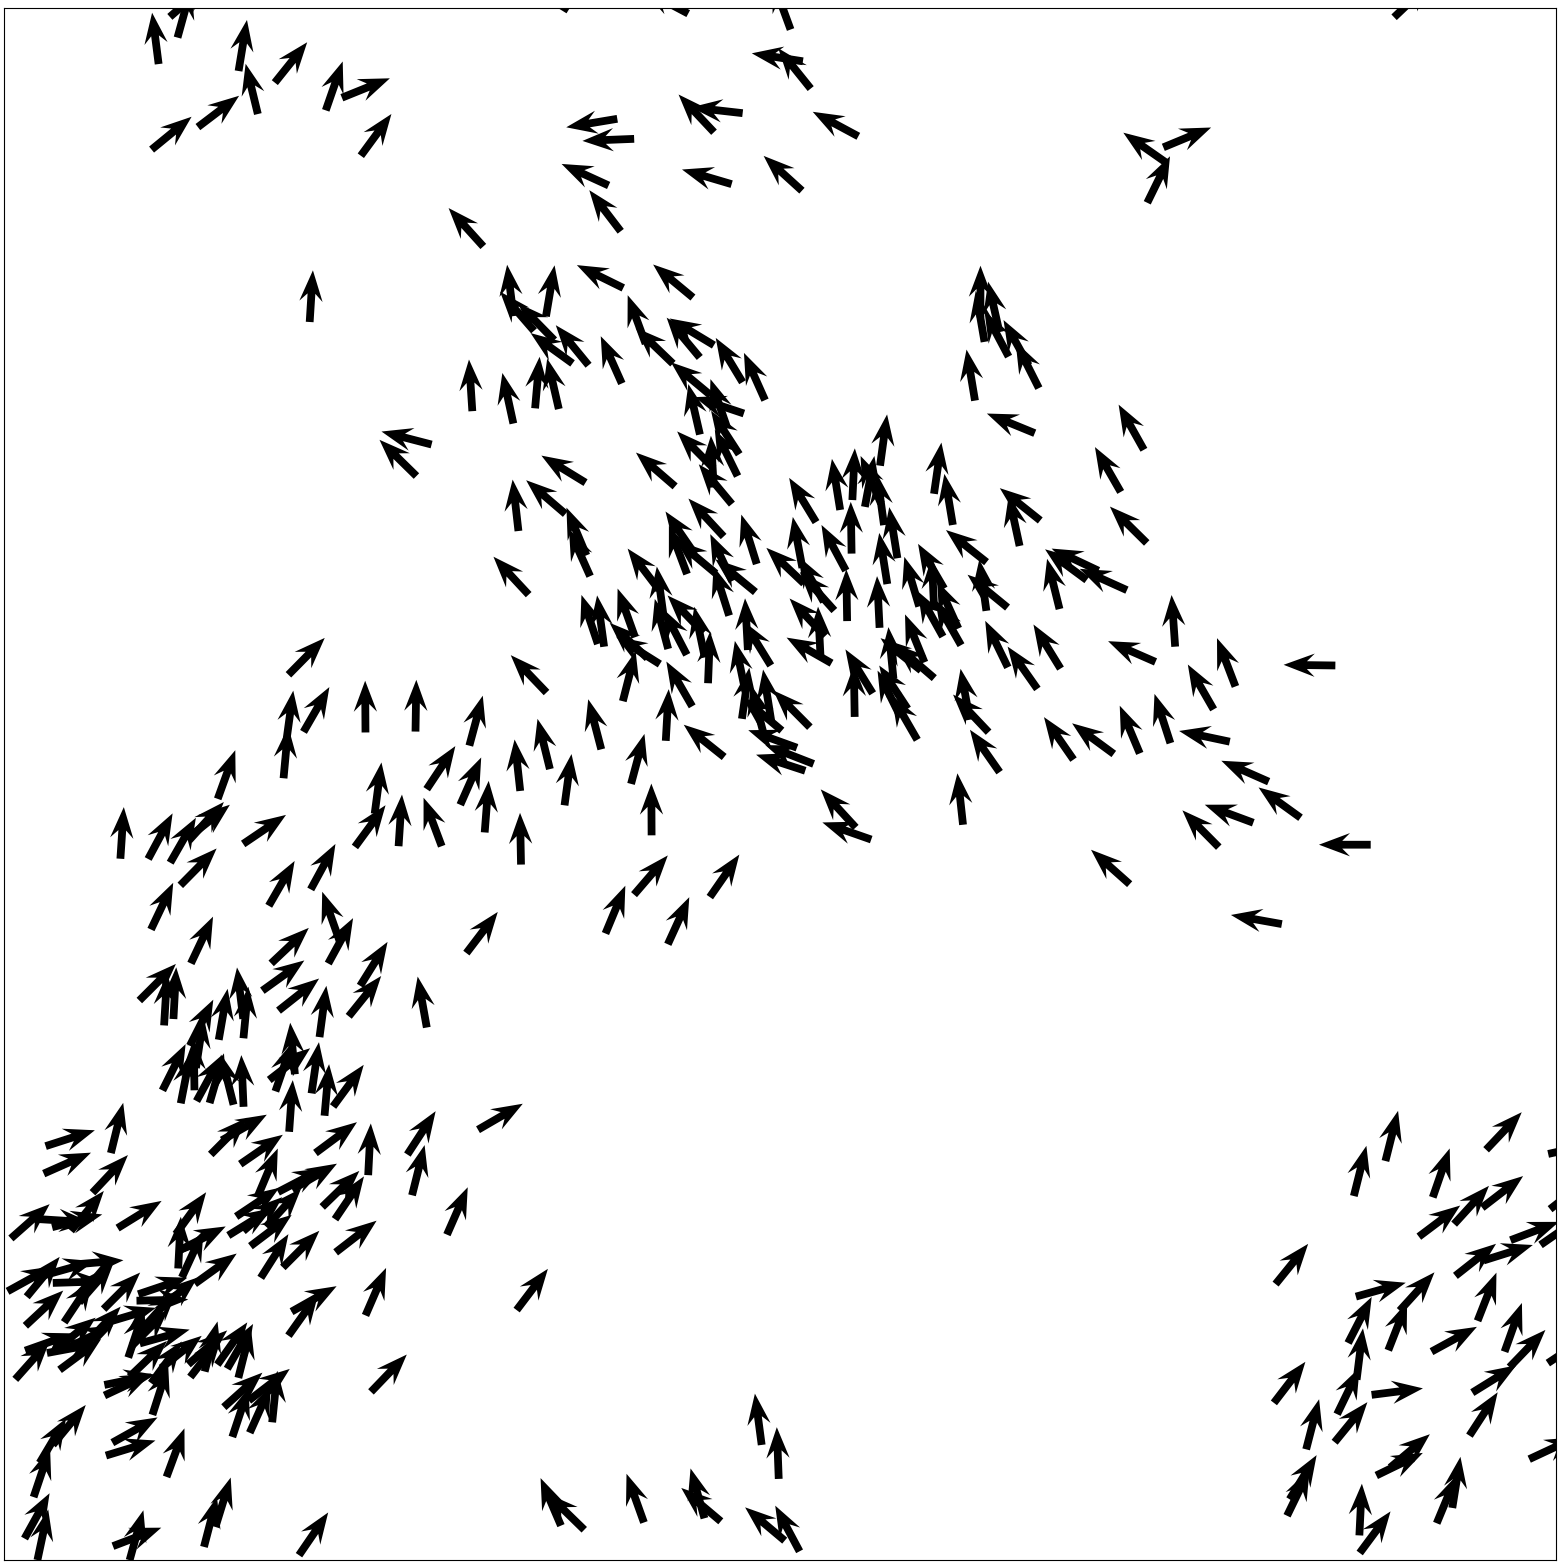
\includegraphics[width=0.3\textwidth]{plots/Snapshot_r1_n1.0.png}
    \label{fig:Snapshot_r1_n1.0}
  }
  \caption{Schnappschüsse des metrischen Vicsek-Modells für einen qualitativen Vergleich zu den anderen Modellen aus Abbildung \ref{fig:Snapshot_k_n} und \ref{fig:Snapshot_rk_n}. Es ist $N=400$ und $\rho=4$. Alle Schnappschüsse wurden nach nur sehr wenigen Simulationsschritten aufgenommen ($\Tilde{t} < \num{50}$).}
  \label{fig:Snapshot_r_n}
\end{figure}

\subsection{Einführung des neuen Modells}

Die Grundidee eines neuartigen Ansatzes besteht darin, den Wechselwirkungsradius $r$ eines metrischen Modells beizubehalten und damit ein wenig von der Stabilität solcher Modelle zurückzugewinnen. Eine mögliche Umsetzung dieser Idee ist also das Bestimmen von $k$ Nachbarn und dem Verwerfen aller Teilchen, die einen größeren Abstand als $r$ aufweisen. Diese Herangehensweise stellt jedoch eine \textit{Verschlechterung} der Stabilität dar, wie man sich schnell klarmachen kann: Die Instabilität topologischer Modelle resultiert aus der effektiven Kurzreichweitigkeit durch Stellen lokal hoher Dichte. Diese Kurzreichweitigkeit wird verstärkt, wenn nun auch noch Nachbarn ausgeschlossen werden, die weiter als $r$ entfernt sind.\\

Mit einer einzigen Modifikation kann dieses Modell jedoch signifikant verbessert werden (gemessen an der Stabilität und der Vergleichbarkeit mit dem Vicsek-Modell). Die Idee dieser Anpassung entsprang der Intuition: In Abbildung \ref{fig:RadialHistogram_plain} ist ein radiales Histogramm gezeigt, das die Perspektive eines einzelnen Teilchens zeigt. Dieses Teilchen sieht in seinem Wechselwirkungsradius exemplarisch zwei große Schwärme. In einem metrischen Modell würde es nun über alle Teilchen mitteln. Durch die topologische Einschränkung jedoch ist es auf $k$ Nachbarn beschränkt. Würde es sich hier um ein biologischen Fall handeln und die gezeigte Perspektive dem Sehen entsprechen, wäre es plausibel anzunehmen, dass das Auge in schnellen Situationen die Informationen der Umgebung abstrahiert und in gröbere \textit{Bereiche} einteilt. Falls nur $k$ Bereiche zur Verfügung stehen, müssen die Informationen in diesen Bereichen zusammengefasst werden. Dies entspräche einer Mittelung aller Teilchen in Bereichen gleicher Größe, wobei die \textit{Größe} hier der Teilchenanzahl entspricht. In einem Histogramm kann das mittels $k$-Quantile dargestellt werden. In der Abbildung sind beispielhaft $8$-Quantile gezeigt, die die Daten in gleich große Teilchenzahl-Bereiche teilen. Diese Bereiche können dann gemittelt werden, um die zuvor motivierte Überlegung umzusetzen.\\

In der Praxis ist diese Methodik aber umständlich und rechenintensiv. Ein wesentlich eleganterer Ansatz mit vergleichbarer Wirkung kann über einen stochastischen Zugang erreicht werden. Statt einer komplexen Bereichsaufteilung können zunächst alle Kandidaten im Wechselwirkungsradius $r$ bestimmt werden. Anschließend werden \textbf{zufällig} $k$ Nachbarn aus diesem Pool bestimmt. Mit einer zunehmenden Anzahl von Simulationsschritten entspricht dieser stochastische Ansatz mehr und mehr der Mittelung der $k$ Bereiche. Im gewissen Sinne wird dieses deterministisches Problem dadurch mit Monte-Carlo-Methoden gelöst.

\begin{figure}[h]
  \centering
  \subfigure[]{
    
\includegraphics[width=0.45\textwidth]{plots/RadialHistogram_plain.pdf}
    \label{fig:RadialHistogram_plain}
  }
  \subfigure[]{
    
\includegraphics[width=0.45\textwidth]{plots/RadialHistogram_quantile.pdf}
    \label{fig:RadialHistogram_quantile}
  }
  \caption{Beispielhafte Darstellung von zwei Schwärmen unterschiedlicher Größe und Ausrichtung. Die Histogramme beschreiben die Sichtweise eines einzelnen Teilchens, das diese beiden Schwärme gleichzeitig sieht (Imitation des Vicsek-Modell-Wechselwirkungsradius). \textbf{Links:} Radiales, uninterpretiertes Histogramm aus Sicht eines Teilchens. \textbf{Rechts:} Unterteilung des Histogramms in $k$-Quantile mit $k=8$. Es wird dasselbe System wie in \ref{fig:RadialHistogram_plain} betrachtet.}
  \label{fig:RadialHistograms}
\end{figure}

\begin{figure}[h!]
    \centering
    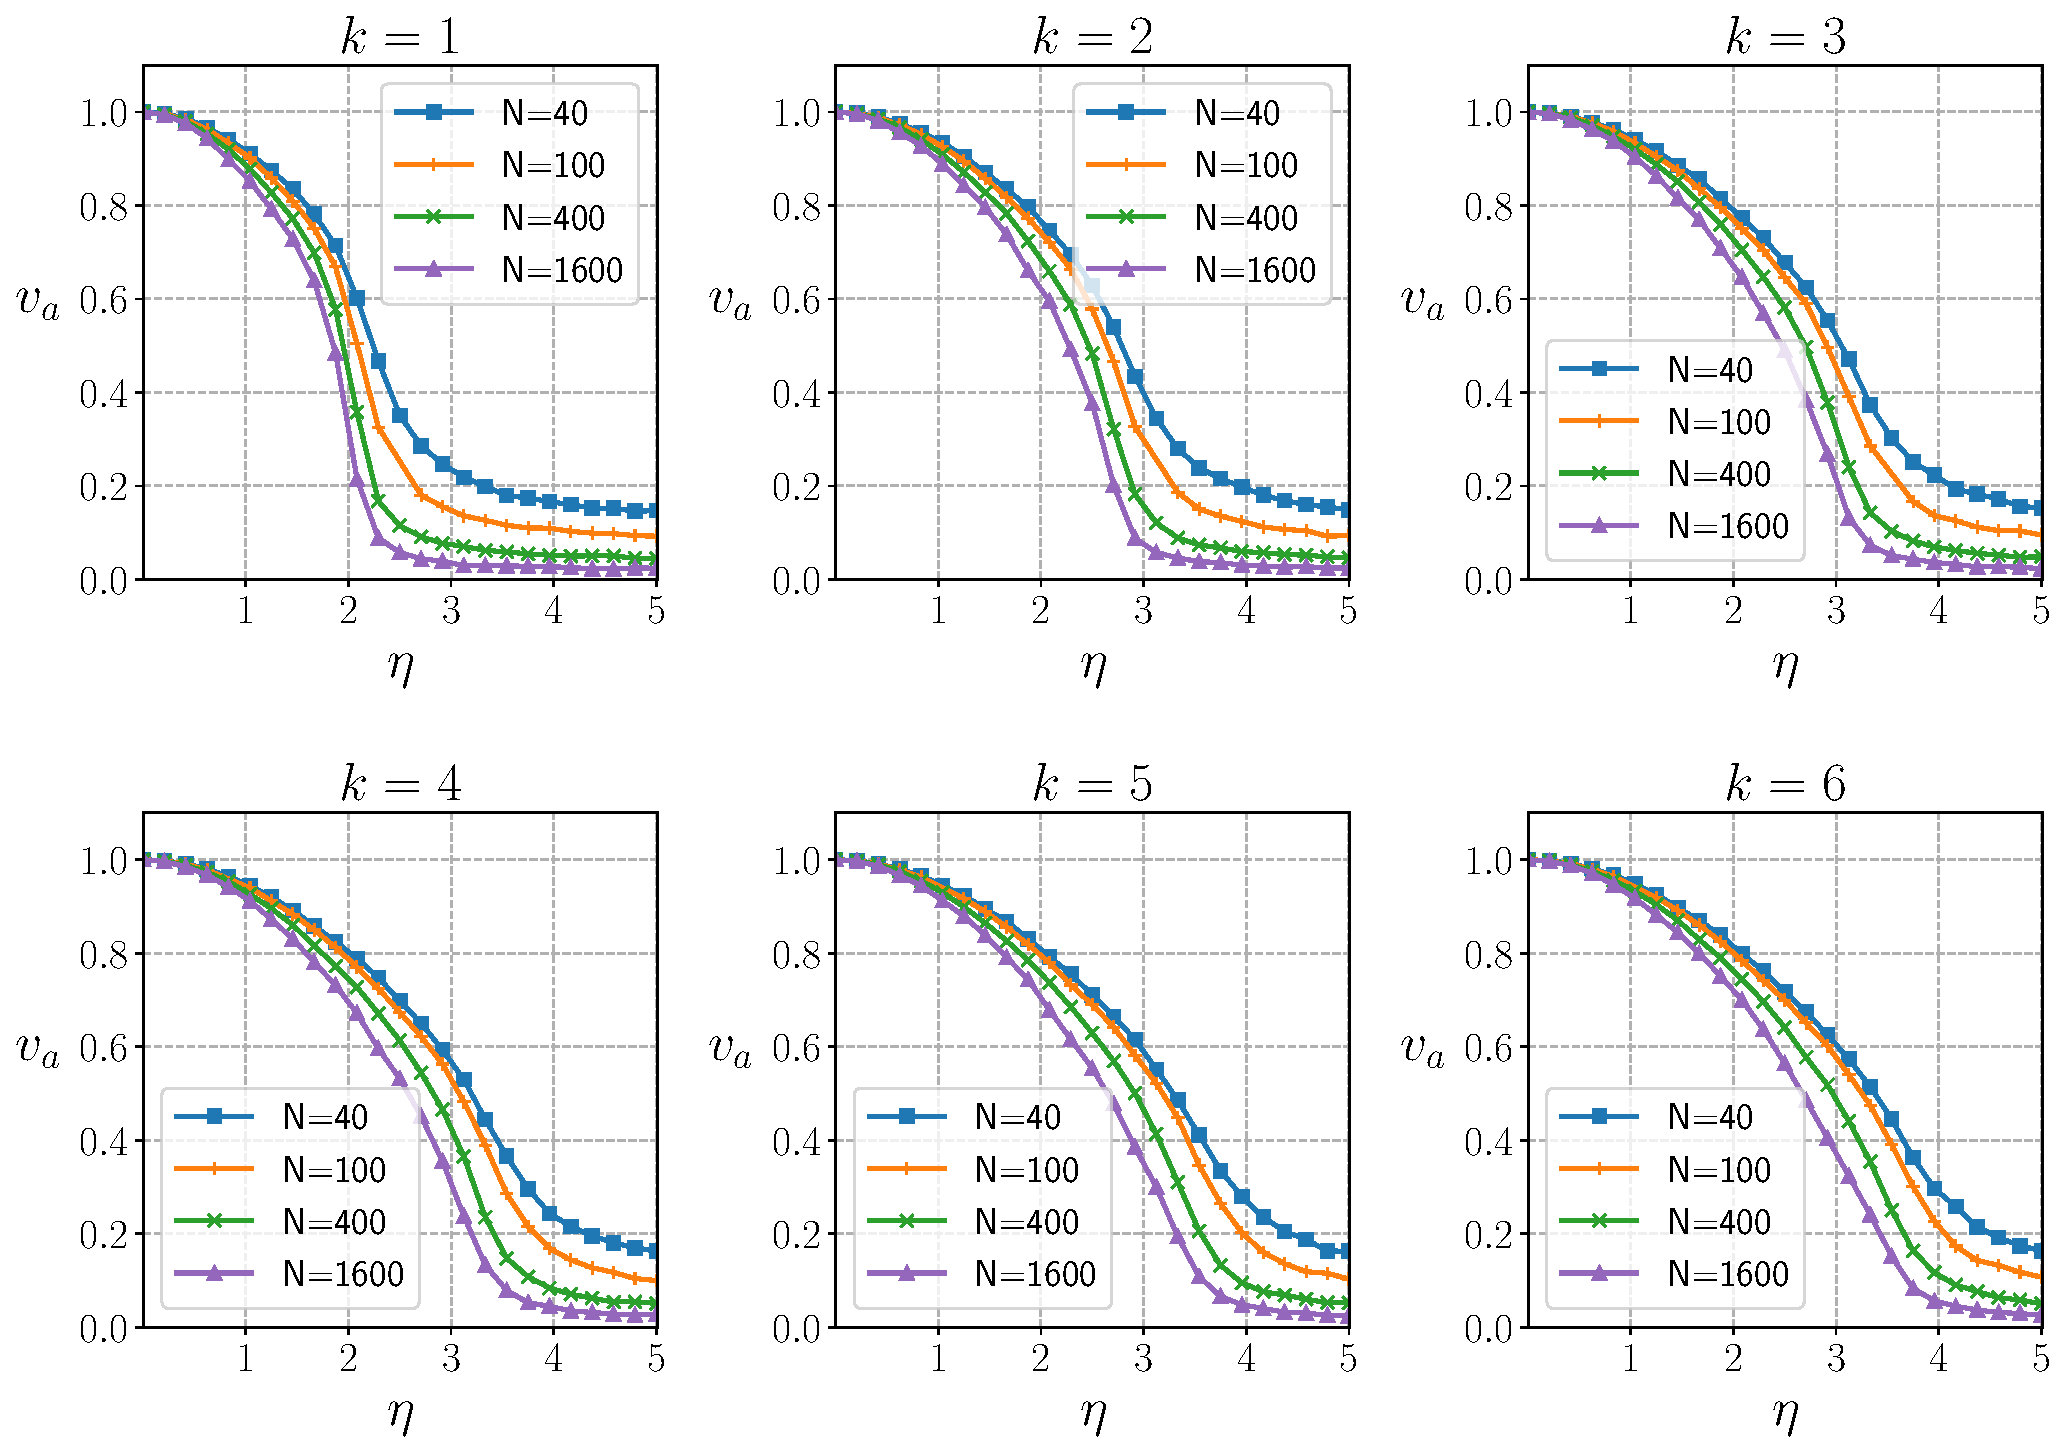
\includegraphics[width=.9\textwidth]{plots/Vicsek_1a_rkFixedRadius_final.pdf}
    \caption{Metrisch-Topologisches Modell mit konstanter Dichte $\rho = 4$.}
    \label{fig:MetrischTopologisch_1a}
\end{figure}

\newpage

\subsection{Messergebnisse}

In Abbildung \ref{fig:MetrischTopologisch_1a} sind die Messergebnisse des metrisch-topologischen Modells zu sehen. Für die Nachbarschafts-Bestimmung wurde die zuvor diskutierte stochastische Modifikation angewendet, was den Verlauf der Messkurven im Vergleich zu dem rein topologischen Modell deutlich ändert. Insbesondere für eine geringe Anzahl an Nachbarn verhält sich das Modell bei geringem Rauschen wesentlich stabiler. Die \textit{Knicke} bzw. Unstetigkeiten in den ersten Ableitungen sind verschoben, wenn nicht sogar aufgehoben.\\

Ein Blick auf die Schnappschüsse \ref{fig:Snapshot_rk_n} verdeutlicht den großen Unterschied zu dem rein topologischen Modell und die Ähnlichkeit zu dem Vicsek-Modell. Obwohl pro Simulationsschritt nur $k$ Nachbarn ausgewählt werden, ist keine Paket-Bildung kleinerer Schwärme mehr beobachtbar und die Form ähnelt den strom-artigen Strukturen eines metrischen Modells. Ein Unterschied zu dem Vicsek-Modell ist insofern erkennbar, als dass die Schwärme des neuartigen Modells keine scharfen Kurven aufweisen (siehe zum Vergleich die ausgeprägteren \textit{Wirbel} in Abbildung \ref{fig:Snapshot_r1_n0.4}). Dies ist auch plausibel, da in den Situationen, in denen viele Teilchen aus verschiedensten Richtungen aufeinandertreffen, das metrisch-topologischen Modell nicht alle Nachbarn in einem Zeitschritt gleichzeitig berücksichtigen kann. Daher sind die Schwärme für kleinere $k$ im Vergleich zum metrischen Modell strukturell geglättet.\\

\begin{figure}[h!]
  \centering
  \subfigure[$k=1$, $\eta=0.4$]{
    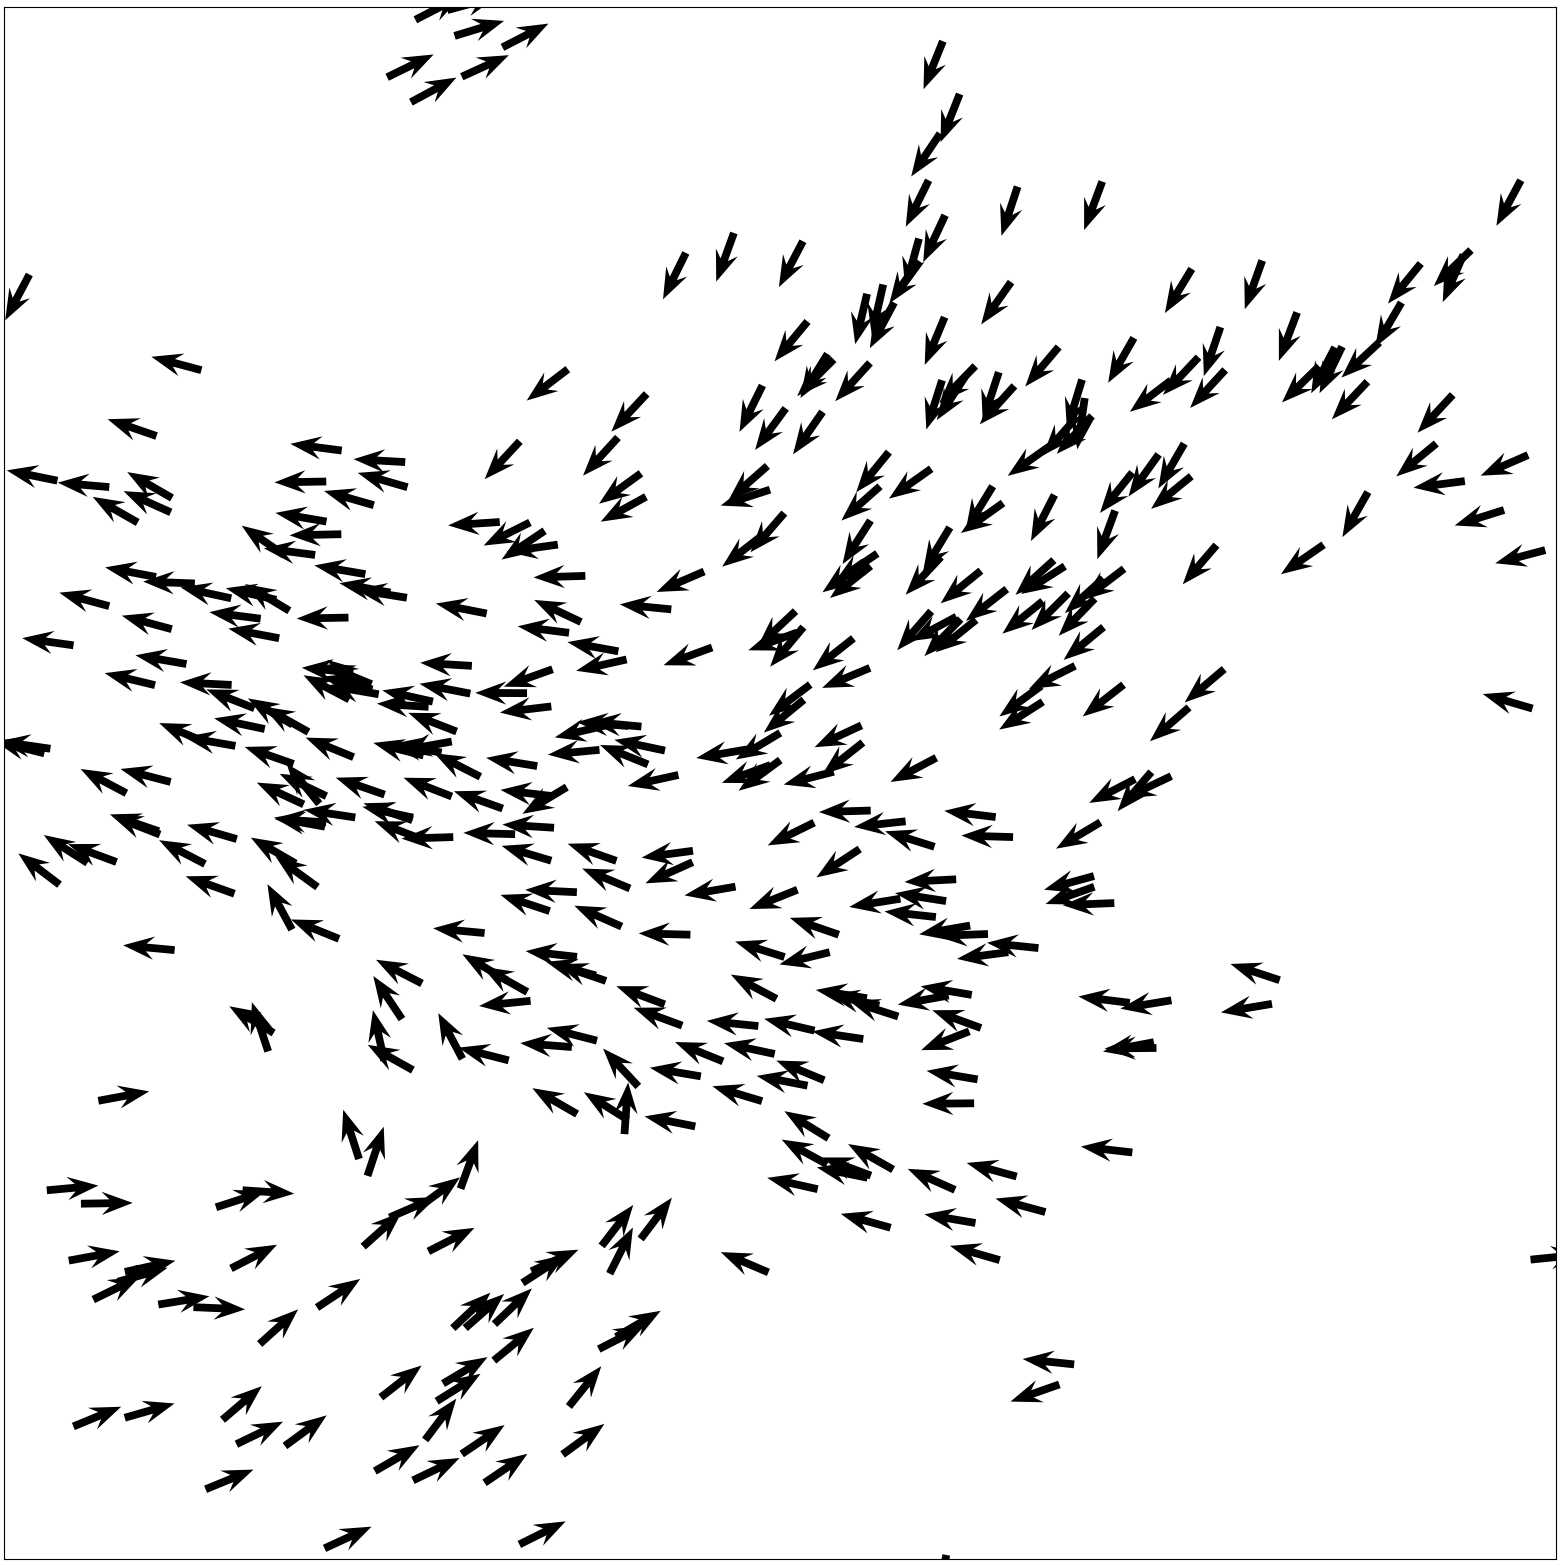
\includegraphics[width=0.3\textwidth]{plots/Snapshot_rk1_n0.4.png}
    \label{fig:Snapshot_rk1_n0.4}
  }
  \subfigure[$k=2$, $\eta=0.6$]{
    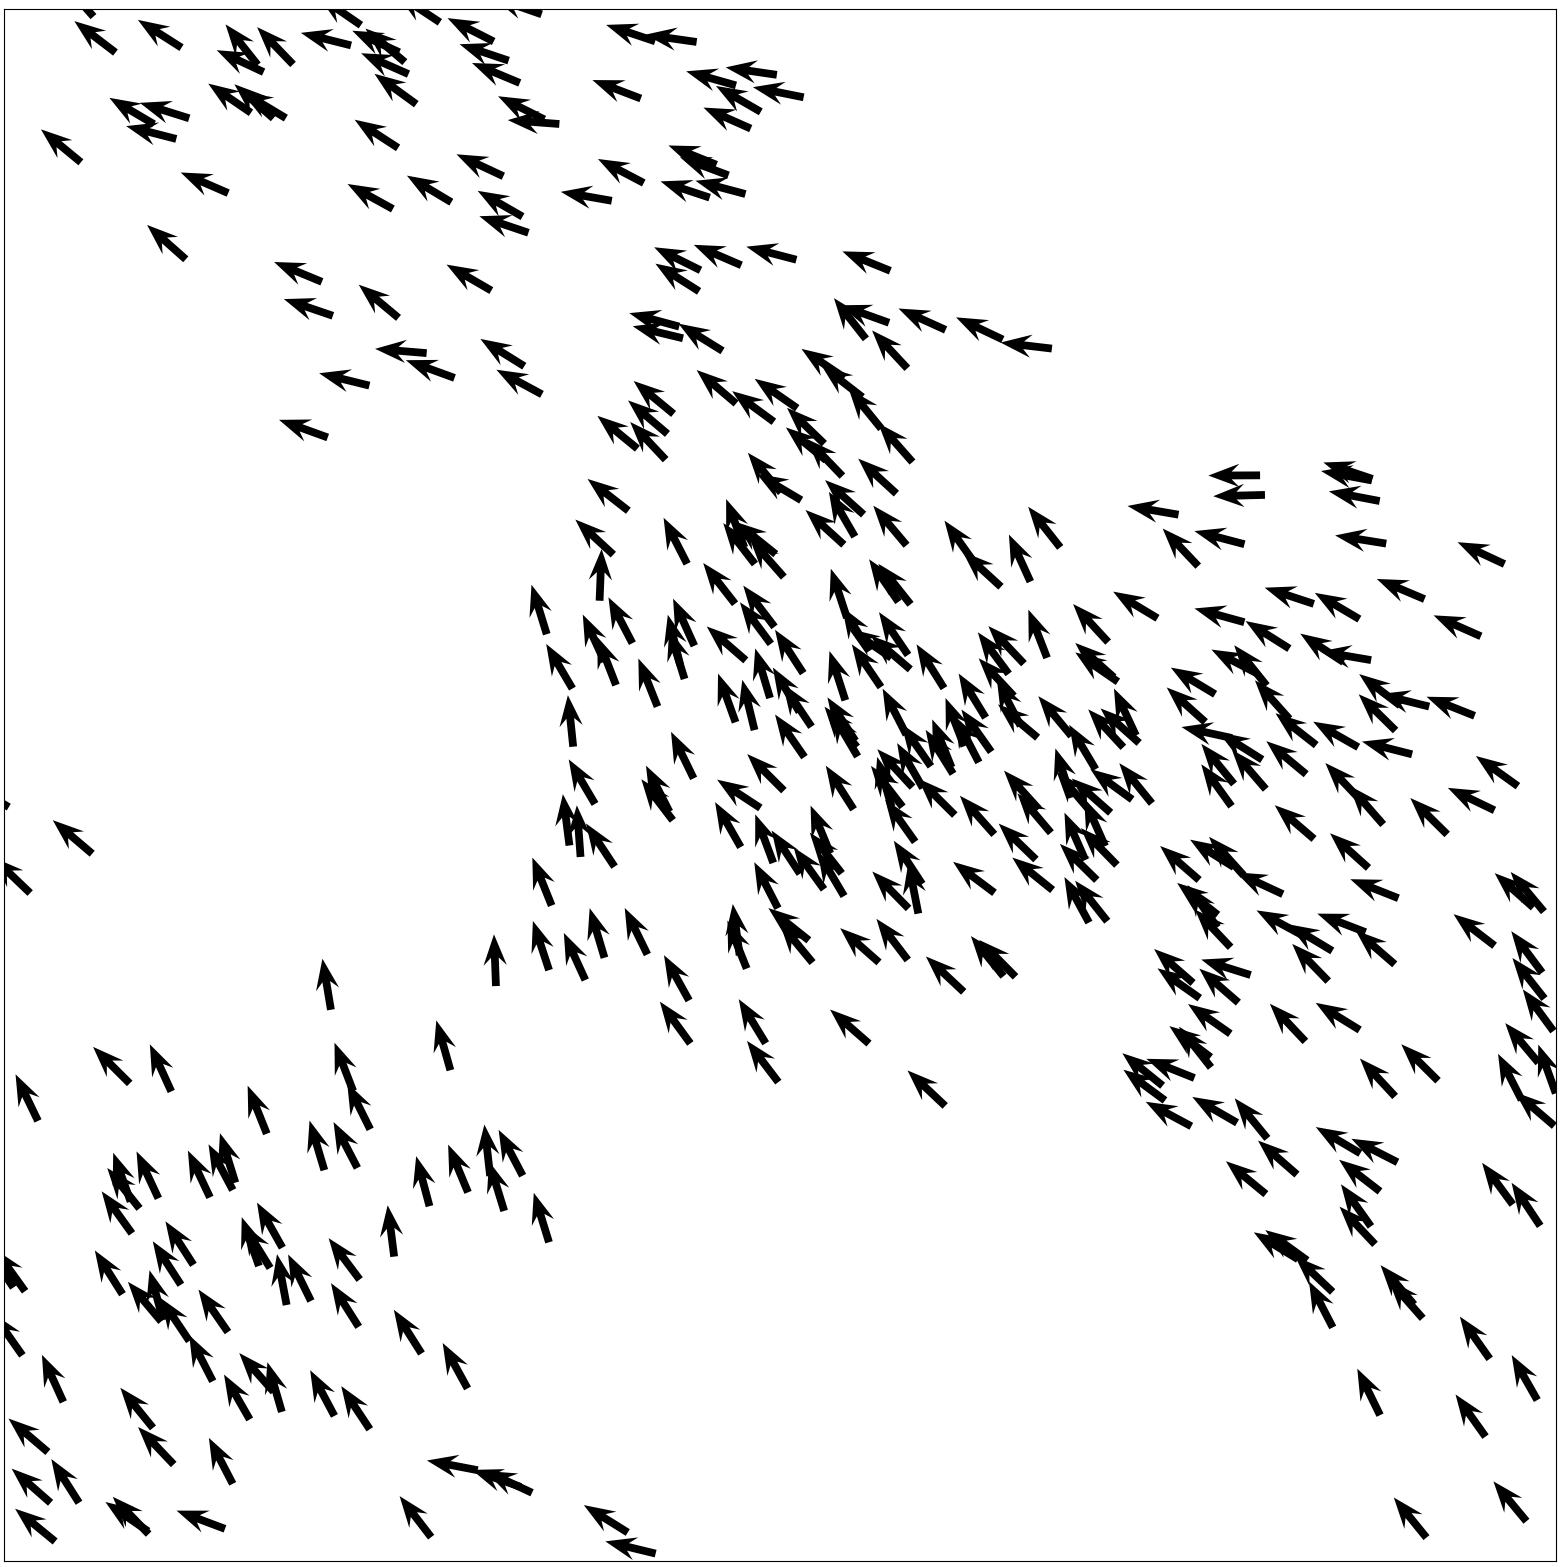
\includegraphics[width=0.3\textwidth]{plots/Snapshot_rk2_n0.6.png}
    \label{fig:Snapshot_rk2_n0.6}
  }
  \subfigure[$k=4$, $\eta=1.0$]{
    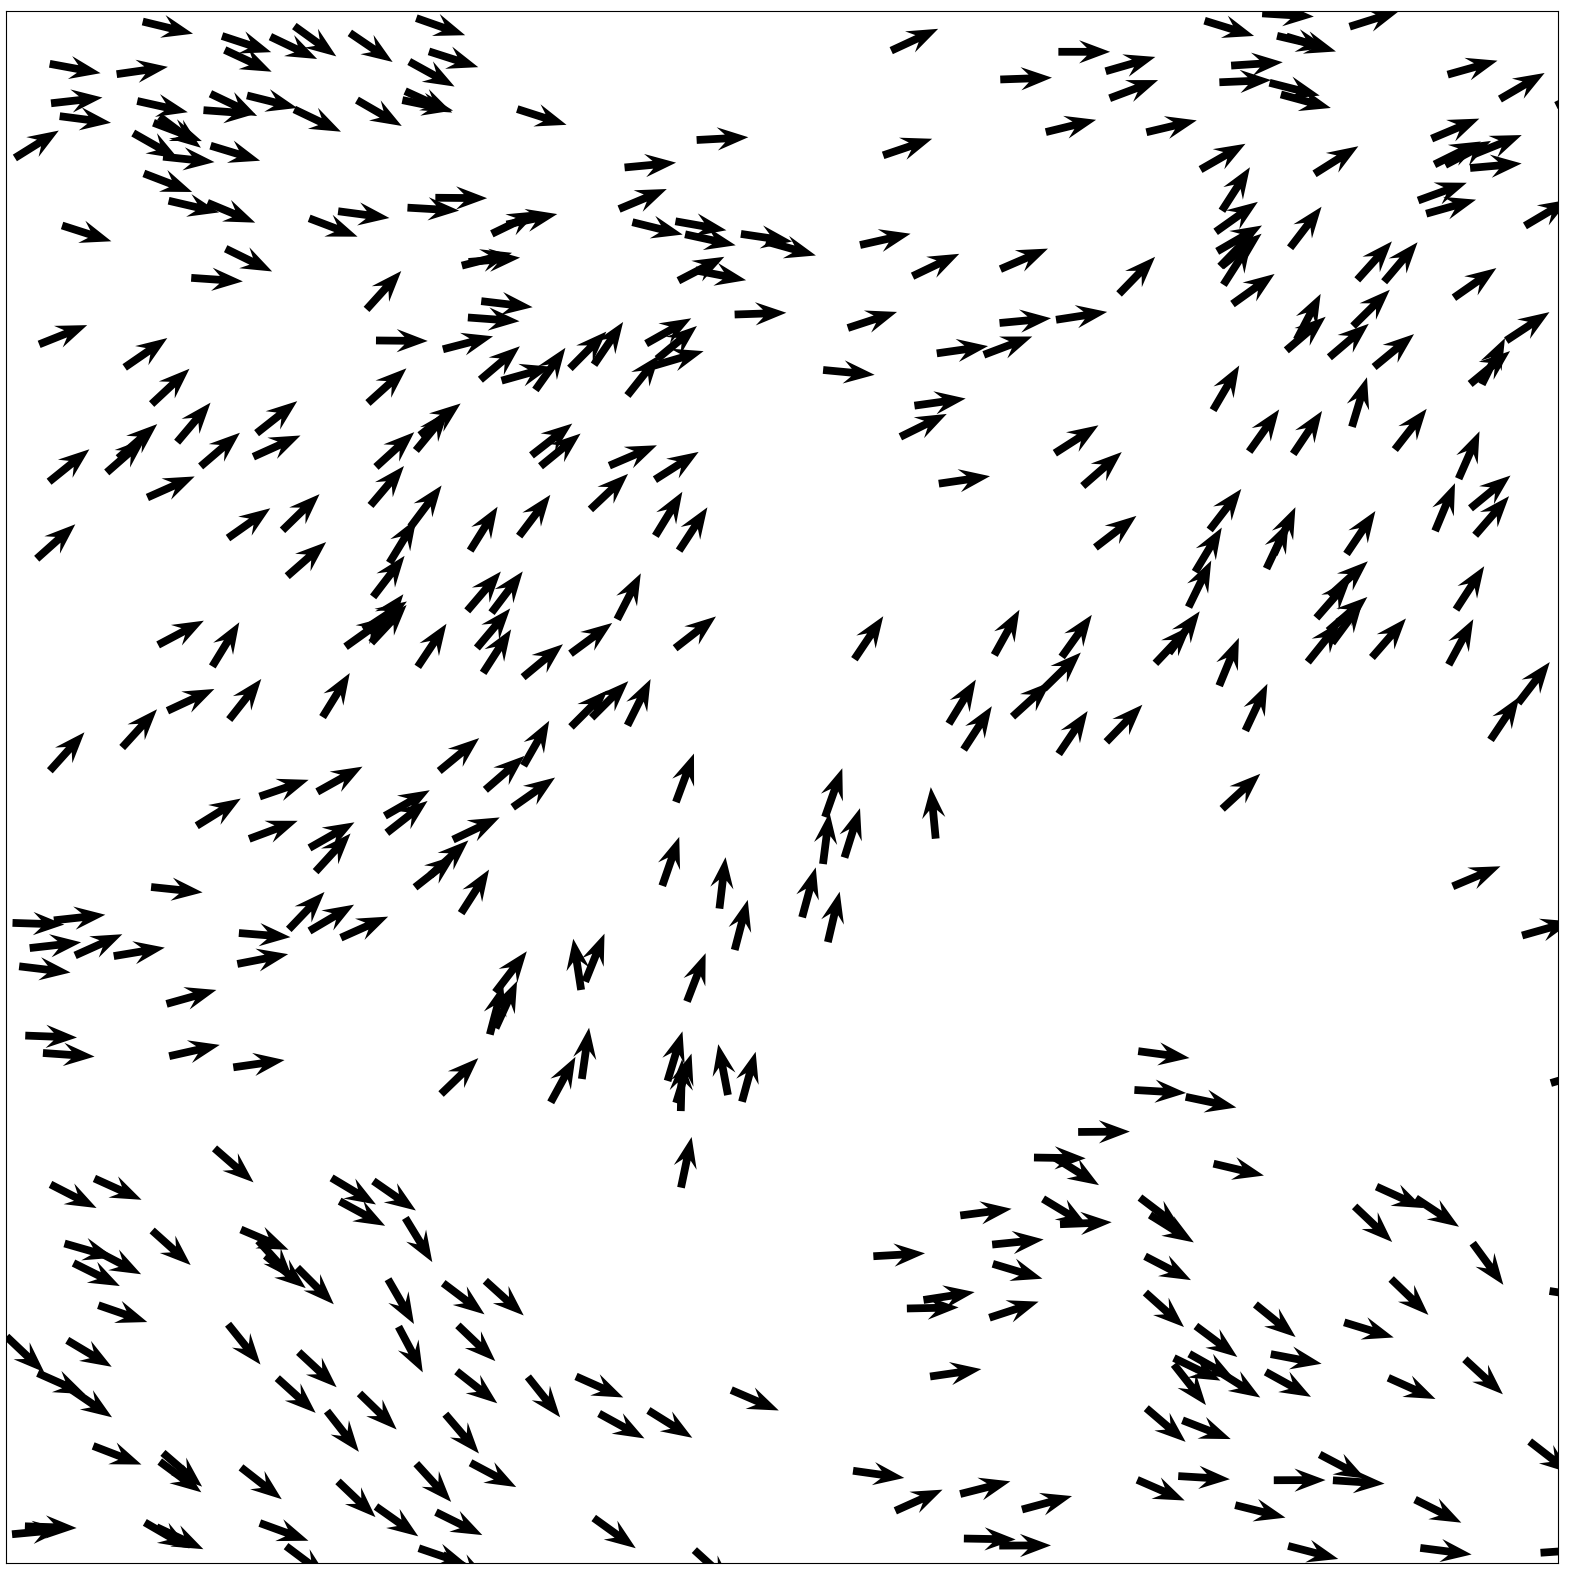
\includegraphics[width=0.3\textwidth]{plots/Snapshot_rk4_n1.0.png}
    \label{fig:Snapshot_rk4_n1.0}
  }
  \caption{Schnappschüsse des metrischen-topologischen Modells mit stochastischer Modifikation. Es ist $N=400$ und $\rho=4$. Alle Schnappschüsse wurden nach nur \textit{sehr} wenigen Simulationsschritten aufgenommen ($\Tilde{t} < \num{20}$).}
  \label{fig:Snapshot_rk_n}
\end{figure}

\subsection{Konvergenz zum Vicsek-Modell}

Das metrisch-topologische Modell konvergiert gegen das Vicsek-Modell für große $k$. Dieser Fall kann leicht konstruiert werden, indem $k > N$ betrachtet wird. In dieser Situation wäre das Modell in der Lage, jede beliebige Teilchenanzahl im Wechselwirkungsradius $r$ gleichzeitig zu berücksichtigen. Dies entspricht aber gerade dem metrischen Modell, wodurch die Konvergenz qualitativ sofort begründet ist. Abbildungen \ref{fig:Convergence_1a_rkFixedRadius_final} und \ref{fig:MSE_vs_k_double} zeigen eine quantitative Untersuchung dieses Konvergenzverhaltens. Für $k=6$ sind praktisch kaum noch Abweichungen erkennbar. Wird der durchschnittliche quadratische Fehler (MSE) gegen die Anzahl der Nachbarn $k$ aufgetragen, ist sofort der exponentielle Abfall der Abweichungen erkennbar. In dem nebenstehenden Plot in Abbildung \ref{fig:MSE_vs_k_double} wird mit einer log-log-Darstellung und einem linearen Fit genau diese exponentielle Beziehung hervorgehoben. Dabei wird beobachtet, dass große Systeme mit vielen Teilchen langsamer konvergieren als kleinere Systeme (bei gleicher Dichte $\rho = 4$).

\begin{figure}[h!]
    \centering
    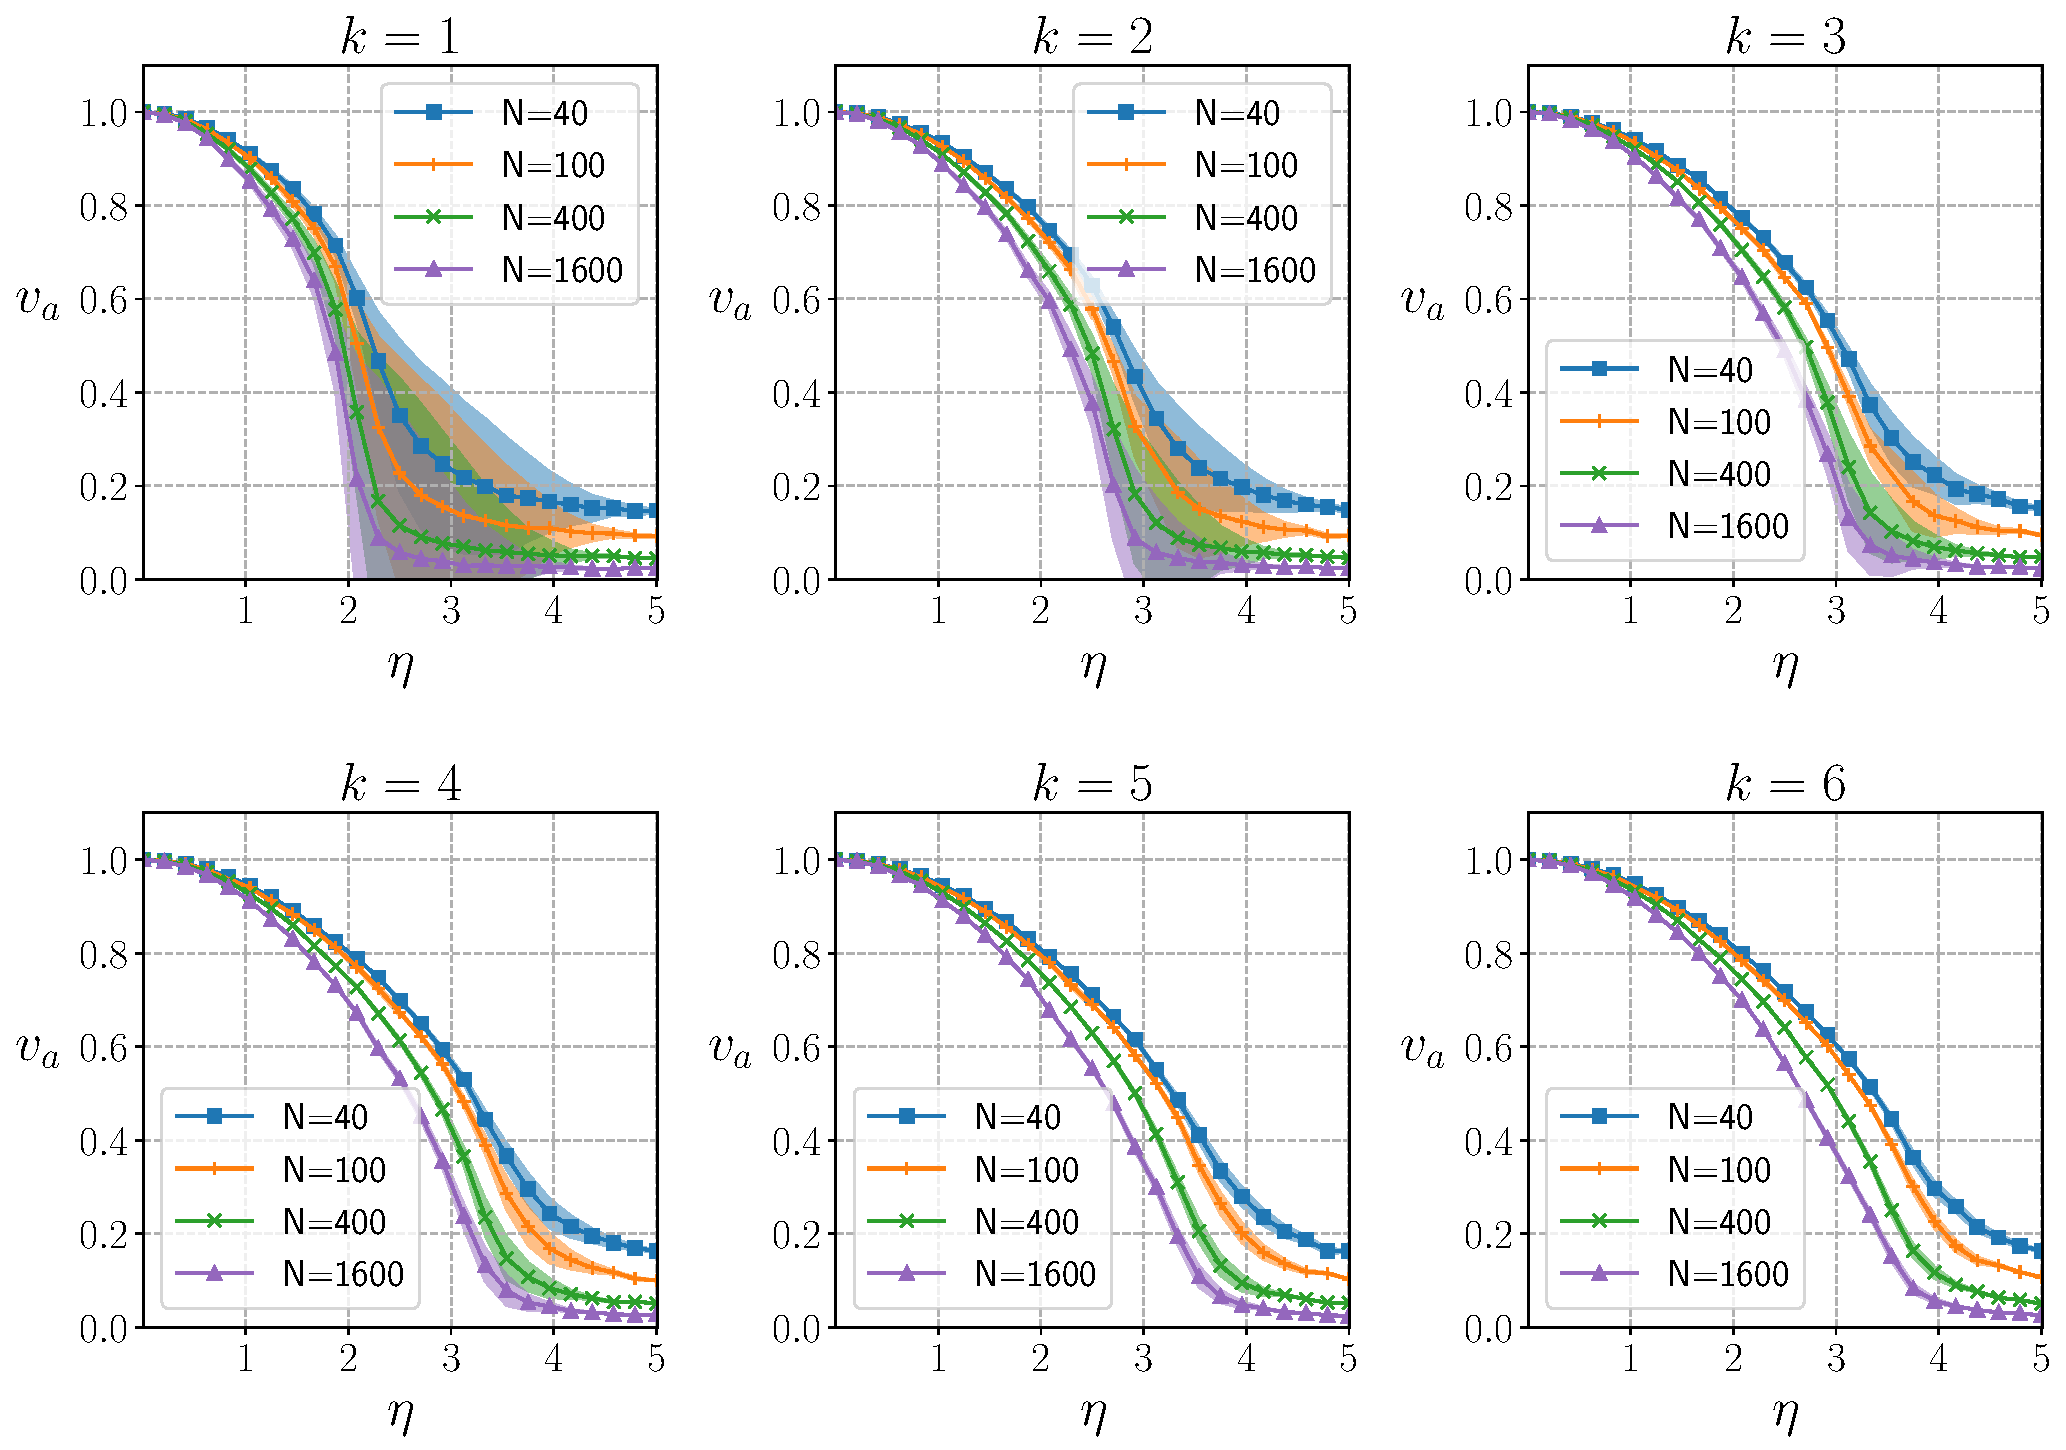
\includegraphics[width=\textwidth]{plots/Convergence_1a_rkFixedRadius_final.pdf}
    \caption{Konvergenz-Analyse und Vergleich des metrisch-topologischen Modells mit dem Vicsek-Modells. Es wird die quadratische Abweichung betrachtet, welche als Schlauch um die Messkurven gelegt ist.}
    \label{fig:Convergence_1a_rkFixedRadius_final}
\end{figure}

\begin{figure}[h!]
    \centering
    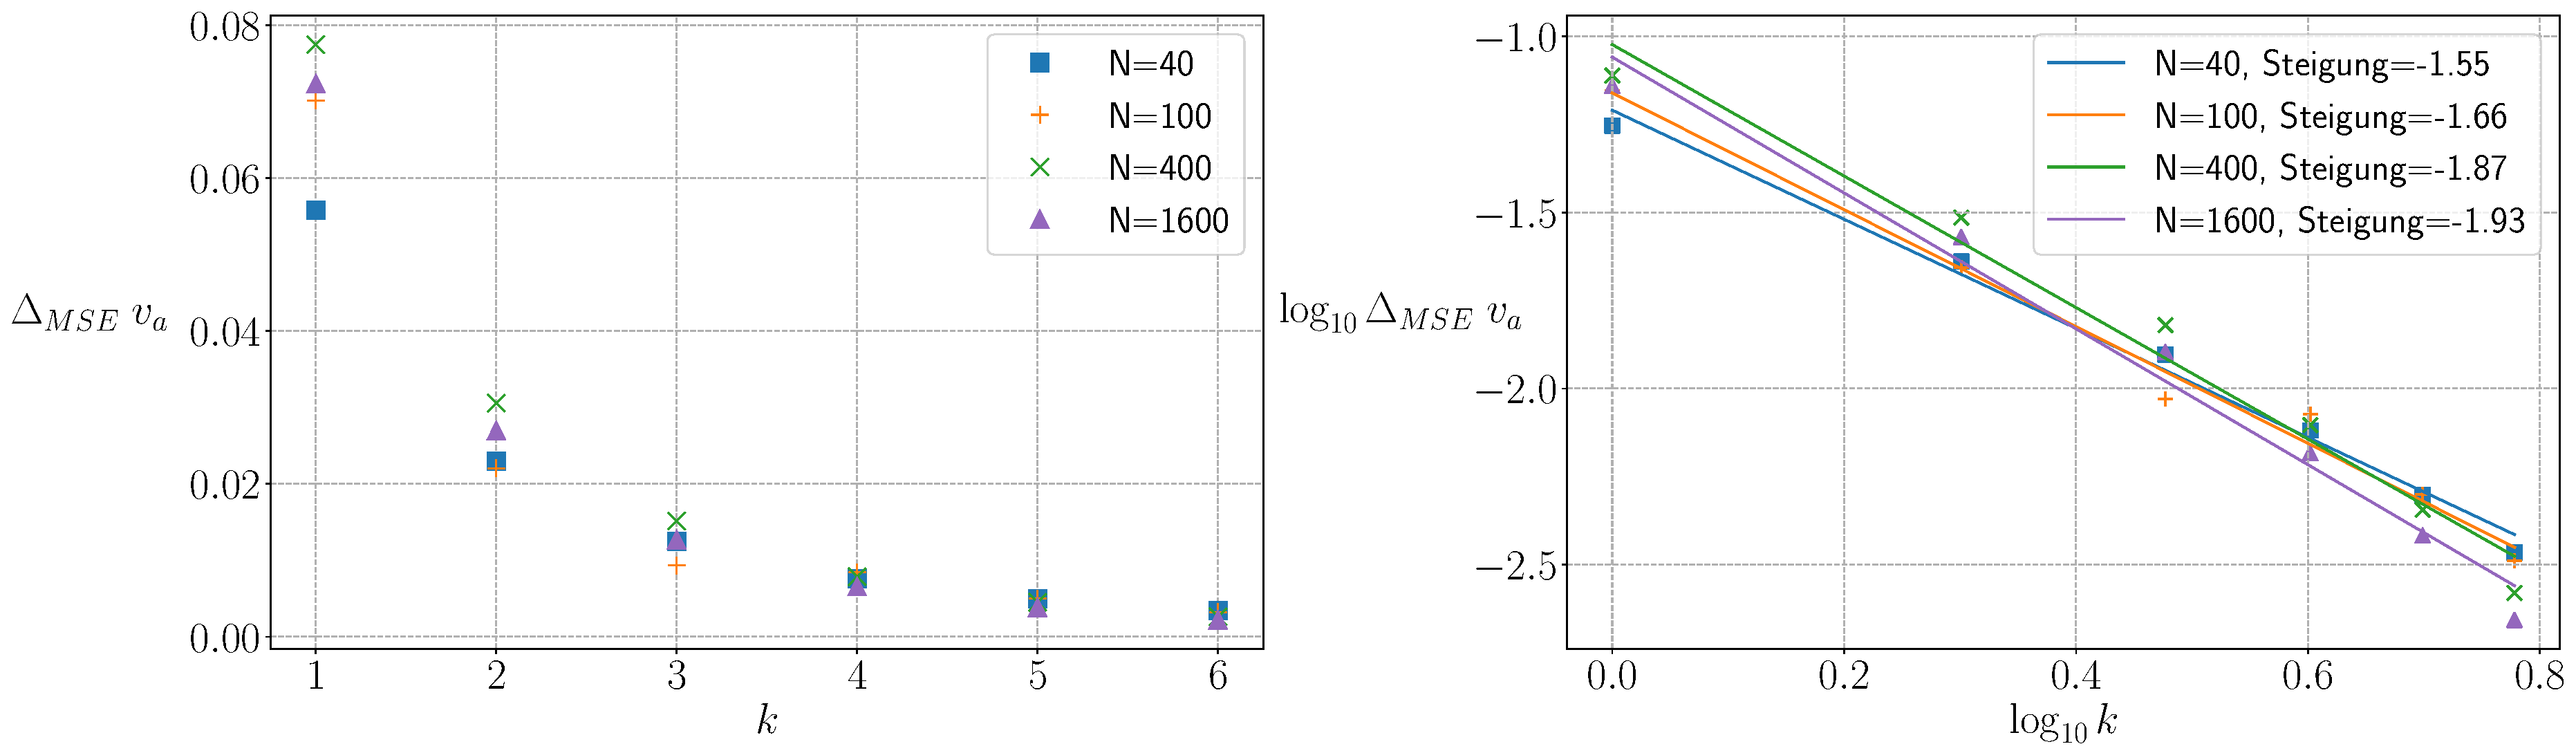
\includegraphics[width=.9\textwidth]{plots/MSE_vs_k_double.pdf}
    \caption{Konvergenz des metrisch-topologischen Modells mit dem Vicsek-Modell. Es wird mit den selbst generierten Daten aus Abbildung \ref{fig:Vicsek_1a} verglichen, nicht mit den Originaldaten. \textbf{Links}: \textit{Mean squared error} (MSE) für jede Gruppierung von $N$ und jedes $k$. \textbf{Rechts}: Eine log-log-Darstellung mit linearem Fit. Die Abweichungen sind stärker, je größer das System bzw. die Teilchenzahlen sind.}
    \label{fig:MSE_vs_k_double}
\end{figure}

\newpage
\subsection{Einführung eines dichtebasierten Ordnungsparameters}
\label{sec:Dichte_Parameter}

Bislang fanden alle Untersuchungen basierend auf nur einem einzigen Ordnungsparameter \eqref{eq:ordnungsparameter_vicsek} statt. Der Vicsek-Ordnungsparameter $v_a$ misst die kollektive Ausrichtung des Schwarms und ist maximal, falls alle Teilchen parallel ausgerichtet sind. Er ist jedoch unabhängig von lokalen Dichtefluktuationen des Systems und macht keine Aussage über die Kompaktheit eines Schwarms. Diese Lücke sollen distanz- bzw. dichtebasierte Ordnungsparameter schließen. Ein möglicher Ansatz ist die distanzbasierte Gewichtung des Skalarproduktes zweier Teilchen:

\begin{equation}
    \highlight{\rho_a=\frac{N(N-1)}{2}\sum_{i<k}^N \Tilde{\vec{v}}_i \Tilde{\vec{v}}_k \frac{1}{\left(\left|\Tilde{\vec{x}}_i-\Tilde{\vec{x}}_k\right|^2+d^2\right)^\frac{\alpha}{2}}=\frac{N(N-1)}{2}\sum_{k=0}^N \sum_{i=k+1}^N \Tilde{\vec{v}}_i \Tilde{\vec{v}}_k d_{ik}(\alpha, d)}
    \label{eq:ordnungsparameter_dichte}
\end{equation}

Es wird dann über alle Teilchen summiert. Um die großen Beiträge sehr naher Teilchen in $d_{ik}$ zu minimieren, kann ein Glättungsfaktor $d$ eingeführt werden. Gleichzeitig kann mit $\alpha$ reguliert werden, wie stark diese Distanzbeiträge in den Ordnungsparameter $\rho_a$ einfließen. In einer weiteren Überlegung kann der Ausdruck in der runden Klammer auch durch $\const{argmax}(d_{ik}^2, d^2)$ ersetzt werden. Wird $d$ dann bspw. auf den Wechselwirkungsradius $r$ gesetzt, bedeutet dies, dass wechselwirkende Teilchen einen maximalen, konstanten Beitrag zum Ordnungsparameter leisten.\\

Abbildung \ref{fig:density_weighted_rkFixedRadius} zeigt die in dieser Arbeit nun schon mehrfach untersuchten Konfigurationen unter Verwendung des stochastischen metrisch-topologischen Modells. Die Werte für $\eta = 0$ sind nicht eingetragen, da diese stark von den Anfangsbedingungen abhängen und der qualitative Verlauf dennoch sehr gut abgelesen werden kann.

Da eine quantitative und qualitative Diskussion von $\rho_a$ in dieser Arbeit eine eher untergeordnete Rolle spielt, befinden sich die Abbildungen dazu im Anhang. Es soll vielmehr gezeigt werden, dass diese Parameter eingeführt werden können und auf ihre Aussagekräftigkeit individuell untersucht werden müssen.

\section{Neuronale Schwarmdynamik mittels Reinforcement Learning}
\label{sec:Neuronale_Schwarmdynamik}
\subsection{Aufbau des Frameworks und des neuronalen Netzwerks}

Für diese Arbeit wurde die bereits erwähnte Bibliothek \texttt{RLlib} verwendet, die viele Werkzeuge für das Aufsetzen eines MARL-Projektes mitliefert \cite{RLlib}. Als Framework für das Maschinelle Lernen bzw. für die neuronalen Netze wurde \texttt{TensorFlow} bzw. \texttt{Keras} verwendet. Wie in der Theorie bereits motiviert wird der PPO Algorithmus verwendet. Das neuronale Netz ist so einfach wie möglich gehalten, da das übergeordnete Ziel dieser Implementierung die Imitation der Vicsek-Regel ist, welche einer einfachen Mittelung entspricht.

In Abbildung \ref{fig:Actor_Netzwerk} ist beispielhaft ein solches Netz gezeigt.

\subsection{Training und Validierung}

Die Implementation ist an dieser Stelle beendet. Das Framework ist aufgesetzt und es wird auch ein Trainingsprozess durchgeführt. Die Multi-Agent Umgebung funktioniert und alle Elemente arbeiten zusammen. Die einzige Ausnahme bildet die Repräsentation des Winkels im Bezug auf das neuronale Netz. Durch diesen Umstand sind die Ergebnisse nicht interpretierbar und das weitere Vorgehen wird im Schluss-Teil diskutiert.

\newpage
\section{Diskussion \& Ausblick}
\label{sec:Diskussion}

Diese Arbeit hat sich intensiv mit den etablierten Modellen der Schwarmdynamik auseinandergesetzt. Es wurde das Vicsek-Modell und seine topologische Modifikation implementiert und validiert. Die Suche nach einem brauchbaren Modell für das Maschinelle Lernen führte schließlich auf das neuartige metrisch-topologische Modell. All diese Modelle wurden rigoros untersucht, um die jeweiligen Stärken und Schwächen zu untersuchen.

\subsubsection*{Multi-Agent Reinforcement Learning}

Der Kern dieser Arbeit beschäftigt sich mit der Frage, ob eine Schwarmdynamik durch neuronale Netze gelernt bzw. approximiert werden kann. Da es sich bei der Schwarmdynamik um Vielteilchensysteme handelt, muss ein Multi-Agent Framework verwendet werden. Diese Algorithmen sowie Frameworks sind so neu, dass sie aktuell einer sehr starken Entwicklung unterliegen. Daher war es besonders schwierig, sich nicht nur in das komplexe Thema des Reinforcement Learnings einzuarbeiten, sondern auch die notwendige Software aufzusetzen und zu testen. Es floss sehr viel Arbeit in die Konzeption und Erprobung dieser Umsetzung. Große Teile der Arbeit sind leider nicht visualisierbar.\\

Dennoch steht zum Schluss dieser Arbeit ein zentrales Ergebnis: Die mühsam erprobte \texttt{C++} Simulation ist nun vollständig eingebettet in ein funktionierendes, trainierendes Framework von \texttt{RLlib}. Einmal aufgesetzt ist das Training vergleichsweise einfach, sodass nun ein neuer Abschnitt der Arbeit beginnen würde. Da die Änderung des Ordnungsparameters als Belohnungs-Funktion verwendet werden kann, können nun beliebig komplexe oder einfache Systeme untersucht werden.\\

Interessant wäre die Frage, ob ein einzelnes \textit{single-layer} Perzeptron, also das einfachste Modell eines neuronalen Netzes, ausreicht, um die Vicsek-Mittelungsregel zu lernen. Die Vermutung ist: \textbf{Ja}. Diese Hypothese galt es zu testen, was wegen der zeitlichen Beschränkung dieser Arbeit leider knapp verpasst wurde.

Die Möglichkeiten, die nun offenstehen, sind zahlreich. Abbildung \ref{fig:SwarmModelInfoChart} zeigt eine Übersicht, die die Komplexität und Reichweite dieser Arbeit verdeutlichen soll. Es gibt zahlreiche interessante Variationen der Modelle und diese können beliebig um komplexere Elemente ergänzt werden.\\

Die modernen Algorithmen des Maschinellen Lernens haben sich vor allem bei komplizierten Aufgabenstellungen zunehmend bewiesen. Die Frage ist also vermutlich nicht \textit{ob} diese Methoden komplexe Aufgaben der Schwarmdynamik lösen können, sondern \textit{wie}.

\subsubsection*{Vicsek-Modell: Abweichungen zur Originalarbeit}

Der Vergleich in Abbildung \ref{fig:Vicsek_1a} zeigt zunächst einen qualitativ gleichwertigen Verlauf der Messkurven. Ein genauerer Blick auf die höheren Rauschwerte (ab etwa $\eta \geq 3$) deckt jedoch Unstimmigkeiten mit den originalen Messdaten auf. Die Gründe für diese Abweichungen sind unbekannt und können in dieser Arbeit nicht vollständig beantwortet werden. Dennoch werden mehrere potenzielle Fehlerquellen gründlich geprüft und ausgeschlossen.\\

\begin{itemize}
    \item \textbf{Fehlerquellen im Code:} Ein Großteil der Entwicklungszeit wurde für die Validierung des Modells und das Ausschließen möglicher Fehler im Code aufgewendet: Die Bestimmung der nächsten Nachbarn, die Modell-Regeln, Periodische Randbedingungen, Distanzmessungen, propagierende Rundungsfehler und eine sorgfältige Auswahl der Zufallsgeneratoren sind alles Aspekte, die mehrfach untersucht und zum großen Teil auch visuell geprüft wurden.
    \item \textbf{Statistische Ungenauigkeiten:} Wie bereits erwähnt, werden keine fortgeschrittenen statistischen Methoden oder Tests verwendet. Die Stabilität der Messwerte wurde untersucht, indem unterschiedliche Simulationszeiten miteinander verglichen wurden. Zudem wurden verschiedene Anfangsbedingungen getestet; einschließlich solcher, die in einem vollständig geordneten Zustand beginnen. Die Ergebnisse konvergieren für eine gegebene Parameterkonfiguration unabhängig von den Anfangsbedingungen immer gegen den gleichen Wert. Der glatte Verlauf der Messwerte legt nahe, dass es sich um Gleichgewichtszustände handelt.
    Der Verdacht kann auch auf den laufenden Durchschnitt fallen, der durch die frühe Mitnahme von Messwerten sicherlich leicht gebiased ist. Dieser Bias würde sich aber Richtung $v_a \rightarrow 0$ (da das System zu Beginn ungeordnet ist) und damit entgegen der beobachteten Abweichung bewegen. Damit wird eine statistisch motivierte Abweichung unwahrscheinlich, obwohl dies durch den Vergleich mehrerer Messungen und der Anwendung zuverlässigerer statistischer Methoden überprüft werden müsste.
\end{itemize}

Auch Abbildung \ref{fig:Vicsek_1b} weist Abweichungen auf, die jedoch ebenfalls schwierig zu untersuchen sind, da aus der originalen Arbeit nicht alle Implementierungs- und Auswertungsdetails bekannt sind. Es ist nicht bekannt, bei welchem Rauschen $\eta$ diese Messungen durchgeführt werden. Die Abweichung kann eventuell so verstanden werden, dass sich die Kurve, die in dem originalen Plot zu sehen ist, durch ihre Abhängigkeit von $\eta$ nach links verschiebt. Dann wären die Messergebnisse wieder plausibel. Dies könnte geprüft werden, indem die Messungen bei anderen Rauschwerten durchgeführt werden.

\subsubsection*{Ausblick}

Die Ergebnisse dieser Arbeit bieten eine große Bandbreite an möglichen Weiterentwicklungen. Unabhängig von dem Maschinellen Lernen können die Ordnungsparameter weiter untersucht werden. Diese Parameter entspringen häufig der Intuition oder Erfahrung und können wertvolle Informationen des Systems beinhalten. Verschiedene Ordnungsparameter können verschiedene Aspekte des Systems beleuchten. Können diese Parameter analytisch abgeleitet werden, ergibt sich eventuell sogar eine Regel, die neuartige Muster zeigen kann. An dieser Stelle greift wieder der Reinforcement Learning Ansatz. Durch diese Methode können mehrere Ordnungsparameter miteinander kombiniert werden und das System lernt eigenständig die für die Optimierung dieser Parameter notwendigen Regeln.\\

Diese Arbeit verdeutlicht, dass die Schwarmdynamik weit mehr ist als nur ein theoretisches Konstrukt, sondern ein Schlüssel zur Enthüllung der Geheimnisse kollektiver Intelligenz und adaptiver Systeme. Sie markiert einen Meilenstein in der Annäherung zwischen klassischer Physik und modernen maschinenlernbasierten Methoden und lädt zur weiteren, tiefgreifenden Forschung in diesem faszinierenden interdisziplinären Feld ein.


\appendix
\newpage
\section{Plots}

\begin{figure}[h!]
    \centering
    
\includegraphics[width=.9\textwidth]{plots/density_weighted_rkFixedRadius.pdf}
    \caption{Untersuchung des dichtebasierten Ordnungsparameters $\rho_a$ für das stochastische metrisch-topologische Modell. Im Gegensatz zu dem Ordnungsparameter $v_a$ equilibriert das System nie gegen $\rho_a = 1$. Die Systemdichte ist $\rho = 4$ und die Parameter zur Regulierung sind $\alpha = 1$ und $d = r$.}
    \label{fig:density_weighted_rkFixedRadius}
\end{figure}

\newpage
\section{Illustrationen}

\begin{figure}[h!]
    \centering
    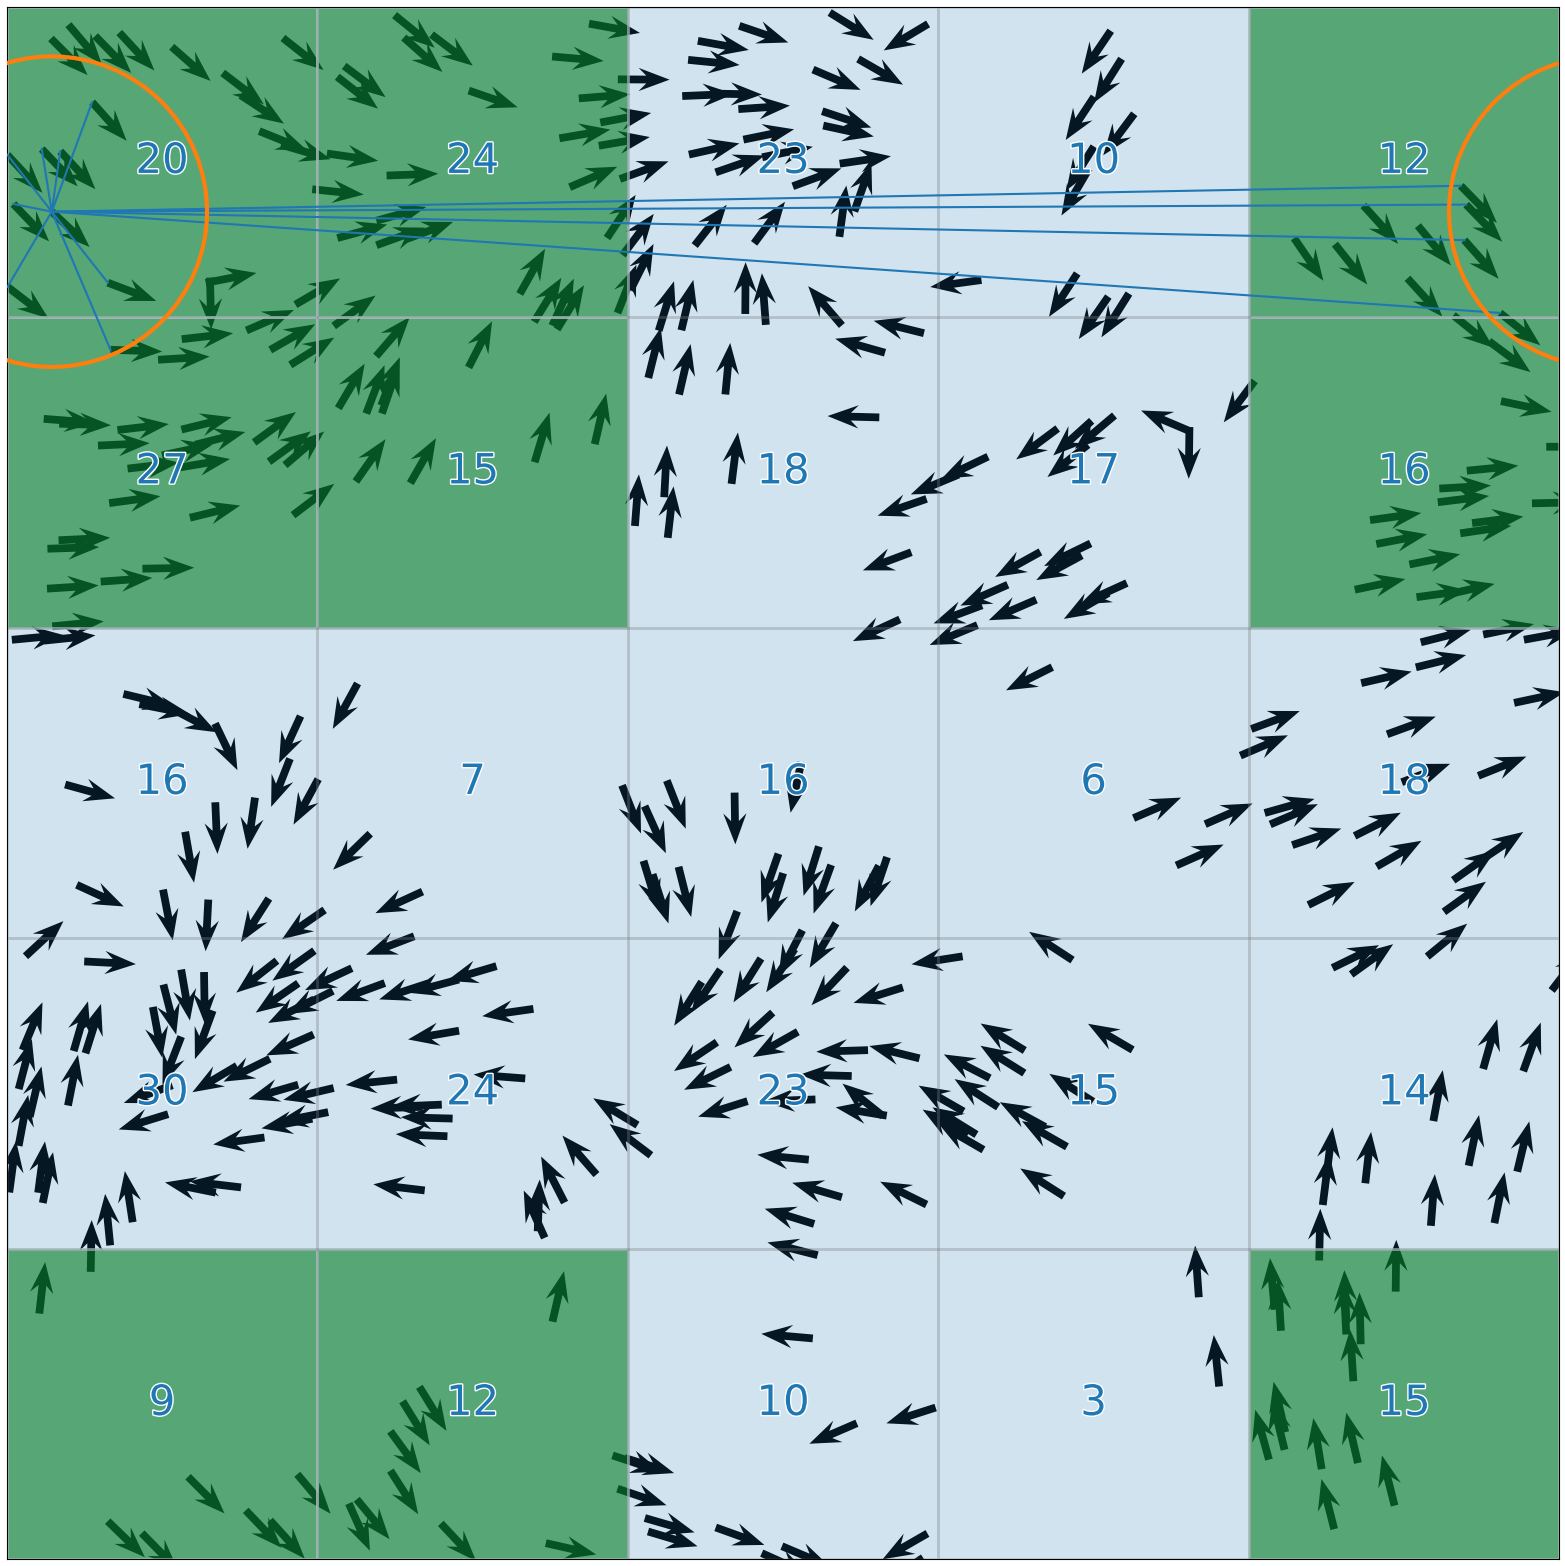
\includegraphics[width=\textwidth]{illustrations/VisuellesDebugging.png}
    \caption{Visuelles Debugging durch die Darstellung der wichtigsten Komponenten der Simulation. \textbf{Konfiguration}: $N = 400$, $\rho = 4$, $\eta = 0.1$, metrisches Modell, Vicsek-Regel. Die Teilchenposition entspricht der Basis eines Pfeils (unteres Ende).\\
    Simulation mit einem üblichen Randfall. In dieser Visualisierung sind neben den Teilchen selbst auch die Simulationszellen und ihre Teilchenanzahl abgebildet. Es ist exemplarisch für ein Teilchen der Wechselwirkungsradius $r$ eingezeichnet und es wird mit Verbindungslinien kenntlich gemacht, welche Nachbarn bestimmt wurden. Die \textcolor{DTUGreen}{grünen Quadrate} geben jene Zellen an, über die zur Ermittlung der Nachbarn iteriert wurde. Es ist erkennbar, dass der Randfall korrekt abgehandelt wird und die Nachbarn auch über den Simulationsbereich hinaus bestimmt werden. Weitere Details sind ausgeblendet, um die Abbildung nicht zu überladen. Aus den zusätzlichen Einstellungen wäre bspw. aber auch erkennbar, dass die Distanzmessungen den Randfall ebenfalls korrekt behandeln und die Distanzen nicht einfach der Länge der Verbindungslinien entsprechen.}
    \label{fig:VisuellesDebugging}
\end{figure}

\begin{figure}[h!]
  \centering
  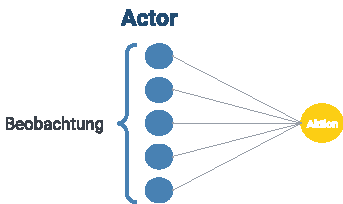
\includegraphics[width=0.5\textwidth]{illustrations/Actor_Netzwerk.pdf}
  \caption{Ein Perzeptron mit nur einer Schicht dient als Grundlage für diese Arbeit.}
  \label{fig:Actor_Netzwerk}
\end{figure}

\begin{figure}[h!]
    \centering
    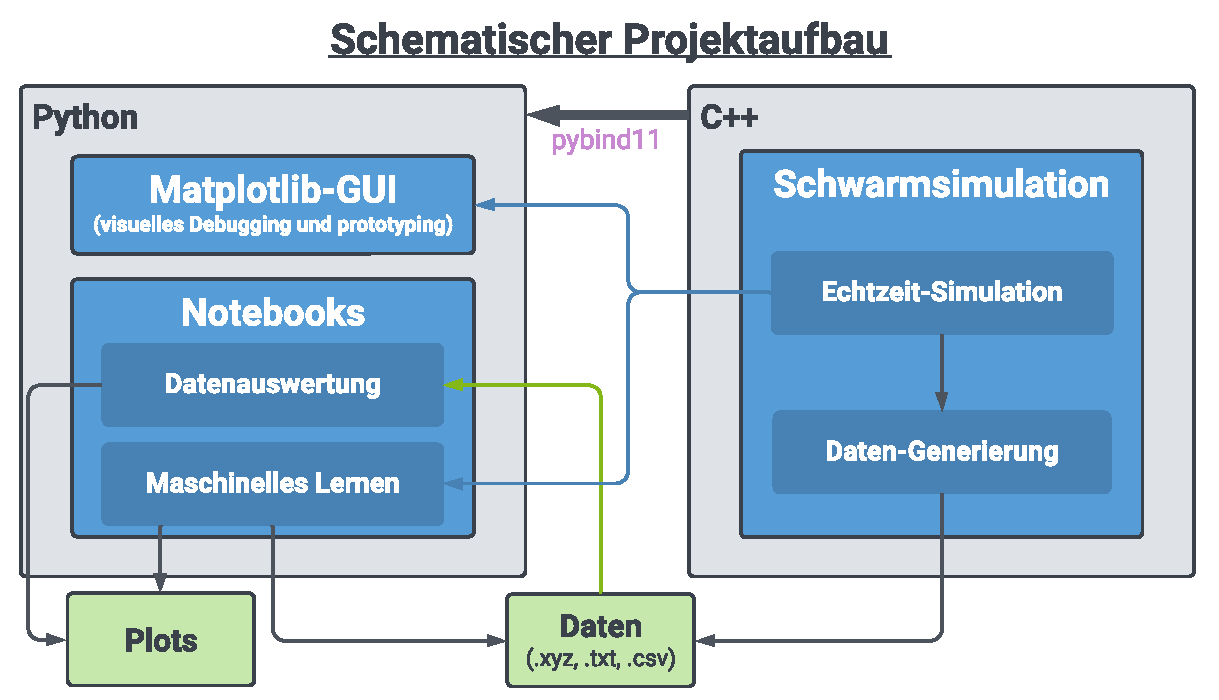
\includegraphics[width=.9\textwidth]{illustrations/SchematischerProjektaufbau.pdf}
    \caption{Schematischer Projektaufbau; Zusammenspiel zwischen \texttt{C++} und \texttt{Python}.}
    \label{fig:SchematischerProjektaufbau}
\end{figure}

\begin{figure}[h]
    \centering
    
\includegraphics[width=\textwidth]{illustrations/SwarmModelInfoChart.pdf}
    \caption{Übersicht der verschiedenen Aspekte des Projekts. Diese Zusammenstellung dient als Orientierungshilfe und skizziert die verschiedenen Vertiefungsmöglichkeiten. Die in dieser Arbeit untersuchten bzw. angewandten Aspekte sind mit einem \textcolor{DTUGreen}{grünen Haken} 
\includegraphics[height=1em]{illustrations/Haken.png} markiert.}
    \label{fig:SwarmModelInfoChart}
\end{figure}

%%%%%%%%%%%%%%%%%%%%%%%%%%%%%%%%%%%%%%%%%%%%%%%%%%%%%%%%%%%%
% Add these commands below if it's not a problem for you 
\thispagestyle{fancyplain}
\fancyhead{}
\renewcommand{\headrulewidth}{0pt}
%%%%%%%%%%%%%%%%%%%%%%%%%%%%%%%%%%%%%%%%%%%%%%%%%%%%%%%%%%%%
\clearpage
\pagestyle{fancy} % clears the middle part of the headers from here on (no year to specify)
\markboth{\textsc{Literatur}}{\textsc{Literatur}} % ensures headers are working as intended during reference chapter
\printbibliography[heading=bibintoc, title=Literatur]

\markboth{\textsc{Bildverzeichnis}}{\textsc{Bildverzeichnis}}
\printbibliography[heading=bibintoc, title=Bildverzeichnis, keyword=bildverzeichnis]
%\section*{Bildverzeichnis}
\newpage
\section*{Danksagung}

Ich möchte an dieser Stelle die Gelegenheit nutzen, Dank auszusprechen. In erster Linie danke ich Herrn Kierfeld für die Betreuung bei diese Arbeit. Ich danke für die transparente Kommunikation einer realistischen Erwartungshaltung und für das Ernstnehmen dieses Abenteuers. Ich möchte auch meinen Dank an Felix aussprechen, der mir wertvolle Ideen und Feedback hat zukommen lassen. Ich empfand die Gesprächsstunden mit euch stets als entspannt, einladend und geistreich.\\

Ich danke vor allem auch Lara, die so viel Rücksicht und Herz gezeigt hat, dass vieles erst durch sie möglich wurde.\\

An dieser Stelle möchte ich auch allen danken, die über die Arbeit drübergeschaut haben; vor allem auch Christian, der sich selbst etwas Zeit an seinem Geburtstag genommen hat, um mich zu unterstützen.\\

Letztlich möchte ich auch allen danken, die bis hier hin an mich geglaubt und mich unterstützt haben.
\newpage
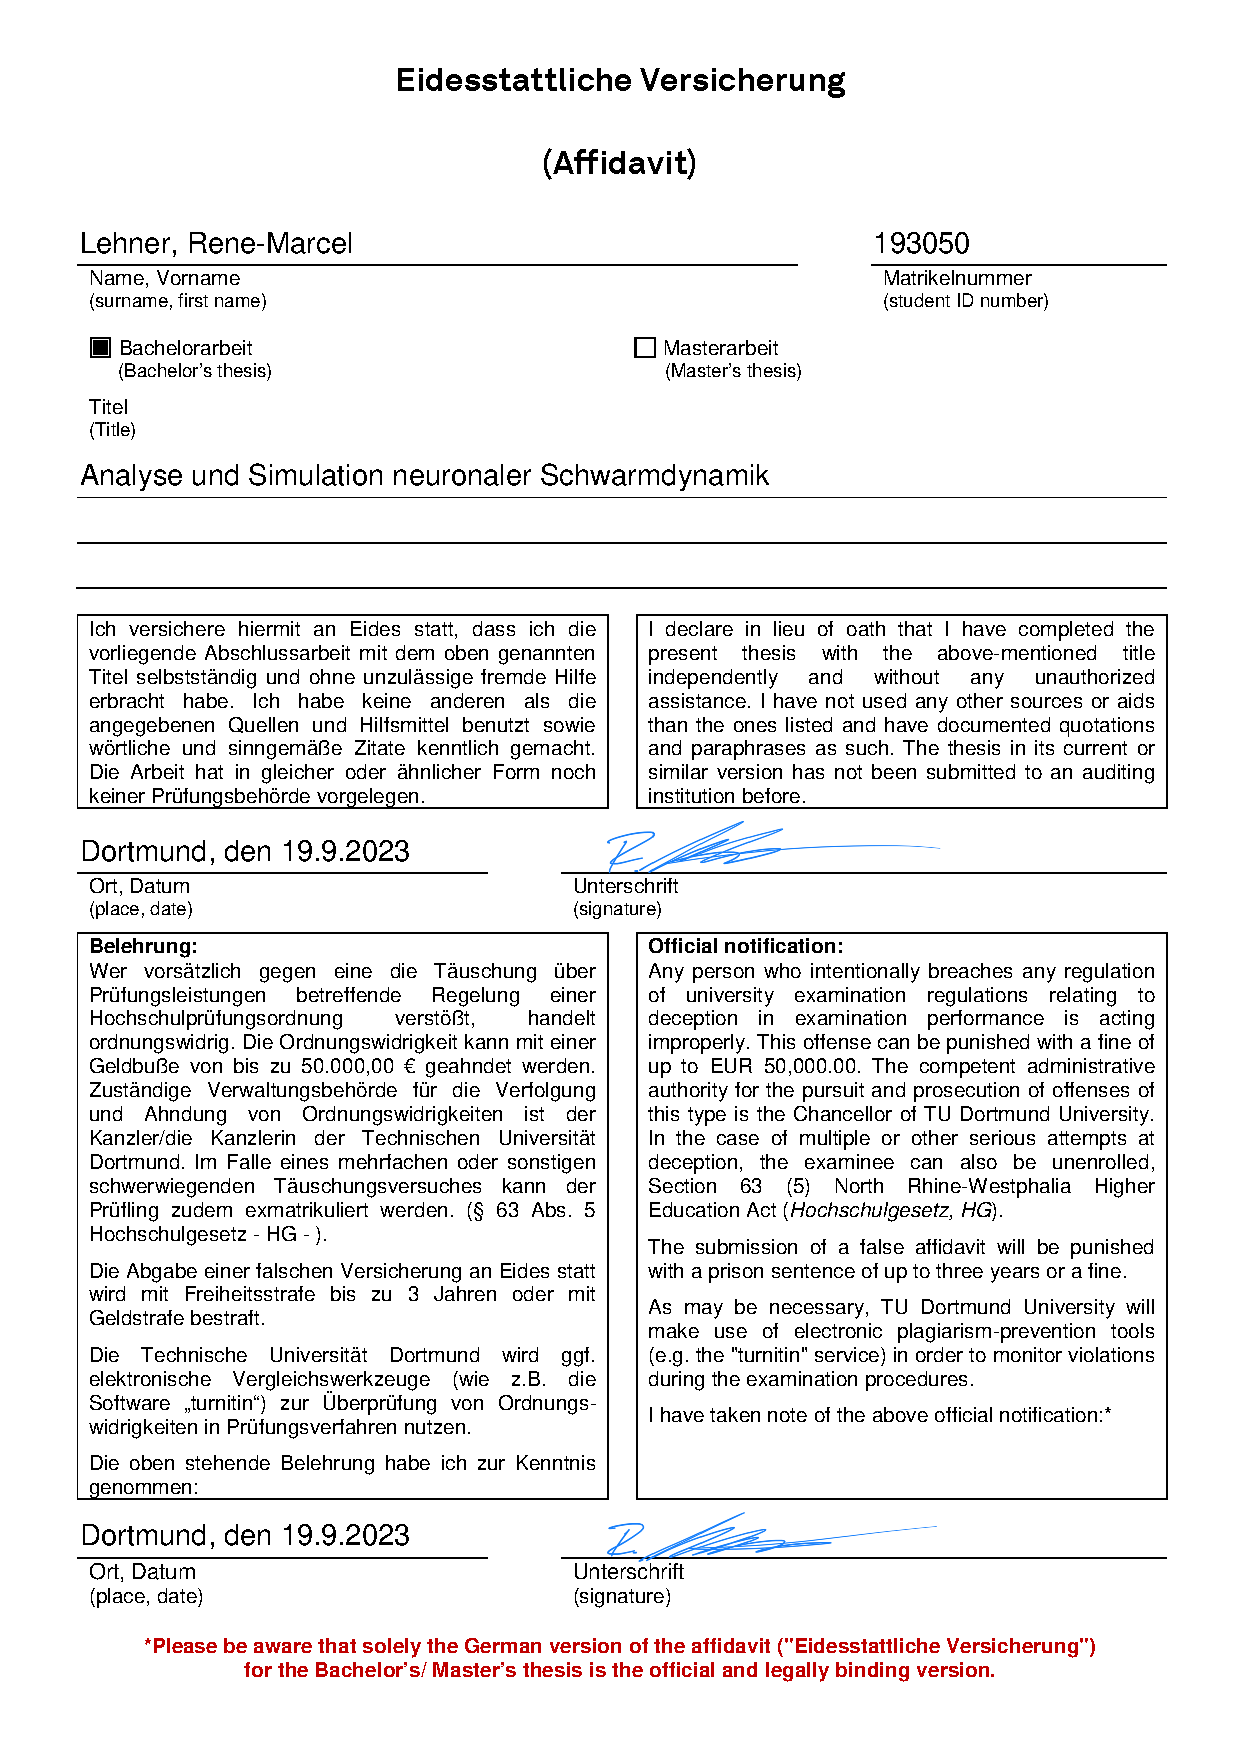
\includepdf[pages=-]{Eidesstattliche_Versicherung_.pdf}
\end{document}